%========================================================================
%  Master Thesis / Working Paper -- Main file
%  xLSTM & Conformal Prediction for Sovereign Credit Spread Forecasting
%  TU Wien, MSc Financial & Insurance Mathematics
%
%  Overleaf import:  zip this folder and "Upload Project", OR sync via GitHub.
%  Compile with pdfLaTeX (Menu -> Recompile). Uses biblatex+biber.
%========================================================================
\documentclass[11pt,a4paper]{article}

%------------------------------------------------------------------ packages
\usepackage[utf8]{inputenc}
\usepackage[T1]{fontenc}
\usepackage[english]{babel}
\usepackage{amsmath,amssymb,amsthm}
\usepackage{bm}                     % bold math symbols
\usepackage{booktabs}               % professional tables
\usepackage{graphicx}
\usepackage{subcaption}
\usepackage{siunitx}                % aligned numbers in tables
\usepackage{algorithm}
\usepackage{algpseudocode}
\usepackage[hidelinks]{hyperref}
\usepackage{cleveref}
\usepackage{geometry}
\usepackage{csquotes}
\geometry{margin=2.5cm}

%------------------------------------------------------------------ bibliography
\usepackage[backend=biber,style=authoryear,natbib=true,maxbibnames=99]{biblatex}
\addbibresource{references.bib}

%------------------------------------------------------------------ shortcuts
\newcommand{\Real}{\mathbb{R}}
\newcommand{\Prob}{\mathbb{P}}
\newcommand{\Exp}{\mathbb{E}}
\newcommand{\Ind}{\mathbf{1}}       % indicator function
\newcommand{\spread}{s}             % level spread
\newcommand{\dspread}{\Delta s}     % delta spread (the modelling target)
\newcommand{\alphamis}{\alpha}      % miscoverage level
\DeclareMathOperator*{\Quantile}{Quantile}

\theoremstyle{definition}
\newtheorem{definition}{Definition}
\newtheorem{assumption}{Assumption}

%========================================================================
\begin{document}

\title{Conformal Prediction Intervals for Sovereign Credit Spread
Forecasting: An xLSTM and Foundation-Model Study}
\author{Felix Neuwirth\\ \small TU Wien -- MSc Financial \& Insurance Mathematics}
\date{\today}
\maketitle

\begin{abstract}
% TODO: 150--250 words. State (i) problem: distribution-free interval
% forecasts for euro-area sovereign spreads; (ii) methods: benchmark suite
% from random walk to xLSTM plus a zero-shot foundation model, wrapped in a
% CQR-based conformal layer with adaptive recalibration; (iii) headline
% finding + the contamination caveat for the zero-shot model.
\end{abstract}

% Sections 1-2 (Introduction, Related Work) live outside this skeleton for now.
% \input{sections/introduction}
% \input{sections/related_work}

%========================================================================
\section{Data and Target Construction}
\label{sec:data}

% Flughöhe: Eine kompetente Person soll dies OHNE deinen Code reimplementieren
% können. Beschreibe WAS und WARUM, nicht Funktionssignaturen.

\subsection{Country universe and sample period}
\label{sec:data:universe}

We study monthly sovereign credit spreads for ten euro-area issuers
(Austria, Belgium, Spain, Finland, France, Greece, Ireland, Italy, the
Netherlands, and Portugal). The spread is the difference between the ECB-10y yield of a country and Germany (ECB dataset IRS, series key M.{cc}.L.L40.CI.0000.EUR.N.Z). The sample runs from 2003-04
to 2026-04: the start is the first month, and the end the last month, in which
all required data points are simultaneously available.

Greece is an exception. In 2015-07 there was no market data because of the
capital controls during the Greek crisis. This missing window is carried forward and doesn't lie in the test set. A second limitation of including Greece is the 2012 private-sector
involvement, which produced a structural break in the spread data.

\subsection{Target variable: delta-spreads}
\label{sec:data:target}

Let $\spread_{i,t}$ denote the level credit spread of country $i$ at time
$t$. All models are trained on the \emph{first difference}
\begin{equation}
  \dspread_{i,t} \;=\; \spread_{i,t} - \spread_{i,t-1},
  \label{eq:delta-target}
\end{equation}
and every forecast is mapped back to level space before evaluation via
\begin{equation}
  \hat{\spread}_{i,t} \;=\; \spread_{i,t-1} + \widehat{\dspread}_{i,t}.
  \label{eq:back-transform}
\end{equation}
Spreads are highly persistent, and taking the first difference removes this
dominant persistence and avoids spurious level persistence. Evaluation is still
performed in level space, via \cref{eq:back-transform}.

\subsection{Feature groups and the leakage constraint}
\label{sec:data:features}

The feature selection is not part of this work, so we adhere to the features
proposed in \textcite[ECB WP 1781]{afonso2015} with some additions. This is a
good fit, since \textcite[ECB WP 1781]{afonso2015} investigates spread drivers
for the same countries and the same monthly data structure that we forecast.
One caveat is that they use data from 1999-01 to 2010-12, a period that does not
even cover half of ours, and, as \textcite[ECB WP 1781]{afonso2015} themselves
show, the predictors of credit spreads change over time.

We use monthly industrial production growth as a monthly GDP proxy, since GDP
growth is only available quarterly. This follows \textcite[ECB WP 1781]{afonso2015}.
They use expected debt/GDP and fiscal balance/GDP instead of the realized values
we use. Expected data would probably yield more signal, but they were not
available to us. Because realized data are subject to revisions that inject
information unknown at the reference date, we implement a lag dictionary to
prevent this data leakage (\cref{sec:data:lags}). We would also have liked to
use the bid-ask spread, but here too no free data were available.
\Cref{tab:features_overview} lists all the features we use.

\begin{table}[htbp]
    \centering
    \small
    \caption{Feature catalogue: identifier, construction, scope and primary
    source. Country fundamentals enter as differentials vs.\ Germany (DE);
    global features are identical across all countries.}
    \label{tab:features_overview}
    \resizebox{\textwidth}{!}{%
    \begin{tabular}{@{}clllcl@{}}
        \toprule
        \textbf{\#} & \textbf{Identifier} & \textbf{Description} & \textbf{Construction} & \textbf{Scope} & \textbf{Source} \\
        \midrule
        1  & \texttt{spread\_lag}              & lagged own spread        & $s_{i,t-1}$                                                                  & local  & \parencite{afonso2015} \\
        2  & \texttt{vix\_log}                 & log VIX                  & $\log(\mathrm{VIX})$                                                         & global & \parencite{afonso2015} \\
        3  & \texttt{us\_baa\_aaa}             & Baa$-$Aaa corp.\ spread  & Moody's Baa $-$ Aaa                                                          & global & \parencite{bernoth2004sovereign} \\
        4  & \texttt{us\_aaa\_treasury}        & US corp$-$Treasury       & Moody's Aaa $-$ 10y UST                                                      & global & \parencite{codogno2003yield} \\
        5  & \texttt{epu\_log}                 & log EPU Europe           & $\log(\mathrm{EPU})$                                                         & global & \parencite{baker2016epu} \\
        6  & \texttt{debt\_gdp}                & rel.\ debt/GDP           & $(\text{debt/GDP})_i-(\text{debt/GDP})_{\text{DE}}$                          & local  & \parencite{afonso2015} \\
        7  & \texttt{debt\_gdp\_sq}            & rel.\ debt/GDP squared   & $(\text{debt/GDP}_i-\text{debt/GDP}_{\text{DE}})^{2}$                        & local  & \parencite{afonso2015} \\
        8  & \texttt{vix\_log\_x\_debt}        & intl.\ risk $\times$ debt & $(\texttt{vix\_log}-\text{exp.\ mean})\times\texttt{debt\_gdp}(t{-}4)$        & local  & \parencite{afonso2015} \\
        9  & \texttt{us\_aaa\_treasury\_x\_debt} & US risk $\times$ debt   & $(\texttt{us\_aaa\_treasury}-\text{exp.\ mean})\times\texttt{debt\_gdp}(t{-}4)$ & local  & \parencite{codogno2003yield} \\
        10 & \texttt{fiscal\_balance}          & rel.\ fiscal balance     & 4Q-mean(B9), rel.\ DE                                                        & local  & \parencite{afonso2015} \\
        11 & \texttt{debt\_service\_rev}       & interest / revenue       & 4Q-mean(D41PAY)\,/\,4Q-mean(TR), rel.\ DE                                    & local  & \parencite{bernoth2004sovereign} \\
        12 & \texttt{ip\_growth\_yoy}          & IP growth YoY            & YoY \% growth of IP, rel.\ DE                                                & local  & \parencite{afonso2015} \\
        13 & \texttt{reer\_log}                & log REER                 & $\log(\text{REER})_i-\log(\text{REER})_{\text{DE}}$                          & local  & \parencite{afonso2015} \\
        14 & \texttt{liquidity\_share}         & rel.\ market size        & $\text{debt}_i/\sum_{j}\text{debt}_j$ (11 incl.\ DE)                         & local  & \parencite{bernoth2004sovereign} \\
        15 & \texttt{target2\_gdp}             & TARGET2/GDP              & $(\text{TARGET2}/\text{GDP})\times100$                                       & local  & \parencite{degrauweji2013} \\
        16 & \texttt{pc2\_core\_periph}        & 2nd principal comp.      & PC2 score (expanding, see text)                                             & global & \parencite{afonso2015} \\
        17 & \texttt{rating\_num}              & sovereign rating         & $\text{rating}_i-\text{rating}_{\text{DE}}$ (1--17)                          & local  & \parencite{afonso2012sovereign} \\
        \bottomrule
    \end{tabular}%
    }
\end{table}

\paragraph{Global risk factors.}
\textcite[ECB WP 1781]{afonso2015} uses only the VIX as a global risk factor;
we add three more. \textcite{codogno2003yield} showed that US credit risk is a
spread driver in its own right, so we include \texttt{us\_aaa\_treasury}
(Moody's Seasoned Aaa Corporate Yield $-$ 10y US Treasury), as well as the
deviation of \texttt{us\_aaa\_treasury} from its average times the difference in
debt/GDP ratio to Germany, as proposed by \textcite{codogno2003yield}; entering
the deviation rather than the level avoids collinearity of this term with the
debt term. \textcite{bernoth2004sovereign} identified Moody's Baa Corporate
Yield $-$ Moody's Aaa Corporate Yield as an indicator of investor risk aversion
and, by that, a driver of sovereign credit spreads. We also include the Economic
Policy Uncertainty Europe index as a log. It measures how much newspapers report
on economic uncertainty; its relevance in this context was shown by
\textcite{bernal2016epu}.
\footnote{We aimed to include the $us\_hy\_oas$ = US High Yield Option-Adjusted Spread as an indicator of the global risk tolerance, but without a license it was only available three years into the past.}

\paragraph{Fiscal fundamentals and relative market size.}
\textcite{bernoth2004sovereign} also identified interest expenditure / total
government revenue (as a difference to Germany) and the outstanding debt of the
country / sum of the debt of the 11 panel countries (incl.\ DE) as sovereign
credit spread drivers, so we include them as well. The fiscal balance and the
debt-service ratio have a strong seasonal character, as seen from a regression
on seasonal dummies with $R^{2}=0.35$. We therefore replace the quarterly data
by their trailing four-quarter mean, which removes the seasonal component
(quarter-dummy $R^{2}\approx0$) while keeping the four-month publication lag. This had to be done since the Seasonally and Calendar Adjusted data was not available here and we had to resort to Non-Seasonally-Adjusted data. The industrial production (IP) index is available as a SCA series, while the fiscal block (government balance B9, interest payable D41PAY, and total revenue TR) relies on non-seasonally adjusted (NSA) data, since Eurostat (e.g., table $gov\_10q\_ggnfa$) does not provide adjusted series for all countries; we apply the trailing four-quarter moving average there as well. Other variables like the real effective exchange rate (REER) and sovereign debt levels inherently do not require seasonal adjustment. For the debt-service ratio, the numerator and denominator each receive the same
treatment before dividing. The Eurostat quarterly government finance statistics
are forward-filled until the next datapoint is available.

\paragraph{Sovereign rating.}
\textcite{afonso2012sovereign} has shown that the numeric sovereign rating on a
scale of 1--17, as a difference to Germany
($\text{rating}_i - \text{rating}_{\text{DE}}$), is also relevant, so we include
it.

\paragraph{Convertibility and capital flight.}
The Trans-European Automated Real-time Gross settlement Express Transfer System,
2nd generation, short TARGET2, is a market-based indicator of capital flight.
\textcite{degrauweji2013} showed that the loss of investor confidence led to a
bond sell-off and then a liquidity outflow in 2010--11. TARGET2 is what measures
exactly the accounting counterpart of this liquidity outflow, as shown by
\textcite{sinnwollmershaeuser2012,krishnamurthy2018}. We use
$(\text{TARGET2}/\text{GDP})\times100$. \textcite{degrauweji2013} do not use
TARGET2 as an empirical proxy for their theory. GDP itself is reconstructed as
$\texttt{gov\_debt\_mio\_eur} / (\texttt{gov\_debt\_pct\_gdp}/100)$, since we
already have both series.

\paragraph{Country-specific risk.}
The global risk factors above are identical across countries. To capture
country-specific risk, we also implement a feature used in \textcite{afonso2015}:
the deviation of the log VIX from its expanding mean, times the relative debt per
country. Relative debt is again debt/GDP minus the same for Germany, and we again
work with the realized debt instead of the expected.

\paragraph{Cross-sectional heterogeneity.}
\texttt{pc2\_core\_periph} is calculated from the z-standardised country data,
with a 12-month refit on an expanding window of minimum 36 months. The loadings
are anchored so that periphery countries always load positive. The missing value
for Greece is handled by imputing 0. PC2 measures only the core--periphery
contrast and is not a measure of monetary risk.

Overall, the global features are the same for every country, while the local
features change from country to country. Each country's data contains all the
global features as well as the features specific to that country, so every
country contributes the same 17 features.

\subsection{Publication-lag protocol}
\label{sec:data:lags}

As already stated, we did not have access to vintage data and had to resort to later published, revised data instead. In the revision process, information can enter that was not yet available in the reference period. That is a form of data leakage we want to prevent. So we employ a lag dictionary: every datapoint in reference period $t$ is moved $k=\lceil \text{lag}/30\rceil$ full months forward, so we can only use the datapoint at $t + k$. Since we are always snapping to the end of the month, we risk overlagging by 29 to 30 days. The target itself is never lagged. Look-ahead bias still remains in the monthly average series (Moody's Aaa/Baa yields, EPU): they appear about 5 days into the next month. We still employ no time lag since we judge
it negligible and record it here rather than leave it unstated.


% Präambel: \usepackage{booktabs}
\begin{table}[H]
\centering
\caption{Publication lag by feature. The shift we impose in real time is
$k=\lceil \text{days}/30\rceil$ whole months on a month-end series
(see Note).}
\label{tab:publication-lags}
\begin{tabular}{@{}p{4.3cm}p{1.2cm}p{1.4cm}p{5.3cm}@{}}
\toprule
\textbf{Feature(s)} & \textbf{Lag (d)} & \textbf{Shift (m)} & \textbf{Source} \\
\midrule
\texttt{vix\_log}                                   & 0    & 0  & \parencite{fred_vixcls} \\
\texttt{epu\_log}$^{\dagger}$                        & 0    & 0  & \parencite[p.\,6, fn.\,8]{baker2016epu} \\
\texttt{spread\_lag}, \texttt{pc2\_core\_periph}     & 0    & 0  & \parencite{ecb_irs_calendar} \\
\texttt{us\_aaa\_treasury}$^{\dagger}$, \texttt{us\_baa\_aaa}$^{\dagger}$
                                                     & 0    & 0  & \parencite{fed_h15_qa} \\
\texttt{rating\_num}                                 & 0    & 0  & \parencite{spglobal_emea_calendar,afonsofurcerigomes2012} \\
\texttt{reer\_log}                                   & 30   & 1  & \parencite{eurostat_erteff} \\
\texttt{target2\_gdp}$^{\ddagger}$                    & 33   & 2  & \parencite{ecb_target_balances} \\
\texttt{ip\_growth\_yoy}                             & 45   & 2  & \parencite{eurostat_ip_releases} \\
\texttt{debt\_gdp}, \texttt{debt\_gdp\_sq},
\texttt{liquidity\_share}                            & 113  & 4  & \parencite{eurostat_gov10qggdebt} \\
\texttt{fiscal\_balance}, \texttt{debt\_service\_rev}& 113  & 4  & \parencite{eurostat_gov10qggnfa} \\
\texttt{vix\_log\_x\_debt},
\texttt{us\_aaa\_treasury\_x\_debt}$^{\ddagger}$      & --   & -- & \parencite{eurostat_gov10qggdebt} \\
\bottomrule
\end{tabular}
\vspace{4pt}
\raggedright\footnotesize
\textit{Note:} \emph{Lag (d)} reports the provider's documented publication
delay after the reference period. \emph{Shift (m)} is the lag we actually
impose, $k=\lceil \text{days}/30\rceil$ whole months, applied as a month-end
shift of the feature within each country. The forecast target is never
shifted. Because $k$ rounds up, no value enters the panel before it was
released; the price we pay is up to roughly 29 days of over-lagging. \\[2pt]
$^{\dagger}$ The monthly-average series (Moody's Aaa/Baa yields, EPU) appear
about 5 days into the following month. At monthly frequency that delay rounds
to a zero-month shift, so a look-ahead of a few days remains. We judge it
negligible and record it here rather than leave it unstated. \\[2pt]
$^{\ddagger}$ \emph{Split lag.} When an input combines two series with
different release calendars, we lag each series on its own calendar before
combining them. For \texttt{target2\_gdp} $=$ TARGET2$/$GDP the TARGET2
numerator is shifted by 2 months and the GDP denominator (from quarterly EDP
debt) by 4 months, which gives $\text{TARGET2}(t{-}2)/\text{GDP}(t{-}4)$. This
holds the numerator, the part that moves fastest in a crisis, at its shortest
defensible lag. The interaction terms follow the same logic: in
$\text{global}(t)\times\text{debt}(t{-}4)$ the debt factor already carries its
4-month (113 d) lag before it multiplies the contemporaneous global factor
(lag 0), so we do not lag the product a second time.
\end{table}

\subsection{Final panel}
\label{sec:data:panel}
The final panel covers all 10 countries over 277 months, from 2003-04 to
2026-04, giving a balanced $10 \times 277 = 2770$ country-month observations.
Each country carries the same 17 features, of which 5 are global (identical
across countries) and 12 are local (country-specific). The panel is stored in
wide format: the index is the month-end date, and the columns are a MultiIndex
of country and variable. It carries the spread level \emph{unshifted} and holds
no pre-shifted target; the forecasting label $\dspread_{i,t+1}$ is constructed
model-side (\cref{sec:data:target}). The only missing value is the Greek spread
in 2015-07. The temporal train/test structure and the sequence construction are
described in \cref{sec:model-setup}.





%========================================================================
\section{Experimental Design}
\label{sec:model-setup}
%========================================================================
% One shared protocol for all models -> a fair comparison. This section
% describes HOW models are trained and evaluated; the architectures are in
% \cref{sec:models}, the conformal layer in \cref{sec:conformal}.

\subsection{Forecasting task}
\label{sec:exp:task}
For each country $i$ and decision month $t$, the models produce three
conditional quantiles of the one-month-ahead spread change $\dspread_{i,t+1}$
at levels $\mathcal{T} = \{0.1, 0.5, 0.9\}$, giving a central
$1-\alpha = 80\%$ prediction interval ($\alpha = 0.20$). The $0.5$ quantile
serves as the point estimator. The pair $\{0.1, 0.9\}$ was chosen because the
two pretrained models in the comparison, TiRex and TiRex-2, can only output the
deciles $\{0.1, 0.2, \dots, 0.9\}$; $0.1$ and $0.9$ are therefore the widest
levels available to every model without extrapolation. The trained quantile models, the deep models and LightGBM, are fitted with the
pinball (quantile) loss:
\begin{equation}
  \mathcal{L}(\hat{q}, y) \;=\;
  \frac{1}{|\mathcal{T}|}\sum_{\tau \in \mathcal{T}}
  \max\!\big(\tau\,(y - \hat{q}_\tau),\; (\tau - 1)(y - \hat{q}_\tau)\big).
  \label{eq:pinball}
\end{equation}
The point-forecast models (Random Walk and ARIMA) instead build their interval
by adding the empirical quantiles of their in-sample residuals to the point
forecast, which needs no distributional assumption.

\subsection{Training regimes}
\label{sec:exp:regimes}
The deep models are trained in three regimes:
\begin{itemize}
  \item \textbf{L} (local): one model per country, trained on up to 277 monthly
        observations per country.
  \item \textbf{G} (global): one model on the pooled panel of up to 2770
        country-months. The country identity is passed to the model, as a
        learned embedding for the neural networks and as a native categorical
        feature for LightGBM.
  \item \textbf{GF} (global fine-tuned): the global model is fully fine-tuned
        for each country at one tenth of the global training learning rate.
\end{itemize}
This way we get a fair comparison between a local, a global and a specialized model.
LightGBM uses only L and G, while the classical and zero-shot models use a
single setting (\cref{tab:model_selection}).

\subsection{Input sequences and scaling}
\label{sec:exp:sequences}
The input is the sequence of the last $W$ monthly feature vectors up to the
decision month $t$, from which we estimate $\dspread_{t+1}$. Before feeding it to
the model, we apply a per-country, per-feature (and per-target)
$z$-standardization, fitted only on the training window of each refit, so no
future information enters the scaling. The single missing input (Greece,
2015-07) is carried forward one month; the target and the evaluation are never
imputed.

\subsection{Rolling refit and temporal evaluation}
\label{sec:exp:refit}
We retrain all models on an expanding training set every 12 months. With the
training cut off at month $C$, the same model forecasts months
$C+1, C+2, \dots, C+12$ one step ahead, each using only the data available at
that point. The first 114 months form the minimal training set. Months 115 to
150 serve a double role: they are the burn-in set on which the conformal methods
are calibrated (\cref{sec:conformal}), and the validation set for the
hyperparameter optimization. Evaluation takes place on months 151 to 277, that
is 2015-10 to 2026-04, giving 127 test months per country.

\begin{table}[htbp]
    \centering
    \small
    \caption{Refit block structure. The cutoff month ends the training window, and the model then forecasts the listed months one step ahead.}
    \label{tab:refit_blocks}
    \begin{tabular}{@{}llll@{}}
        \toprule
        \textbf{Phase} & \textbf{Cutoff months} & \textbf{Forecast months} & \textbf{Evaluated} \\
        \midrule
        Burn-in & 114, 126, 138            & 115--150 & no  \\
        Test    & 150, 162, \dots, 270     & 151--277 & yes \\
        \bottomrule
    \end{tabular}
\end{table}

\subsection{Hyperparameter selection}
\label{sec:exp:hpo}
The hyperparameter optimization of all tuned models uses months 1 to 114 as the
training set and months 115 to 150 as the validation set. Afterwards the
hyperparameters are frozen and the models are retrained with them; no
test-window information enters the hyperparameter selection. Every trainable model with an information horizon is restricted to a shared maximum of 24 months, so that no model can use a longer lookback than the others. TiRex and TiRex-2 use the full expanding level history, which gives an information advantage to these models. Wherever a loss had to be minimized, the selection criterion was the mean pinball loss on the standardized $\Delta$ scale, averaged across countries, over the burn-in validation months.

\begin{table}[htbp]
  \centering\small
  \caption{Model selection across families. Info-horizon HP names the hyperparameter that sets a model's lookback; ``---'' marks a setting that does not exist for that family.}
  \label{tab:model_selection}
  \resizebox{\textwidth}{!}{%
  \begin{tabular}{@{}lllll@{}}
    \toprule
    \textbf{Family} & \textbf{Selection} & \textbf{Regimes} & \textbf{Info-horizon HP} & \textbf{Quantiles} \\
    \midrule
    Random Walk & none (ARMA(0,0) nesting)        & L        & ---                                   & empirical residuals \\
    ARMA        & AIC grid, $(p,q)\in\{0..3\}^2$   & L        & $(p,q)$ orders                        & empirical residuals \\
    LightGBM    & Optuna TPE, 100 trials           & L, G     & lag set $\subseteq\{1,2,3,6,12,24\}$  & quantile objective \\
    LSTM        & Optuna TPE, 100 trials           & L, G, GF & lookback $\in\{3,6,12,18,24\}$        & pinball loss \\
    xLSTM       & Optuna TPE, 100 trials           & L, G, GF & lookback $\in\{3,6,12,18,24\}$        & pinball loss \\
    TiRex, TiRex-2 & none (zero-shot, pretrained)  & ---      & native context window                 & native quantiles \\
    \bottomrule
  \end{tabular}%
  }
\end{table}

\paragraph{LSTM, xLSTM.}
Both share the same protocol and differ only in architecture. The
hyperparameters are tuned with Optuna (TPE sampler, seed 42, 20 start-up trials,
MedianPruner with 20 start-up trials and 3 warm-up steps), using 100 trials per
study and one study per regime (L, G). Within a trial, training runs for at most
100 epochs with early stopping (patience 15). The epoch count of the winning
trial is frozen (regime L: the median of the ten countries' best epochs; regime
G: the best epoch), and all refits train that same epoch count without early
stopping. The GF model is obtained by fine-tuning the G model at one tenth of the
learning rate; the number of fine-tuning epochs is chosen once on the burn-in
from the grid $\{5,10,20,40\}$. Three seeds (42, 43, 44) are run independently.
(Selected: xLSTM L $W{=}3$/5 ep., G $W{=}24$/1 ep.; LSTM L $W{=}3$/29 ep., G
$W{=}3$/10 ep.)

\paragraph{LightGBM.}
We use the same Optuna protocol (TPE, 100 trials, the same pruner, the same
burn-in selection), but only the regimes L and G exist: gradient boosting has no
fine-tuning analogue, so there is no GF. One booster is fitted per quantile.
Since LightGBM cannot process sequential data, we replace the lookback by an
ex-ante tabular lag structure: nested lag sets drawn from $\{1,2,3,6,12,24\}$
plus an optional block of rolling means over $\{3,6,12\}$ months, under the same
24-month cap. In the G regime the country enters as a native categorical
feature. Early stopping here acts on boosting rounds.

\paragraph{ARIMA, Random Walk.}
ARIMA has only the L regime and is therefore fitted per country on the
differenced target, which makes it an ARIMA$(p,1,q)$ in levels. For a given
order, the coefficients are estimated by maximum likelihood (exact, via the
Kalman filter); the order $(p,q)$ is selected by AIC over the grid
$(p,q)\in\{0,\dots,3\}^2$ (16 candidates) on the burn-in (data up to month 114)
and frozen per country. The models are therefore not fitted to a point-error
loss such as MAE or RMSE. The trend is suppressed (\texttt{trend="n"}), so
ARMA$(0,0)$ nests the Random Walk. Both models are deterministic, and their
prediction quantiles come from the empirical quantiles of their in-sample
one-step residuals, not from a quantile loss. They share the test window and the
conformal layer with the other models, but none of the selection machinery.

\paragraph{TiRex, TiRex-2.}
TiRex and TiRex-2 are pretrained time-series foundation models, so they need no
training and no hyperparameter tuning. Both are used exactly as released by NX-AI
on Hugging Face (\texttt{NX-AI/TiRex}, \texttt{NX-AI/TiRex-2}), and we use their
probabilistic output directly. TiRex-2 is additionally run in a covariate
variant; the variants are described in \cref{sec:models}.

\subsection{Seeds and aggregation}
\label{sec:exp:seeds}
Only the neural models, xLSTM and LSTM, use the three seeds (42, 43, 44). With
them we measure how much of the result is training randomness. Coverage is
reported as mean $\pm$ sd across seeds, and downstream we also report the span
of the median skill across seeds as a robustness check. The hyperparameters are
tuned once at seed 42 (\cref{sec:exp:hpo}) and then frozen, so the seeds only
differ in the production refits. The run loop iterates L, G, GF $\times$ blocks
$\times$ seeds. Every seed is its own independent refit/predict chain and keeps
its seed label on every prediction row through the conformal and diagnostic
stages. Predictions are never pooled across seeds before the per-chain metrics
are computed. The level-scale metrics (Winkler score, pinball loss, average
width, and median MAE) are computed per country, so per regime, seed, and
country, since otherwise a single high-spread country would dominate the
aggregate. Only the scale-free metrics, mean coverage rate and mean crossing
rate, are averaged across countries; this is the sole cross-country
aggregation. The remaining models, RW, ARIMA, LightGBM, TiRex, and TiRex-2,
are deterministic and run with a single seed.



\subsection{Quantile post-processing}
\label{sec:exp:rearrange}
The three quantiles are estimated independently, so they can cross. Crossed
quantiles would leave the conformal layer downstream with ill-defined interval
bounds. That is why we sort the three values per forecast before evaluation, a
monotone rearrangement \parencite{chernozhukov2010} that guarantees
$\hat{q}_{0.1} \le \hat{q}_{0.5} \le \hat{q}_{0.9}$. How often the raw
quantiles crossed before sorting is logged as a diagnostic and reported per
model. This step is the same for every model.

\subsection{Conformal prediction layer}
\label{sec:exp:conformal-ref}
The benchmarks emit only raw quantiles and contain no calibration code. The
conformal layer runs downstream on every combination of model, regime, seed, and
country. All methods share one nonconformity score, the CQR score
$E_t = \max(\hat{q}_{\mathrm{lo},t} - y_t,\; y_t - \hat{q}_{\mathrm{hi},t})$,
calibrated on a rolling out-of-sample pool. Since the same set of methods is
applied to every model, differences in interval quality can be traced back to
the models and not to the calibration. The methods, their fixed parameters, and
the calibration-pool variants are described in \cref{sec:conformal}.
\section{Forecasting Models}
\label{sec:models}
We will walk through all models we use in our experiments, going from the
simplest to the most complex. The Random Walk is our naive baseline. ARIMA
serves as the linear sequential baseline, in contrast to LightGBM, our
non-linear, non-sequential baseline. LSTM is the non-linear sequential baseline,
and xLSTM the state-of-the-art extension of LSTM. We also use TiRex and TiRex-2
(the latter in a univariate and a univariate + covariates variant), two pretrained foundation models
based on the xLSTM architecture. All models share the same three-quantile
interface (\cref{sec:exp:task}); how they are trained is described in
\cref{sec:model-setup}.

\subsection{Random Walk and ARIMA}
\label{sec:models:classical}
The Random Walk is our naive baseline that we are trying to beat. The prediction
for the next spread level is the current level, so the predicted spread change is
zero.
\begin{equation}
  \hat{s}_{t+1}=s_t
  \qquad\Longleftrightarrow\qquad
  \widehat{\Delta s}_{t+1}=0 .
  \label{eq:rw}
\end{equation}
It is the denominator of all skill ratios we are going to use. We use ARMA$(p,q)$
in the L regime per country. It is our linear sequential baseline. ARIMA
$(p,1,q)$ on levels is the same as ARMA$(p,q)$ on the differenced spreads
\parencite{hamilton1994}.
\begin{equation}
  \Delta s_t=\sum_{i=1}^{p}\phi_i\,\Delta s_{t-i}
            +\sum_{j=1}^{q}\theta_j\,\varepsilon_{t-j}
            +\varepsilon_t ,
  \qquad \varepsilon_t\sim\mathrm{WN}(0,\sigma^2).
  \label{eq:arima}
\end{equation}
We assume no drift (\texttt{trend="n"}), so the model can collapse into an
ARMA$(0,0)$, which is the Random Walk. To estimate the model's coefficients we
use maximum likelihood estimation (more precisely, a Kalman filter via
\texttt{statsmodels}). The order $(p,q)$ is determined once on the burn-in set
($\le$ month 114) per country and then frozen, by AIC on the grid
$\{0,1,2,3\}^2$. Since both models are point forecasts, they have no native
quantile forecast. Instead of using Gaussian quantiles based on the point
forecast, we use the quantiles from the residual distribution; these are added to
and subtracted from the point forecast (\cref{sec:exp:task}).

\subsection{Gradient-boosted trees (LightGBM)}
\label{sec:models:lgbm}
Gradient-boosted trees are our non-linear, non-sequential baseline. LightGBM
\parencite{ke2017lightgbm} is an additive ensemble method and works with
gradient-boosted decision trees. Every
tree fits the negative gradient of the loss function (in our case the pinball
loss).
\begin{equation}
  F_M(x)=\sum_{m=1}^{M}\eta\,f_m(x),
  \qquad
  f_m\approx-\,\nabla_{\!F}\,\mathcal{L}\big(y,F_{m-1}(x)\big).
  \label{eq:gbdt}
\end{equation}
Specific features of LightGBM are the histogram-based split search and leaf-wise
growth. We use one booster per quantile (pinball objective at
$\tau\in\{0.1,0.5,0.9\}$). The input data has a tabular structure, and the length
of the lag structure is tuned on the burn-in set from the nested lag set
$\{1,2,3,6,12,24\}$. Optionally we include the rolling means over $\{3,6,12\}$ for
all features, under the 24-month cap. In G the country enters as a native
categorical feature column. We employ early stopping after 50 boosting rounds.
LightGBM only has the L and G regime, since there is no fine-tuning analogue.
After hyperparameter optimization we obtained the following. Frozen L:
\texttt{num\_leaves}$=7$, \texttt{max\_depth}$=-1$, \texttt{min\_data\_in\_leaf}$=5$,
\texttt{lr}$=0.153$, no rolling means. Frozen G: \texttt{num\_leaves}$=15$,
\texttt{max\_depth}$=3$, \texttt{min\_data\_in\_leaf}$=40$, \texttt{lr}$=0.083$,
rolling means on.

\subsection{LSTM}
\label{sec:models:lstm}
This is our recurrent (sequential) deep-learning baseline, the LSTM of
\textcite{hochreiter1997lstm}; the notation of the equations follows
\textcite{beck2024xlstm}. The cell state $c_t$ is
the memory that persists over time. The sigmoid forget gate $f_t$ decides what is
being kept and what is forgotten. The sigmoid input gate $i_t$, together with
$\tilde{c}_t$, decides what is newly written into the cell state. The sigmoid
output gate $o_t$ decides what is read from the current cell state.
\begin{align}
  c_t &= f_t\,c_{t-1} + i_t\,z_t, &
  h_t &= o_t\odot\tilde{h}_t,\quad \tilde{h}_t=\psi(c_t), \label{eq:lstm-ch}\\
  z_t &= \varphi\!\big(w_z^\top x_t + r_z\,h_{t-1} + b_z\big), &
  i_t &= \sigma\!\big(w_i^\top x_t + r_i\,h_{t-1} + b_i\big), \label{eq:lstm-zi}\\
  f_t &= \sigma\!\big(w_f^\top x_t + r_f\,h_{t-1} + b_f\big), &
  o_t &= \sigma\!\big(w_o^\top x_t + r_o\,h_{t-1} + b_o\big). \label{eq:lstm-fo}
\end{align}
% varphi = tanh (cell input), psi = tanh (hidden), sigma = sigmoid
The cell state is updated as the weighted sum of the old cell state and the new
information, $c_t = f_t\odot c_{t-1} + i_t\odot\tilde{c}_t$, and the hidden state
$h_t = o_t\odot\tanh(c_t)$ flows back into every gate at the next step.

% SCHREIBE (5-6 Sätze).
%  - Der Hidden State des letzten Zeitschritts geht in den Quantil-Kopf.
%  - Aufbau in Flussrichtung: LayerNorm, Dropout, lineare Schicht, die
%    auf die drei Quantile {0.1, 0.5, 0.9} projiziert.
%  - Im G-Regime kommt ein Country-Embedding dazu, an jedem Zeitschritt
%    angehängt.
%  - Eingefrorene Hyperparameter: L = 1 Layer, hidden 64, lookback 3;
%    G = 2 Layer, hidden 32, lookback 3. Rest im Anhang
%    (\cref{tab:app_frozen_nn}). -> Gegen die Tabelle prüfen.
%  - PFLICHT, das ist der Punkt des Absatzes: LSTM und xLSTM teilen das
%    GESAMTE Trainingsprotokoll und unterscheiden sich nur in der
%    rekurrenten Zelle. Deshalb kann ein Skill-Unterschied nur von der
%    Zelle kommen, nicht von der Pipeline. Das LSTM ist die Ablation für
%    das, was xLSTM hinzufügt.
%    -> Die Wendung "the ablation that isolates what the xLSTM adds"
%       stand schon in deiner alten Liste als Tell. Sag es als deine
%       Konstruktionsentscheidung: du hast das Protokoll bewusst
%       identisch gehalten, DAMIT der Vergleich sauber ist.

The hidden state of the last time step is carried into the quantile head. The structure in the direction of time is as follows: LayerNorm, Dropout, linear layer that projects onto the thre quantiles {0.1, 0.5, 0.9}. in the g regime a country embedding is added at every time step. The frozen hyperparameters are: L = 1 Layer, hidden 64, lookback 3; G = 2 Layer, hidden 32, lookback 3. More details in the attatchment (\cref{tab:app_frozen_nn}). LSTM and xLSTM share the training protcoll and only deviate in the recurrent cells, there fore a difference in skill can onlu stem from architecture not the pipeline. LSTm is the ablation to isolate what xLSTM adds 


\subsection{xLSTM}
\label{sec:models:xlstm}

% SCHREIBE (6-9 Sätze, oder 3 Sätze + itemize).
%  1. WAS xLSTM IST: Erweiterung des LSTM \parencite{beck2024xlstm},
%     führt zwei neue Zelltypen ein (sLSTM, mLSTM).
%     - "state-of-the-art" ist eine Wertung. Bei einer Arbeit, in der
%       xLSTM dann NICHT gewinnt, ist die nüchterne Variante ehrlicher.
%  2. DIE DREI SCHWÄCHEN des Original-LSTM:
%     (a) nur skalarer Speicher -> begrenzte Kapazität
%     (b) Sigmoid-Gates saturieren -> Zelle wird nur langsam
%         überschrieben, kann nicht schnell lernen/vergessen
%     (c) Hidden State hängt vom vorherigen ab -> nicht parallelisierbar
%         -> längere Trainings- und Inferenzzeit
%     >>> HIER die Dreier-Parallelkonstruktion AUFBRECHEN. Drei eigene
%         Sätze oder eine itemize-Liste. NICHT ein Satz mit Semikolons
%         und drei "which"-Nebensätzen — genau das ist das Erkennungs-
%         merkmal des Generats.
%  3. sLSTM: exponentielles Gating statt Sigmoid löst die Saturation.
%     Bleibt zeitabhängig -> state tracking möglich, aber NICHT
%     parallelisierbar. Behält skalaren Speicher.
%  4. mLSTM: ebenfalls exponentielles Gating, tauscht skalaren Speicher
%     gegen Matrixspeicher -> mehr Kapazität UND parallelisierbar.
%
%  PFLICHT: sLSTM nicht parallelisierbar, mLSTM schon. Daran hängt später
%  deine Konfigurationswahl (mLSTM-only, xLSTM[1:0] und xLSTM[3:0]).
%  NICHT hier: Stabilizer/Normalizer (nächster Absatz, deine Stimme),
%  die Gleichungen, deine Credit-Spread-Erwartung (steht am Ende).
xLSTM is the state-of-the-art extension of LSTM \parencite{beck2024xlstm} in the way that it introduces two new cell types (sLSTM, mLSTM) and acounts for the three weaknesses of the original LSTM. The first problemw as the scalar memory which leads to a limited memory capacity. The second is the sigmoid gate saturation that allows the cells memory to only be rewritten slowly. And the Third problem is that the hiddenstate is always dependant on the previous step which makes the architecture not parallelcable. sLSTM employs exponential gating instead of sigmoid gating and by that allows for quick learning and forgetting. This change still keeps the non parallelicabilty and scalar memory but also the original lstms ability of state tracking. mLSTM also emplys exponential gating and also switeches the scalar memory for matrix memory which leads to more memory and paralleicability. 


A gate scales a flow. In LSTM the sigmoid gating only allows for partial learning
or forgetting. The fix is making the input gate exponential, $i_t=\exp(\cdot)$.
Instead of saturating at 1, the exponential gate is not capped. That leads to a
strong new signal being able to dominate the memory. The problem with exponential
gating is that it can numerically overflow. This is solved by the stabilizer
state: $i_t,f_t$ are substituted by $i'_t,f'_t$. The paper proved that the output
and gradient stay exactly the same after the substitution
\parencite[App.~A.2]{beck2024xlstm}; this is only for
numerical reasons and no change of the model.
\begin{equation}
  m_t=\max\!\big(\log f_t + m_{t-1},\ \log i_t\big),\quad
  i_t'=\exp\!\big(\log i_t - m_t\big),\quad
  f_t'=\exp\!\big(\log f_t + m_{t-1} - m_t\big).
  \label{eq:xlstm-stab}
\end{equation}
Another consequence of the exponential gating is that the input gate (and
optionally the forget gate) is no longer bounded to $[0,1]$. The cell state can
therefore grow unbounded and is rescaled by the normalizer state. This same
exponential gating and stabilization is shared by both cell types below.

% SCHREIBE: zwei Absätze, je 8-12 Sätze.
%
% ABSATZ 1 — sLSTM-Zeitschritt:
%  - Ankündigung: wir gehen einen vollen Zeitschritt durch.
%    ACHTUNG: Der Satz "We go through a full time step t in an sLSTM
%    block to give the reader a better understanding" steht im Original
%    ZWEIMAL fast wörtlich (einmal für sLSTM, einmal für mLSTM). Wenn du
%    beide behältst, variier den zweiten.
%  - sLSTM hat eine skalare Speicherzelle.
%  - Der Kandidat für den Speicher ist der Zell-Input z_t.
%  - Input-, Output- und Forget-Gate (i_t, o_t, f_t) werden aus dem
%    letzten Hidden State h_{t-1} und dem aktuellen Input x_t berechnet
%    -> das macht das Netz rekurrent. w, r, b sind gelernte Parameter.
%  - Update der Zelle: c_t = f_t c_{t-1} + i_t z_t — etwas Altes bleibt,
%    Neues kommt dazu.
%  - Parallel der Normalizer: n_t = f_t n_{t-1} + i_t.
%  - Neuer Hidden State: Zelle normalisieren, mit Output-Gate
%    multiplizieren, h_t = o_t * (c_t / n_t).
%  - Memory Mixing: sLSTM-Zellen im selben Head teilen Information über
%    die rekurrenten R-Matrizen.
 We work through a full time step in the sLSTM cell. sLSTM employs a skalar memory. The candidate for that memory is the cell input $z_t$. Input, output and forget gate $(i_t, o_t, f_t)$ are calculated from the alst hidden state $h_{t-1}$ and the current input $x_t$. That is what makes the net recurrent. w, r, b are learned parameters. The memory cell is updated via $c_t = f_t c_{t-1} + i_t z_t$, some old stays some new is added. Parallel to that the normalizer $c_t = f_t c_{t-1} + i_t z_t$ is calcualted and after that the new hidden state by normalicing the cell an multiplying the result with the output gate, $h_t = o_t * (c_t / n_t)$. After that memory mixing within a head occurs to share information across the recurrent R Matrix.

%
% NICHT hier: Trainingsprotokoll, Hyperparameter (\cref{sec:model-setup}).

\begin{align}
  z_t &= \varphi\!\big(w_z^\top x_t + r_z\,h_{t-1} + b_z\big), &
  i_t &= \exp\!\big(w_i^\top x_t + r_i\,h_{t-1} + b_i\big), \label{eq:slstm-zi}\\
  f_t &= \sigma\!\big(w_f^\top x_t + r_f\,h_{t-1} + b_f\big)\ \text{or}\ \exp(\cdot), &
  o_t &= \sigma\!\big(w_o^\top x_t + r_o\,h_{t-1} + b_o\big), \label{eq:slstm-fo}\\
  c_t &= f_t\,c_{t-1} + i_t\,z_t, &
  n_t &= f_t\,n_{t-1} + i_t, \label{eq:slstm-cn}\\
  h_t &= o_t\odot\tilde{h}_t,\quad \tilde{h}_t = c_t/n_t. &&  \label{eq:slstm-h}
\end{align}

% ABSATZ 2 — mLSTM-Zeitschritt:
%  - Statt skalarem Speicher eine Matrix -> mehr Kapazität, assoziatives
%    Lernen seltener Muster.
%  - Aus x_t werden Key, Value, Query (k_t, v_t, q_t) berechnet.
%  - Die Gates i_t, f_t, o_t hängen NUR von x_t ab, nicht mehr von
%    h_{t-1}. Das ist der Grund für die Parallelisierbarkeit — sag ihn.
%  - Neu in den Speicher geschrieben wird das äußere Produkt v_t k_t^T;
%    die Matrix wird als gewichtete Summe aus Alt und Neu aktualisiert.
%  - Normalisierungsvektor n_t = f_t n_{t-1} + i_t k_t, damit der
%    Hidden State h_t = o_t * (C_t q_t) / max(|n_t^T q_t|, 1).

%  - VERGLEICH sLSTM vs mLSTM (das ist der Kern): mLSTM hat keine
%    Abhängigkeit von vorherigen Schritten (voll parallelisierbar),
%    Matrixspeicher, kein Memory Mixing.

%  - Die Speichermatrix hat feste d x d Größe und wächst NICHT mit der
%    Sequenzlänge — anders als der Key-Value-Cache bei Attention.
%    Speicher konstant, Compute linear in der Sequenzlänge.
%  - Abschluss (Blockstruktur): jede Zelle sitzt in einem Residualblock,
%    sLSTM mit post-up-projection, mLSTM mit pre-up-projection.
%    Optional eine kausale Faltung vor den Gates bzw. vor k/v/q.
%    Residualstack mit Pre-LayerNorm-Backbone für mehr Tiefe.
%  - Notation xLSTM[a:b] = a mLSTM- und b sLSTM-Blöcke.
%  - PFLICHT: deine gewählte Konfiguration ist mLSTM-only (L: xLSTM[1:0],
%    G: xLSTM[3:0]) — also ist Memory Mixing im eingesetzten Modell gar
%    nicht vorhanden. Das ist eine ehrliche Einschränkung, die stehen
%    bleiben muss.

We again work through a full time step, this time in mLSTM where the scalar memory is replaced with matrix memory, which leads to more capacity and assciative leaning of raw patterns. From $x_t$ Key, Value, Query $(k_t, v_t, q_t)$ are calculated. The gates $i_t, f_t, o_t$ are only dependant on $x_t$, no longer from $h_{t-1}$, which leads to the paralleicibilty. The outer product $v_t k_t^T$ is now saved into the memory. The matrix is updated by the weighted sum from old and new. The normalication vector $n_t = f_t n_{t-1} + i_t k_t$ is calculated to alow the hiddenstates $h_t =\frac{o_t * (C_t q_t)}{max(|n_t^T q_t|, 1)}$, calculation. mLSTM, as opposed to sLSTM, is no longer dependant on the previous step (fully parallelicable), has matrix memory and no memory mixing. The matrix memory has the fixed size d x d, which leads to a linear compute in the sequence length in contrast to the transformer where the key value cache is growing. Every cell is inside a residual block, sLSTM with post up projection and mLSTM with pre up projection, possible a causal folding infront of the gates or k/v/q and a residuals tack with pre layer nrom backbone for more depth. In the notation we write xLSTM[a:b] where a is the amount of mLSTM cells and b the amount of sLSTM cells. The configuration chosen in out hyperparameter optimization is mLSTM only (L: xLSTM[1:0], G: xLSTM[3:0]) so there is no memory mixing ability in the architecture we use.


\begin{align}
  q_t &= W_q x_t + b_q, &
  k_t &= \tfrac{1}{\sqrt{d}}\,W_k x_t + b_k, \label{eq:mlstm-qk}\\
  v_t &= W_v x_t + b_v, &
  i_t &= \exp\!\big(w_i^\top x_t + b_i\big), \label{eq:mlstm-vi}\\
  f_t &= \sigma\!\big(w_f^\top x_t + b_f\big)\ \text{or}\ \exp(\cdot), &
  o_t &= \sigma\!\big(W_o x_t + b_o\big), \label{eq:mlstm-fo}\\
  C_t &= f_t\,C_{t-1} + i_t\,v_t k_t^\top, &
  n_t &= f_t\,n_{t-1} + i_t\,k_t, \label{eq:mlstm-Cn}\\
  h_t &= o_t\odot\tilde{h}_t,\quad
        \tilde{h}_t = \frac{C_t\,q_t}{\max\!\big(|n_t^\top q_t|,\,1\big)}. &&  \label{eq:mlstm-h}
\end{align}
Every cell is nested in a residual block. sLSTM employs a post up-projection,
while mLSTM uses a pre up-projection. Optionally, a causal convolution is used
before the calculation of the gates $i_t,o_t,f_t$ or the key, value, and query
vectors $k_t,v_t,q_t$ to give more context. A residual stack with a pre-LayerNorm
backbone is used to create a deeper network. An xLSTM network usually does not
consist of only sLSTM or mLSTM blocks but a mix. The notation is xLSTM[$a{:}b$],
where $a$ is the number of mLSTM and $b$ the number of sLSTM blocks. The selected
configuration uses mLSTM-only blocks (L: xLSTM[$1{:}0$] and G: xLSTM[$3{:}0$]), so
memory mixing is not present in the deployed model.

Our architecture uses a linear input projection followed by input dropout before
the xLSTM blocks. Our quantile output head works on the hidden state of the last
time step and consists of a LayerNorm followed by dropout and a linear layer that
projects onto the three quantiles $\{0.1,0.5,0.9\}$. In the G regime we attach an
8-dimensional country embedding vector at each time step to the feature vector.
The frozen configuration is L: xLSTM[$1{:}0$], 1 block, emb 32, lookback 3; G:
xLSTM[$3{:}0$], 3 blocks, emb 64, lookback 24; more details in the appendix.

We expect that the exponential gating in particular is well suited to credit
spreads, since regime changes require a fast adaptation rate.

\subsection{Pre-trained foundation models}
\label{sec:models:tirex2}

% SCHREIBE (6-8 Sätze).
%  - TiRex \parencite{auer2025tirex} und TiRex-2 \parencite{podest2026tirex2}
%    sind vortrainierte Zeitreihen-Foundation-Modelle von NX-AI.
%  - Aufbau: beide zerlegen die Reihe in nicht überlappende Patches,
%    verarbeiten die Tokensequenz mit einem xLSTM-Backbone
%    \parencite{beck2024xlstm} und geben Quantile über einen residualen
%    Ausgabekopf aus.
%  - DER PUNKT, den du selbst formulieren solltest: dieselbe Architektur,
%    die du from scratch trainierst (\cref{sec:models:xlstm}), treibt auch
%    die vortrainierten Modelle.
%    -> Die Original-Wendung dafür war "closing the ladder of models",
%       danach "our comparison ends with the same architecture it started
%       with". Beide sind Generat-Reste. Sag schlicht, was es für den
%       Vergleich bedeutet: du kannst trainiert gegen vortrainiert bei
%       gleicher Architektur stellen.
%  - Zero-Shot: kein Retraining, kein Fine-Tuning, keine HPO.
%  - Input: die rohe Level-Reihe der Spreads (s_1, ..., s_{t-1}) als
%    Kontext, monatlich expandierend, one-step-ahead.
%  - Die Quantile {0.1, 0.5, 0.9} werden dynamisch aus dem nativen
%    Quantil-Output ausgewählt.
%  - Rücktransformation in Differenzen: q_Delta = q_level - s_{t-1}.

TiRex \parencite{auer2025tirex} and  TiRex-2 \parencite{podest2026tirex2} are pre trained times series foudnation modells from NXAI. Both disect the time series in non overlaping batches, process the tokensequence with an xLSTM backbone \parencite{beck2024xlstm} and produce quantiles via a residual outputhead. They use the same architecture we train from scratch at out data (\cref{sec:models:xlstm}) which allows a contast between the pretrained and selftrained architectures. Zero shot here means no retraining on the target data, no fine tuning and no hyperparameter optimization. We input the raw level series of the spread $(s_1, ..., s_{t-1})$ as context, monthly expanding and with one step ahead forecasts. The quantiles {0.1, 0.5, 0.9} are dynamicly chosen from the native quantile output. Afterwards we transform fromlevel into difference space $q_Delta = q_level - s_{t-1}$.

% SCHREIBE (6-8 Sätze).
%  - Zwei Varianten: univariat (sieht nur die Vergangenheit des Spreads)
%    und Kovariaten-Variante (sieht zusätzlich die 17 Kovariaten als past
%    covariates).
%  - WOZU: der Within-Model-Kontrast auf identischen Testmonaten isoliert
%    den reinen Kovariaten-Effekt. Das ist die Grundlage der
%    "Kovariaten ~ null"-Aussage in den Results — sag, wozu du das baust.
%  - Wir haben keine future-known features, deshalb bleibt der
%    bidirektionale Future-Covariate-Pfad von TiRex-2 ungenutzt.
%    -> Original: "is not exercised in our setup" (Tell). Schlicht sagen:
%       wir nutzen ihn nicht, weil es nichts gibt, was er nutzen könnte.
%  - TiRex arbeitet nur mit dem Kontext der Reihe, die es prognostiziert.
%  - DESIGN-KONSEQUENZ: keine In-Sample-Residuen -> kein
%    constant-width-Twin, und die G+I-Residualanpassung entfällt bewusst.
%    Als Absicht formulieren, nicht als Lücke.
%  - CAVEAT: TiRex-2 wurde am 2026-07-01 veröffentlicht, der
%    Pretraining-Cutoff ist undokumentiert -> mögliche Kontamination im
%    Evaluationsfenster. Kurz nennen, Details in den Limitations.

TiRex-2 has two possible variants: univariate, where it only sees the the targets time series up to the decition point and multivariate where it sees all 17 kovariates up to the decition point. This allows for a within model contrast, on identical test months, to isolate the effect of the covariates. We use no future known covariates, there fore the bidirectional future covariate path of TiRex2 stays unused. TiRex only works with the context of the times series it is forecasting. This leads to no in sample residuals and therefore no constant width twin aswell als no G+I residualadjustment. TiRex-2 was released on 2026-07-01 and the pretraining cutoff is not documented, which might lead to data leakage in the evaluationwindow. More details in \ref{sec:limitations}.

% TIEF, aber auf SETUP/Varianten, nicht auf die pretrained-Architektur.
%   (a) Was es ist: pretrained Time-Series-Foundation-Model von NX-AI, xLSTM-
%       basiert (schliesst die Leiter: xLSTM im Grossen). Architektur ZITIEREN
%       (Podest et al. 2026), nicht nachbauen.
%   (b) Zero-Shot: kein Training, kein Refit, kein HPO. Rohe Level-Serie s_1..s_{f-1}
%       als Kontext, monatlich expandierend, one-step. Native Dezil-Quantile aus
%       dem Checkpoint (0.1/0.5/0.9 dynamisch indiziert). Level -> Delta via Anker
%       q_delta = q_level - s_{f-1}.
%   (c) ZWEI VARIANTEN (der Kern): tirex2 (univariat) vs tirex2_cov (+17 rohe past
%       covariates, gleiche Features). Der Within-model-Kontrast tirex2_cov - tirex2
%       auf identischen Testmonaten isoliert den reinen Kovariaten-Effekt -> Grundlage
%       der "Kovariaten ~ null"-Aussage in den Results.
%   (d) Design-Konsequenz: keine In-Sample-Residuen -> keine const-width-Twins /
%       G+I (ZS-only ist Absicht). 
%   (e) Caveat kurz nennen: Release 2026-07-01, Pretraining-Cutoff undokumentiert
%       -> potenzielle Kontamination im Eval-Fenster; Details in Limitations.
%========================================================================
%  SECTION 6 — THE CONFORMAL LAYER          [ARXIV]
%  Vollständig neu geschrieben (ersetzt den Alt-Stand mit 12 Methoden und
%  ACI_LR = 0.01 — der war falsch: es sind 14 Methoden und gamma = 0.005).
%
%  QUELLE ALLER ZAHLEN UND GLEICHUNGEN:
%    notebooks/conformal_layer.ipynb  (Zeile für Zeile verifiziert 2026-07-18)
%    data_theoretical_feature_selection/CONFORMAL_FACTS.md
%  Alle Formeln unten sind SO implementiert, nicht so, wie sie im jeweiligen
%  Paper stehen — wo beides auseinandergeht, steht das explizit im Text
%  (Abschnitt "Implementation notes and deliberate adaptations").
%
%  SO ARBEITEST DU MIT DIESER DATEI:
%    * Die Mathematik ist fertig und geprüft — Formeln NICHT umschreiben.
%    * Der Fließtext ist bewusst dünn. Überall wo "% SCHREIBE:" steht,
%      gehört Prosa hin; darunter steht auf Deutsch exakt, was inhaltlich
%      hineingehört und was NICHT behauptet werden darf.
%    * "% PFLICHT:" markiert die sechs Adaptions-/Konventions-Punkte aus dem
%      Review-Pass. Die MÜSSEN im Text stehen, sonst ist der Referee-Einwand
%      berechtigt.
%    * Zahlen niemals aus dem Kopf ergänzen — nur aus CONFORMAL_FACTS.md
%      oder dem Notebook.
%
%  FEHLENDE BIBTEX-KEYS (STRUKTURVORGABE §12) — vor dem ersten Build prüfen:
%    barber2023nexcp, zaffran2022agaci, gibbs2024dtaci, xu2023spci,
%    angelopoulos2023pid (ACHTUNG: das vorhandene angelopoulos2024pid zeigt
%    auf dasselbe Paper — NeurIPS 2023 —, Key vereinheitlichen!),
%    bhatnagar2023sfogd, angelopoulos2024decay, vovk2003mondrian,
%    meinshausen2006qrf, wintenberger2017boa, jun2017cbce.
%========================================================================
\section{The Conformal Layer}
\label{sec:conformal}
All models from \cref{sec:models} only give us raw quantiles without any statistical guarantees; this is changed after applying the conformal layer. The conformal methods are calibrated exclusively in a notebook that runs after all the models have been trained. This is methodologically sound since all conformal methods work with the same information and the same protocol for all models. This allows us to isolate the effect of the model from the effect of the method. We provide a comparison of all combinations of method $\times$ model $\times$ seed for all 10 countries. Split-CP gives us finite-sample coverage under the assumption of exchangeability \parencite{vovk2005algorithmic,lei2018distribution}. The data we are working with does not fulfill the exchangeability criteria because of the regime changes. That is why we make use of the adaptive conformal methods.
% SCHREIBE: Einleitungsabsatz (4–6 Sätze).
%  - Was die Schicht leistet: alle Modelle aus \cref{sec:models} liefern nur
%    rohe Quantile; die Kalibrierung passiert AUSSCHLIESSLICH hier, in einem
%    einzigen Notebook, nach dem Training. Kein Basismodell enthält CP-Code.
%  - Warum das methodisch sauber ist: identisches Informationsset und
%    identisches Protokoll für jedes Modell -> der Methodeneffekt ist
%    sauber vom Modelleffekt getrennt (das ist RQ3).
%  - Was der Leser bekommt: 14 Methoden, voll gekreuzt mit allen
%    Modell/Regime/Seed-Strömen und 10 Ländern.
%  - Ein Satz zur Garantie: Split-CP gibt endliche Stichproben-Coverage unter
%    Austauschbarkeit \parencite{vovk2005algorithmic,lei2018distribution};
%    Monatsdaten mit Regimewechseln sind NICHT austauschbar -> genau deshalb
%    die adaptiven Verfahren. NICHT behaupten, die Garantie gelte hier.

%------------------------------------------------------------------------
\subsection{Score, interface and per-stream calibration}
\label{sec:conformal:score}
We are working with the CQR-score \parencite{romano2019cqr} on the level scale after the monotone rearrangement. This is done since our evaluation will also be done in the level space; otherwise the methods would calibrate to a different score than the one that is interesting to us. We have one set of scores per stream (model $\times$ regime $\times$ seed $\times$ country).
%------------------------------------------------------------------------

% SCHREIBE: Absatz zum Score (3–5 Sätze).
%  - CQR-Score \parencite{romano2019cqr}, auf der LEVEL-Skala, NACH der
%    monotonen Rearrangierung der Rohquantile (\cref{sec:exp:rearrange},
%    \parencite{chernozhukov2010}). Beides betonen: Level, nicht Delta; und
%    rearrangiert, nicht roh.
%  - Warum Level: die Evaluation lebt in Level-Raum, also muss auch der
%    Score dort leben (sonst kalibriert man eine andere Größe als die, die
%    bewertet wird).
%  - Ein Score pro Strom: ein Strom = (Modell, Regime, Seed, Land).

Let $\hat q_{0.1}(t)$, $\hat q_{0.5}(t)$ and $\hat q_{0.9}(t)$ denote the
rearranged level quantiles a given model emits for forecast month $t$, and let
$y_t$ be the realized spread level. The conformity score is the CQR score of
\textcite{romano2019cqr},
\begin{equation}
  E_t \;=\; \max\!\big\{\, \hat q_{0.1}(t) - y_t,\;\; y_t - \hat q_{0.9}(t) \,\big\},
  \label{eq:cqr-score}
\end{equation}
% KOMMENTAR: E_t > 0 heisst "Realisierung ausserhalb des Rohintervalls",
% E_t < 0 heisst "Rohintervall zu breit". Der Score ist EINSEITIG in dem
% Sinn, dass er beide Ränder zu einer Zahl zusammenfasst — das ist später
% für SPCI und SAOCP wichtig (siehe Implementation notes).

% SCHREIBE: Absatz zum einheitlichen Interface (3–4 Sätze).
%  - Jede der 14 Methoden reduziert sich auf EINEN additiven Threshold Q_t.
%  - Symmetrisch auf beide Ränder: dieselbe Zahl wird unten abgezogen und
%    oben addiert. Das ist eine Design-Entscheidung, keine Notwendigkeit —
%    einmal so sagen.
%  - Vorteil: die Methoden unterscheiden sich AUSSCHLIESSLICH darin, wie sie
%    Q_t aus der Score-Historie bilden. Genau das macht sie vergleichbar.
%  - Ausnahme benennen: AgACI aggregiert die BOUNDS, nicht die Thresholds
%    (das folgt dem Paper).

with the calibrated interval for month $t$ given by
\begin{equation}
  C_t \;=\; \big[\, \hat q_{0.1}(t) - Q_t,\;\; \hat q_{0.9}(t) + Q_t \,\big].
  \label{eq:cqr-interval}
\end{equation}

% SCHREIBE: Absatz zur Kalibrierungseinheit (2–3 Sätze).
%  - Kalibriert wird PRO LAND. Keine Pooling-Kalibrierung über Länder, auch
%    nicht für die global trainierten Modelle (G/GF).
%  - Begründung: Spread-Niveaus und -Volatilitäten unterscheiden sich um
%    Größenordnungen zwischen AT und GR; ein gepoolter Threshold wäre für
%    die Kernländer zu breit und für die Peripherie zu eng.
%  - Und pro (Modell, Regime, Seed): jeder Strom hat seine eigene
%    Score-Historie und seinen eigenen Zustand.

Calibration is carried out separately for every stream, that is, for every
combination of model, training regime, seed and country; scores are never
pooled across countries.

Instead of the standard empirical quantiles we use the order statistics convention introduced by \textcite{vovk2005algorithmic} as seen in \cref{eq:conf-quantile}. To prevent infinite or empty intervals the rank is clamped to the range $[1,n]$. This is a finite-pool approximation and mildly anti-conservative.

% SCHREIBE: Absatz zum endlichen Stichprobenquantil (2–3 Sätze).
%  - \cref{eq:conf-quantile} ist die Ordnungsstatistik-Konvention von
%    \textcite{vovk2005algorithmic}, nicht das empirische Quantil.
%  - Der Rang wird auf [1, n] geklemmt: bei sehr kleinen Pools oder extremen
%    alpha_t gäbe die Formel sonst einen Rang > n (formal: unendliches
%    Intervall). Wir nehmen stattdessen das Pool-Maximum.
%  - PFLICHT (Punkt 3 der Textpflichtliste): das ist eine finite-pool
%    approximation und mild ANTIKONSERVATIV. Genau so benennen, hier oder
%    in den Implementation notes — aber mindestens einmal.

For a finite set of scores $\mathcal{S}$ with $n = |\mathcal{S}|$ and level
$a \in (0,1)$ we write
\begin{equation}
  \mathcal{Q}\big(\mathcal{S}, a\big) \;=\; \mathcal{S}_{(r)},
  \qquad
  r \;=\; \min\!\Big\{\, \max\{1,\, \lceil (n+1)(1-a) \rceil \},\; n \,\Big\},
  \label{eq:conf-quantile}
\end{equation}
where $\mathcal{S}_{(1)} \le \dots \le \mathcal{S}_{(n)}$ are the order
statistics. All intervals use $\alphamis = 0.20$, i.e.\ a nominal $80\%$
central interval.
\cref{eq:burnin-scale} shows the maximum score out of all the burn-in scores computed per stream. This is important since the free step sizes of the online methods are multiples of $\bar S$. This is done following the scale adaptation proposed by \textcite{angelopoulos2023pid} and is necessary since a fixed step size would perform vastly differently on, for example, Austria and Greece. $\bar S$ is only calculated on the burn-in months, so from data before the first test month, and then frozen.
% SCHREIBE: Absatz zur Skaleneinheit S-quer (2–3 Sätze).
%  - Definition \cref{eq:burnin-scale}: das Maximum des ABSOLUTBETRAGS der
%    Burn-in-Scores, pro Strom.
%  - Wozu: alle freien Schrittweiten der Online-Verfahren werden in Einheiten
%    von S-quer angegeben. Das ist die Skalenadaption des PID-Papers
%    \parencite{angelopoulos2023pid} — ein Gain in Basispunkten wäre für AT
%    und GR nicht dasselbe.
%  - Entscheidend fürs Leakage-Argument: S-quer wird NUR aus Burn-in-Monaten
%    gebildet, also aus Daten vor dem ersten Testmonat, und danach nie mehr
%    verändert.

\begin{equation}
  \bar S \;=\; \max_{t \in \text{burn-in}} \big| E_t \big|
  \label{eq:burnin-scale}
\end{equation}

%------------------------------------------------------------------------
\subsection{Calibration pool and information set}
\label{sec:conformal:pool}
For calibration the months in the burn-in set, from month 115 to month 150 (36 months), were used. These months never get evaluated but fill the calibration pools and warm up the online methods. Emission is done exclusively on the test months 151--277 (2015-10 to 2026-04), in total 127 months (\cref{tab:refit_blocks}). Online methods start at $Q=0$ and work all the way through the burn-in with updates starting from month 115. The methods are comparable since online and non-online methods both work with the same information set. The burn-in set also works as the validation set for the hyperparameter optimization, as already disclosed in \cref{sec:exp:refit}.
%------------------------------------------------------------------------

% SCHREIBE: Absatz Burn-in / Emission (4–6 Sätze).
%  - Monate 115–150 (36 Monate) sind Burn-in: sie füllen den Pool bzw.
%    wärmen die Online-Tracker auf. Sie werden NIE evaluiert.
%  - Emission ausschließlich für die Testmonate 151–277, also 127 Monate
%    (2015-10 bis 2026-04). Querverweis: \cref{tab:refit_blocks}.
%  - Online-Verfahren starten bei Q = 0 und laufen DURCH den Burn-in, mit
%    Updates ab Monat 115. Das ist der Punkt, der die Methoden vergleichbar
%    macht: jede Methode betritt Monat 151 mit demselben Informationsset,
%    egal ob sie einen Pool liest oder einen Zustand fortschreibt.
%  - Doppelrolle des Burn-in ehrlich benennen (steht schon in
%    \cref{sec:exp:refit}): dieselben 36 Monate dienen der HPO-Validierung.
%    Hier nur ein Rückverweis, nicht neu ausdiskutieren; die F11-Diagnostik
%    im Evaluationskapitel prüft, ob das durchschlägt.

In every month the methods first produce their calibrated intervals relying exclusively on historical scores from months strictly prior to $t$. Only afterwards is the newly realized score $E_t$ added to the pool.

% SCHREIBE: Absatz Reihenfolge im Loop (2–3 Sätze) — das ist das
% Leakage-Argument und sollte NICHT fehlen.
%  - In jedem Monat gilt strikt: erst emittieren (Q_t hängt nur von Scores
%    aus Monaten < t ab), dann mit dem realisierten Score E_t updaten.
%  - Für alle 14 Implementierungen im Review-Pass 2026-07-18 verifiziert.

At month $t$ the pool available to a pool-reading method is
\begin{equation}
  \mathcal{P}_t \;=\;
  \big\{\, E_s \;:\; s < t,\; E_s \text{ realized} \,\big\}_{\text{last } w},
  \label{eq:pool}
\end{equation}
% KOMMENTAR: "last w" = die letzten w Elemente in chronologischer Reihenfolge;
% w = infty entspricht dem expanding pool.
with the primary setting $w = 36$. The pool the methods can draw from is a rolling 36-month calibration pool. This is the length of the burn-in set, which allows the pool to be exactly populated at the start of the test phase. To obtain robust results we are also working with an expanding, a rolling 24-month, and a rolling 48-month calibration pool. The 24- and 48-month periods were fixed ex ante. The rolling 48-month window holds only 36 entries at the start of the test period and is only fully populated 12 months after the start of the test period. The length of the burn-in period is always 36 across all types of window lengths.\footnote{The window variants are only calculated for the methods that require a pool. For the online tracking methods as well as \texttt{cqr\_static} and \texttt{native}, rolling and expanding are byte-identical duplicates.}

% SCHREIBE: Absatz Pool-Modi / Robustheit (3–4 Sätze).
%  - Primärfall: rolling 36 (= Länge des Burn-in, also am Teststart exakt
%    voll besetzt).
%  - Robustheitsläufe: expanding, rolling24, rolling48. Die 24/48-Variation
%    ist im Proposal §4.3 vorregistriert.
%  - Ein Satz zum 48er-Fenster: es hält am Teststart erst 36 Scores und ist
%    zwölf Monate nach Teststart voll besetzt — die Burn-in-Länge selbst ist
%    durch die Blockstruktur fixiert und wird nicht mitvariiert.
%  - PFLICHT für die Auswertung (technischer Hinweis, kann in eine Fußnote):
%    Die Fenstervarianten werden NUR für pool-lesende Methoden gerechnet.
%    Für Online-Tracker, cqr_static und native sind "rolling" und
%    "expanding" byte-identische Duplikate -> in jeder Aggregation muss auf
%    pool_mode konditioniert werden, sonst zählt man dieselbe Zahl mehrfach.

Pool-reading methods are \texttt{cqr\_rolling}, \texttt{aci}, \texttt{agaci},
\texttt{dtaci}, \texttt{spci} and \texttt{mondrian}; the online trackers never
access $\mathcal{P}_t$ and carry a state instead.
We cannot calculate a score for the Greek spread in 2015-07/08 (only 2015-07 is missing, but without $s_{t-1}$ in 2015-08 there is no level anchor for the back transformation) since there is no data available. The online methods skip these months and the pool methods never see them. These months lie within the burn-in set. The test set is complete for all countries, as already discussed in \cref{sec:data}.

% SCHREIBE: Absatz Lückenmonate (2 Sätze).
%  - Griechenland 2015-07/08: keine verwertbare Realisierung -> kein Score.
%  - Behandlung: Online-Methoden überspringen das Update, Pool-Methoden sehen
%    den Monat schlicht nie. NIE imputiert.
%  - Ein Satz Entwarnung: beide Monate liegen im Burn-in, das Testfenster ist
%    für alle zehn Länder vollständig (Querverweis \cref{sec:data}).

%------------------------------------------------------------------------
\subsection{The fourteen recalibration methods}
\label{sec:conformal:methods}
We work with 5 groups of conformal methods, ordered by their adaptive ability: from not at all adaptive (\texttt{native}) over window-based and $\alpha$-adaptive methods to online regulated.

\subsubsection{Group (a): non-adaptive baselines}
\label{sec:conformal:baselines}

\texttt{native} leaves the raw model quantiles unchanged by setting $Q_t = 0$.
This is not a conformal method; it is the baseline where no conformal method is used. This is necessary to isolate the effect of each conformal method from the underlying model.
\texttt{cqr\_static} is the classic split-CQR method \parencite{romano2019cqr,lei2018distribution}. The threshold
is set once on the 36 burn-in scores and then frozen for all 127 test months.
It is mechanically simple, but it is also the only method with a finite-sample guarantee under the assumption of exchangeability.

\begin{align}
  \text{\texttt{native}:}     \quad Q_t &= 0, \label{eq:m-native}\\
  \text{\texttt{cqr\_static}:} \quad Q_t &= \mathcal{Q}\big(\mathcal{P}_{151}, \alphamis\big)
    \quad \text{for all } t \ge 151. \label{eq:m-static}
\end{align}

\subsubsection{Group (b): window-based recalibration}
\label{sec:conformal:window}

\texttt{cqr\_rolling} recomputes split-CQR every month on the rolling
calibration pool. It is a special case of the weighted conformal prediction
framework of \textcite{barber2023nexcp}, with binary weights. Inside the window the weight is 1, outside it is zero. \texttt{mondrian} performs category-conditional
calibration \parencite{vovk2003mondrian}. The categories are the terciles of the model's predicted raw width over all the months in the pool. The idea is to use the raw width as the model's own volatility proxy. That lets us calibrate within comparable uncertainty regimes instead of marginally. Choosing width terciles is a design decision, not a requirement. VIX terciles, calendar regimes or any other category would work as well. If a tercile has fewer than five scores, or the pool drops below 15 scores in total, the method goes back to using the unconditioned global pool.

\begin{equation}
  \text{\texttt{cqr\_rolling}:}\quad
  Q_t \;=\; \mathcal{Q}\big(\mathcal{P}_t, \alphamis\big).
  \label{eq:m-rolling}
\end{equation}
%bis hier gemacht
For \texttt{mondrian}, let $W_t = \hat q_{0.9}(t) - \hat q_{0.1}(t)$ be the
predicted raw width. Let $e_0 < \dots < e_{B}$ be the empirical
$\{0, 1/B, \dots, 1\}$-quantiles of $\{W_s\}_{s \in \mathcal{P}_t}$ with
$B = 3$ categories, and let $b(\cdot)$ assign a width to its category. Then
\begin{equation}
  \text{\texttt{mondrian}:}\quad
  Q_t \;=\;
  \begin{cases}
    \mathcal{Q}\big(\{E_s \in \mathcal{P}_t : b(W_s) = b(W_t)\},\, \alphamis\big)
      & \text{if } \big|\{\cdot\}\big| \ge 5, \\[4pt]
    \mathcal{Q}\big(\mathcal{P}_t, \alphamis\big) & \text{otherwise.}
  \end{cases}
  \label{eq:m-mondrian}
\end{equation}

\subsubsection{Group (c): the ACI family --- adapting $\alpha$}
\label{sec:conformal:aci}

Adaptive Conformal Inference (ACI) \parencite{gibbs2021aci} regulates the
effective miscoverage level $\alpha_t$ instead of the threshold itself. The
threshold is then just the corresponding pool quantile. After a coverage
violation, $\alpha_t$ decreases and the interval widens. After a hit, $\alpha_t$
increases and the interval narrows. The learning rate is fixed ex ante to the
paper's default, $\gamma = 0.005$, and is not tuned. The finite-pool convention
from \cref{sec:conformal:score} matters here. During a long violation streak,
$\alpha_t$ can drop below $1/(n+1)$, which is exactly when our clamped
maximum-score approximation is necessary.

\begin{equation}
  \text{\texttt{aci}:}\quad
  Q_t = \mathcal{Q}\big(\mathcal{P}_t, \alpha_t\big),
  \qquad
  \alpha_{t+1} = \alpha_t + \gamma\big(\alphamis - \mathrm{err}_t\big),
  \qquad
  \mathrm{err}_t = \Ind\{E_t > Q_t\},
  \label{eq:m-aci}
\end{equation}
initialized at $\alpha_{115} = \alphamis$ with $\gamma = 0.005$.

The best learning rate $\gamma$ is heavily data-dependent. \texttt{agaci}
\parencite{zaffran2022agaci} therefore turns the choice into an online aggregation
problem over $K$ experts, where every expert runs ACI with a different $\gamma$ from the
paper's grid. This method aggregates the predictive bounds and not the thresholds, so it is the one exception from our standard score interface. The aggregation uses the BOA algorithm \parencite{wintenberger2017boa} with adaptive learning rates. The lower and upper bounds are aggregated separately, with a symmetric-tail reading of the pinball loss at $\alphamis/2$ for the lower bound and at $1-\alphamis/2$ for
the upper bound, even though our underlying score is one-sided. Since the
aggregation happens online, the $\gamma$-sensitivity is handled by the
algorithm and we do not have to tune it by hand.

For $K = 11$ experts with learning rates $\gamma_1, \dots, \gamma_K$ from the
paper's grid, each expert $k$ runs \cref{eq:m-aci} with its own $\alpha_t^{(k)}$
and emits the bounds
$\ell_t^{(k)} = \hat q_{0.1}(t) - Q_t^{(k)}$ and
$u_t^{(k)} = \hat q_{0.9}(t) + Q_t^{(k)}$. Writing
$\rho_\tau(y, q) = \tau (y - q)$ if $y \ge q$ and $(\tau - 1)(y - q)$ otherwise
for the pinball loss, the emitted interval is
\begin{equation}
  \text{\texttt{agaci}:}\quad
  C_t \;=\;
  \Big[\, \textstyle\sum_k \pi_{t,k}^{\ell}\, \ell_t^{(k)},\;\;
          \sum_k \pi_{t,k}^{u}\, u_t^{(k)} \,\Big],
  \label{eq:m-agaci}
\end{equation}
where $\pi^{\ell}$ and $\pi^{u}$ are two independent BOA weight vectors
driven by the losses $\rho_{\alphamis/2}\big(y_t, \ell_t^{(k)}\big)$ and
$\rho_{1-\alphamis/2}\big(y_t, u_t^{(k)}\big)$ respectively.

Each BOA vector is updated from the regrets
$r_k = \ell_k - \sum_j \pi_j \ell_j$ by
\begin{equation}
  \begin{aligned}
    E_k &= \max\{E_k, |r_k|\}, \qquad
    V_k \;= V_k + r_k^2, \qquad
    \eta_k \;=\; \min\!\Big\{\tfrac{1}{2E_k},\; \sqrt{\tfrac{\log K}{V_k}}\Big\},\\
    R_k &= R_k - \tfrac{1}{2} r_k \big(1 + \eta_k r_k\big),
    \qquad
    \pi_k \;\propto\; \eta_k \exp\!\big(\eta_k R_k\big)\, \pi_{0,k},
    \qquad \pi_{0,k} = 1/K .
  \end{aligned}
  \label{eq:m-boa}
\end{equation}

\texttt{dtaci} \parencite{gibbs2024dtaci} shares the same motivation but uses
exponential weights over the same set of ACI experts, evaluating the pinball
loss directly on the thresholds at level $1-\alphamis$ instead of on the
bounds. The weight regularization $\sigma = 1/8$ stops a single expert from
permanently dominating the aggregation, so the method stays adaptive after
regime shifts; the learning rate is fixed to $\eta = 2.72$. Both values are
taken ex ante from the original paper. Our implementation uses the
deterministic weighted mean of the expert thresholds. The original authors
also propose sampling an expert according to the weights. We did not do that. Our
evaluation already aggregates across multiple seeds, so adding sampling
variance on top would only blur the methodological contrasts.

\begin{equation}
  \text{\texttt{dtaci}:}\quad
  Q_t = \sum_{k=1}^{K} w_{t,k}\, Q_t^{(k)},
  \qquad
  \bar w_{t+1,k} \propto w_{t,k}\,
    \exp\!\big(-\eta\, \rho_{1-\alphamis}(E_t, Q_t^{(k)})\big),
  \qquad
  w_{t+1} = (1-\sigma)\,\bar w_{t+1} + \frac{\sigma}{K},
  \label{eq:m-dtaci}
\end{equation}
with $\sigma = 1/8$ and $\eta = 2.72$; the experts' $\alpha_t^{(k)}$ follow
\cref{eq:m-aci} with their own $\gamma_k$.

\subsubsection{Group (d): forecasting the score itself}
\label{sec:conformal:spci}

\texttt{spci} \parencite{xu2023spci} turns the usual conformal logic around.
Instead of taking an empirical quantile of past scores, it predicts the
conditional $(1-\alphamis)$-quantile of the next score from the most recent
$w=12$ scores. We estimate this with a Quantile Random Forest
\parencite{meinshausen2006qrf}, implemented through the leaf weights of a
standard random forest (100 trees, minimum leaf size 2, seed 42). The method
directly exploits the temporal dependence and volatility clustering of the
scores, so it does exactly what the exchangeability assumption rules out. If
the calibration pool has fewer than $w+10=22$ scores (this mainly concerns the 24-month runs) the method falls back to a standard empirical pool
quantile. The original paper also optimizes an asymmetry
parameter $\beta$ to find the tightest interval endpoints. This degree of
freedom does not exist for our one-sided CQR score, since the interval is
fully determined by the $(1-\alphamis)$-quantile alone, so we omit the
$\beta$-search.

With $\mathbf{x}_i = (E_{i}, \dots, E_{i+w-1})$ and target $E_{i+w}$ over the
pool, let $\hat F(\cdot \mid \mathbf{x})$ be the QRF-implied conditional
distribution of the next score. Then
\begin{equation}
  \text{\texttt{spci}:}\quad
  Q_t \;=\; \hat F^{-1}\!\big(1 - \alphamis \,\big|\, (E_{t-w}, \dots, E_{t-1})\big),
  \qquad w = 12 .
  \label{eq:m-spci}
\end{equation}

\subsubsection{Group (e): online control and online convex optimization}
\label{sec:conformal:online}

The methods in this last category keep no historical pool of scores. The
threshold $Q_t$ is an internal state instead, initialized at zero and updated
every month from the instantaneous coverage error. These methods give no
finite-sample exchangeability guarantee, only long-run
asymptotic coverage or regret bounds. All free step sizes are scaled
in units of $\bar{S}$.

The PID family comes from control theory \parencite{angelopoulos2023pid}.
The coverage error ($\mathrm{err}_t - \alphamis$) is the feedback
signal. The proportional (P) term is a simple quantile tracking step with gain
$\eta = 0.1\,\bar{S}$. The integral (I) term uses a saturating tangent
integrator ($C_{\text{sat}} = 5$) against sustained miscoverage; it drains
the accumulated error. A note on naming: our \texttt{pid} is the PI controller
from the original paper, without the derivative term. \texttt{pid\_local}
replaces the global integrator with a rolling 12-month window, so old errors
are forgotten faster and the method stays robust when the regime changes.
\texttt{pid\_tan} adds the derivative (D) term back in via an autoregressive
scorecaster.

\begin{equation}
  \text{PID family:}\quad
  Q^{\text{eff}}_t = Q_t + r_t + d_t,
  \qquad
  Q_{t+1} = Q_t + \eta\,\big(\mathrm{err}_t - \alphamis\big),
  \qquad
  \mathrm{err}_t = \Ind\{E_t > Q^{\text{eff}}_t\},
  \label{eq:m-pid}
\end{equation}
with $\eta = 0.1\,\bar S$ and the integrator term
\begin{equation}
  r_t \;=\;
  \begin{cases}
    K_I \tan\!\Big(\dfrac{\log t}{t\, C_{\text{sat}}}
                   \displaystyle\sum_{s \le t}(\mathrm{err}_s - \alphamis)\Big)
      & \texttt{pid},\ \texttt{pid\_tan} \quad (K_I = \bar S,\ C_{\text{sat}} = 5),\\[10pt]
    k_i \displaystyle\sum_{s = t-11}^{t}(\mathrm{err}_s - \alphamis)
      & \texttt{pid\_local} \quad (k_i = 0.1\,\bar S),
  \end{cases}
  \label{eq:m-pid-integrator}
\end{equation}
and $d_t = 0$ except for \texttt{pid\_tan}, where an AR(1) scorecaster fitted
on the realized score history $\{E_s\}_{s<t}$ with mean $\mu$ and clipped
autoregressive coefficient $\varphi \in [-0.95, 0.95]$ contributes
\begin{equation}
  d_t \;=\; \hat E_{t} - E_{t-1}
        \;=\; \mu(1-\varphi) + \varphi E_{t-1} - E_{t-1}.
  \label{eq:m-pid-d}
\end{equation}

\texttt{sfogd} \parencite{bhatnagar2023sfogd} runs scale-free online gradient
descent directly on the pinball subgradient. Scale-free means that the update
step is normalized by the square root of the accumulated squared gradients,
so there is no learning rate to calibrate, only a base radius $D = \bar{S}$.
The corrective steps are large at the beginning and shrink automatically over time.

\begin{equation}
  \text{\texttt{sfogd}:}\quad
  Q_{t+1} = Q_t + D\,\frac{g_t}{\sqrt{\sum_{s \le t} g_s^2}},
  \qquad
  g_t = \Ind\{E_t > Q_t\} - \alphamis,
  \qquad D = \bar S .
  \label{eq:m-sfogd}
\end{equation}

\texttt{saocp} \parencite{bhatnagar2023sfogd} stands for strongly adaptive online
conformal prediction. It minimizes regret not just globally, but over every
contiguous time interval. So it adapts quickly to local regimes. Every update
step a new SF-OGD expert with a geometric lifetime $g \cdot
2^{\nu_2(t)}$ ($g=8$) is created. The active experts always cover a geometric system of intervals. These experts are meta-aggregated with CBCE coin-betting
\parencite{jun2017cbce} over a sleeping-experts prior. Our implementation is a
direct port of the authors' reference code (\texttt{salesforce/online\_conformal}). Experts are created per update step rather than per calendar month, that way Greece's missing gap months do not create phantom experts. Both the original paper and the reference code enforce non-negative radii, clamped at zero. On our signed CQR scores this means \texttt{saocp} can only widen the
raw interval, never narrow it in contrast to \texttt{sfogd}, \texttt{pid} and
\texttt{decay\_ocp}. The conservative coverage we see for \texttt{saocp} in
the results is therefore a property of its domain definition, not evidence
that the method is better.

Each expert born at update step $b$ runs SF-OGD on the pinball subgradient at
level $\tau = 1 - \alphamis$ with radius clamped at zero and base learning rate
$\bar S$, and stays active on $[b,\, b + 8 \cdot 2^{\nu_2(b)})$. Writing
$w_e = \tfrac{z_e}{n_e}(1 + \mathit{wz}_e)$ for the coin-betting weight of
expert $e$ and $\pi_t(b) \propto \big(b^2 (1 + \lfloor \log_2 b \rfloor)\big)^{-1}$
for the sleeping-experts prior, the emitted threshold is
\begin{equation}
  \text{\texttt{saocp}:}\quad
  Q_t \;=\; \sum_{e} p_{t,e}\, Q_t^{(e)},
  \qquad
  p_{t,e} \;\propto\; \pi_t(b_e)\,\big[w_e\big]_+ ,
  \label{eq:m-saocp}
\end{equation}
falling back to $p_t = \pi_t$ when all $[w_e]_+ = 0$. The betting statistics
accumulate the clipped, normalized instantaneous regrets
$g_t = \big(\rho_\tau(E_t, Q_t) - \rho_\tau(E_t, Q_t^{(e)})\big)
        \big/ \big(\sqrt{3}\,\bar S \max\{\alphamis, 1-\alphamis\}\big)$
via $z_e \leftarrow z_e + g_t$ and $\mathit{wz}_e \leftarrow \mathit{wz}_e + g_t w_e$.

\texttt{decay\_ocp} \parencite{angelopoulos2024decay} uses the same tracking
step as \texttt{sfogd}, but with a deterministically decaying step size.
With exponent $-1/2-\epsilon$ ($\epsilon=0.05$) the step sequence is
square-summable, so the tracker settles on a stable threshold instead of
oscillating around the target. We include it as the counterpart to the
reactive methods like ACI or PID: it trades adaptivity for long-term
stability.

\begin{equation}
  \text{\texttt{decay\_ocp}:}\quad
  Q_{t+1} = Q_t + \eta_0\, t^{-1/2 - \epsilon}\,
            \big(\Ind\{E_t > Q_t\} - \alphamis\big),
  \qquad \eta_0 = 0.1\,\bar S,\; \epsilon = 0.05 .
  \label{eq:m-decay}
\end{equation}

\begin{table}[htbp]
  \centering\small
  \caption{The fourteen conformal prediction methods applied to every stream. All parameters are fixed ex ante (\cref{sec:conformal:params}); $\bar S$ denotes the burn-in score scale.}
  \label{tab:cp_methods}
  \resizebox{\textwidth}{!}{%
  \begin{tabular}{@{}lllll@{}}
    \toprule
    \textbf{Group} & \textbf{Method} & \textbf{Mechanism} & \textbf{Reference} & \textbf{Fixed parameter(s)} \\
    \midrule
    (a) Non-adaptive
      & \texttt{native}      & raw model quantiles, no calibration & --- & --- \\
      & \texttt{cqr\_static} & split-CQR, threshold frozen at burn-in
        & \parencite{romano2019cqr,lei2018distribution} & --- \\
    \midrule
    (b) Window-based
      & \texttt{cqr\_rolling} & split-CQR recomputed monthly on the rolling pool
        & \parencite{barber2023nexcp} & window 36 \\
      & \texttt{mondrian}     & category-conditional calibration by width tercile
        & \parencite{vovk2003mondrian} & $B=3$ categories, min.\ 5/category \\
    \midrule
    (c) ACI family
      & \texttt{aci}    & tracks the effective miscoverage $\alpha_t$
        & \parencite{gibbs2021aci} & $\gamma = 0.005$ \\
      & \texttt{agaci}  & BOA aggregation of ACI experts, on the bounds
        & \parencite{zaffran2022agaci,wintenberger2017boa} & $K=11$ experts, $\gamma$-grid \\
      & \texttt{dtaci}  & exponential-weight aggregation of ACI experts
        & \parencite{gibbs2024dtaci} & $\sigma = 1/8$, $\eta = 2.72$ \\
    \midrule
    (d) Score forecasting
      & \texttt{spci} & QRF predicts the next score's quantile
        & \parencite{xu2023spci,meinshausen2006qrf} & $w=12$, 100 trees, min.\ leaf 2 \\
    \midrule
    (e) Online control
      & \texttt{pid}        & PI controller on the coverage error
        & \parencite{angelopoulos2023pid} & $\eta = 0.1\,\bar S$, $C_{\text{sat}}=5$ \\
      & \texttt{pid\_local} & PI with a rolling 12-month integrator
        & \parencite{angelopoulos2023pid} & $k_i = 0.1\,\bar S$, window 12 \\
      & \texttt{pid\_tan}   & full PID: PI plus AR(1) scorecaster
        & \parencite{angelopoulos2023pid} & $\eta = 0.1\,\bar S$, $C_{\text{sat}}=5$ \\
      & \texttt{sfogd}      & scale-free online gradient descent
        & \parencite{bhatnagar2023sfogd} & $D = \bar S$ \\
      & \texttt{saocp}      & strongly adaptive OCP, coin-betting meta-aggregation
        & \parencite{bhatnagar2023sfogd,jun2017cbce} & $g = 8$ \\
      & \texttt{decay\_ocp} & online GD with a deterministically decaying step
        & \parencite{angelopoulos2024decay} & $\eta_0 = 0.1\,\bar S$, $\epsilon = 0.05$ \\
    \bottomrule
  \end{tabular}%
  }

\vspace{4pt}
{\footnotesize
\begin{minipage}{0.98\textwidth}
\textit{Notes.} The groups follow \cref{sec:conformal:baselines} to \cref{sec:conformal:online} in order of increasing adaptivity. We drop the \texttt{\_cqr} suffix here, which the results chapter carries. ``---'' means the entry does not apply, as for \texttt{native}, which passes the raw model quantiles through unchanged.
\end{minipage}}
\end{table}

%------------------------------------------------------------------------
\subsection{Zero tuned parameters}
\label{sec:conformal:params}
%------------------------------------------------------------------------
No parameter in the conformal calibration layer was tuned or optimized on
data. Every value comes from either the exact value from the paper the method stems from or a standard default expressed in units of $\bar{S}$ (\cref{eq:burnin-scale}). This constraint is important since tuning the conformal layer would turn Research Question 3 into comparing hyperparameter tuning budgets instead of the methods themselves. $\bar{S}$ is derived only from the pre-test burn-in months. We also did
no grid-search for the ACI learning rate $\gamma$. We let \texttt{agaci}
and \texttt{dtaci} determine the grid online. This is the best approach for comparing the methods themselves, but it means we cannot report the best hyperparameters of each conformal method for our dataset. \cref{tab:cp_params} reproduces the parameter dictionary from our execution environment verbatim.

%------------------------------------------------------------------------
\subsection{Derived prediction streams}
\label{sec:conformal:derived}
%------------------------------------------------------------------------

We construct two additional prediction streams computationally from the
saved model artifacts, without any extra training. They serve as the
control groups for Research Questions (1, 2) and go through the same 14
calibration methods as every other stream.

The constant-width twin takes the model's median point forecast and
adds or subtracts the empirical 10th and 90th percentiles of the in-sample
median residuals of that refit block. So it has exactly the same point
forecast as its parent model but a constant interval width over the whole
refit block. This is our control group for Research Question 2: the point
forecasts are identical, so any performance difference must come from the
dynamic, conditional uncertainty estimate. As noted in \cref{sec:models}, this only
works for the trainable machine learning models (\texttt{xlstm}, \texttt{lstm},
\texttt{lgbm}), since the zero-shot foundation models have no in-sample residuals.
Like every other stream, the twins' outputs go through the standard monotonic
rearrangement and validity flagging.

For a trainable model $m \in \{\texttt{xlstm}, \texttt{lstm}, \texttt{lgbm}\}$
with in-sample median residuals $\{\varepsilon_j\}$ of the refit block ending
at cutoff $C$, the constant-width twin $m\_\texttt{const}$ emits
\begin{equation}
  \hat q^{\,\text{const}}_{0.1}(t) = \hat q_{0.5}(t) + \hat\varepsilon^{(0.1)}_C,
  \qquad
  \hat q^{\,\text{const}}_{0.9}(t) = \hat q_{0.5}(t) + \hat\varepsilon^{(0.9)}_C,
  \label{eq:twins}
\end{equation}
where $\hat\varepsilon^{(\tau)}_C$ is the empirical $\tau$-quantile of the
block's in-sample median residuals.

The Global+Individual (G+I) stream shifts the quantiles of the global G model
in parallel by the rolling median of the country's last 36 realized
out-of-sample median residuals. It is a naive intercept shift without any extra
fine-tuning, and by that the cheapest possible country-specific adaptation for
Research Question 1. Comparing the globally fine-tuned GF regime with G+I
shows whether fine-tuning actually captures cross-country dynamics or
just performs a crude level correction. To avoid leakage, the shift applied in
month $t$ only uses residuals from before $t$. The rolling window grows from 1
to 36 during the burn-in and stays fully populated at 36 from the first test month
on. We record the in-sample and out-of-sample median residuals per refit block
to check whether the bias seen during training actually survives
out-of-sample. This stream only exists for trainable models with a global
regime.

\begin{equation}
  \hat q^{\,\text{G+I}}_{\tau}(t) \;=\; \hat q^{\,\text{G}}_{\tau}(t)
    \;+\; \operatorname{median}\!\Big(
      \big\{\, y_s - \hat q^{\,\text{G}}_{0.5}(s) \;:\; s < t \,\big\}_{\text{last }36}
    \Big),
  \qquad \tau \in \{0.1, 0.5, 0.9\}.
  \label{eq:gplusi}
\end{equation}

%------------------------------------------------------------------------
\subsection{Implementation notes and deliberate adaptations}
\label{sec:conformal:notes}
%------------------------------------------------------------------------

All 14 implementations follow their original papers, but our monthly
CQR-score setup needs a few technical conventions and deliberate
deviations. We list them here for transparency.

\begin{enumerate}
  \item In \texttt{pid\_tan} the derivative (D) term is added directly onto
  the effective threshold $Q^{\text{eff}}_t$. In the original composition the
  P+I controller instead regulates the residuals of the scorecaster. In our
  version the control loop never sees the scorecaster's forecast in its
  error signal, so the D-term cannot mechanically relieve the integrator.

  \item The \texttt{saocp} reference implementation enforces non-negative
  radii. On our signed CQR scores this means the algorithm can only widen the
  raw interval and never narrow it. The conservative coverage of
  \texttt{saocp} therefore comes from its domain definition and is not a
  finding.

  \item In the \texttt{aci} family a long violation streak can push
  $\alpha_t$ below $1/(n+1)$. The interval would then be theoretically
  infinite; we use the maximum observed score in the calibration pool
  instead. This finite-pool approximation is necessary and makes the method
  mildly anti-conservative at extreme miscoverage levels.

  \item For \texttt{dtaci} we emit the deterministic weighted mean of the
  expert thresholds instead of sampling an expert stochastically, since we do
  not want to add unnecessary sampling variance to our seed-aggregated
  evaluations.

  \item \texttt{agaci} aggregates the lower and upper bounds separately, with
  a symmetric-tail reading of the pinball loss at $\alphamis/2$ and at
  $1-\alphamis/2$, even though our underlying score is one-sided.

  \item \texttt{spci} omits the original paper's $\beta$ endpoint search,
  since our one-sided CQR score fixes the interval through the
  $(1-\alphamis)$-quantile alone.

  \item In rare cases the calibrated interval inverts (lower bound above upper bound). We repair this by swapping the edges and log the event with the \texttt{crossed\_cal} flag.
%------------------------------------------------------------------------
% !! UEBERARBEITEN 2026-08-03 -- "in rare cases" ist als pauschale Aussage
%    NICHT HALTBAR und im Aggregat irrefuehrend. Der Mechanismus ist hier
%    korrekt beschrieben, aber die Haeufigkeit wird nirgends quantifiziert,
%    obwohl sie berechnet vorliegt (cells.csv, Spalte crossed_cal_rate).
%    Quantilkreuzung ist ein Standard-Angriffspunkt bei Quantilregression --
%    unquantifiziert stehenzulassen ist ein unnoetiges Risiko.
%
% WAS DER SATZ STATTDESSEN SAGEN MUSS (Zahlen verifiziert, cells.csv,
% pool=rolling, 7420 Zellen):
%   Gesamtmittel ueber alle Zellen : 0.451% der kalibrierten Intervalle
%   Nur zulaessige Kombinationen   : 0.398%
%   Anteil Zellen ganz OHNE Kreuzung: 81.7% (nur 18.3% haben ueberhaupt eine)
%   -> Fuer den Durchschnitt ist "rare" also richtig. Der Punkt ist die
%      VERTEILUNG, nicht der Mittelwert.
%
%   Mittlere Kreuzungsrate je Methode (in %):
%     pid_tan_cqr 2.554 | sfogd_cqr 0.813 | pid_local_cqr 0.758 |
%     cqr_static 0.724  | spci_cqr 0.370  | pid_cqr 0.288 |
%     aci_cqr 0.209     | agaci_cqr 0.195 | dtaci_cqr 0.178 |
%     cqr_rolling 0.177 | decay_ocp_cqr 0.028 | mondrian_cqr 0.024 |
%     native 0.000      | saocp_cqr 0.000
%   -> ZWEI Aussagen, die du daraus machen solltest:
%      (a) native und saocp kreuzen EXAKT NIE -- bei native per
%          Konstruktion (keine Rekalibrierung), bei saocp wegen der in
%          Punkt 2 oben genannten Nichtnegativitaet der Radien. Das ist
%          ein schoener Konsistenz-Check der Implementierung und
%          bestaetigt die dort behauptete Domaeneneigenschaft empirisch.
%      (b) pid_tan liegt mit 2.554% eine Groessenordnung ueber dem Feld.
%          Zusammen mit dem schlechtesten Median-Skill aller Methoden
%          (-0.119) und der hoechsten Breiten-Ablehnrate im DQ (97.4%,
%          siehe Limitations L1) ergibt das EIN konsistentes Bild: die
%          in Punkt 1 oben beschriebene Adaption des D-Terms
%          destabilisiert den Regler. Diese drei Zahlen gehoeren
%          miteinander verknuepft -- das ist eine echte
%          Implementierungs-Erkenntnis, kein Schoenheitsfehler.
%
%   AUSREISSER, den du benennen musst (sonst findet ihn der Gutachter):
%     xlstm/L/seed42/cqr_static/IE -> 77.95% Kreuzungsrate,
%     Coverage 0.598, mittlere Breite 0.129.
%     Weitere Faelle >25%: xlstm/GF/44/cqr_static/IE (37.0%),
%     tirex2/ZS/42/cqr_static/PT (32.3%), xlstm/L/44/cqr_static/BE (29.1%),
%     xlstm/GI/44/cqr_static/IE (26.0%), lstm/L/44/cqr_static/IE (25.2%).
%     Insgesamt 18 von 530 cqr_static-Zellen ueber 5%.
%     MECHANISMUS (so erklaeren): der CQR-Score E = max(q_lo - y, y - q_hi)
%     wird negativ, wenn die Rohquantile das Ziel bereits umschliessen.
%     Ist der statische Kalibrierungsoffset stark negativ, schrumpft er
%     das Intervall bis unter null Breite. cqr_static kann diesen Offset
%     nicht nachfuehren -- die adaptiven Verfahren korrigieren sich
%     innerhalb weniger Monate heraus, cqr_static bleibt darauf sitzen.
%     -> Deshalb konzentrieren sich ALLE Extremfaelle auf cqr_static.
%     -> DAS IST RELEVANT FUER 8.3: cqr_static ist die Methode des
%        Spitzenreiters tirex2/ZS. Sein PT-Wert von 32.3% Kreuzungen
%        gehoert in die Entscheidung cqr_static-vs-decay_ocp mit hinein
%        (decay_ocp: 0.028%). Das ist ein WEITERES Argument fuer
%        Variante (b) in 8.3 Punkt 4.
%
% FORMULIERUNGSVORSCHLAG (ersetzt den Satz oben):
%   "Crossing is rare on average (0.45% of all calibrated intervals, and
%   81.7% of cells never cross) but it is not uniformly distributed: it
%   concentrates in \texttt{pid\_tan} (2.55%) and, as isolated extreme
%   cases, in \texttt{cqr\_static}, where a strongly negative static
%   offset cannot be adapted away. We repair the inversion by swapping
%   the edges and log every event in \texttt{crossed\_cal}."
%
% !! CONFORMAL_FACTS.md ist an dieser Stelle FALSCH -- dort ist die
%    Kreuzungsrate als "selten wegen ACI" gerahmt. Tatsaechlich kreuzen
%    die ACI-Verfahren kaum (0.209%); der Treiber ist pid_tan. Beim
%    Uebernehmen von Textbausteinen aus dieser Datei aufpassen.
%------------------------------------------------------------------------

  \item As noted in \cref{sec:conformal:window}, the width terciles used for
  \texttt{mondrian} are a design decision, not a theoretical requirement.
\end{enumerate}

The conformal pipeline ends in a single table, \texttt{calibrated\_all.parquet}.
It logs country, month, model, regime, seed, CP method, pool mode, target
realization, level anchor ($y_{t-1}$), point forecast, and both raw and
calibrated quantiles for every stream. This table is the only input to the
evaluation chapter (\cref{sec:evaluation}), so calibration and inference stay
cleanly separated.


%
%  LESEHILFE FUER DAS SCHREIBEN
%  ---------------------------------------------------------------------
%  * "WAS HIER STEHT"  = inhaltliche Checkliste, Satz fuer Satz abarbeiten.
%  * "ZAHLEN AUS"      = welche Datei/Spalte in diagnostics_output/ die
%                        Zahl liefert -> NIE eine Zahl schreiben, die dort
%                        nicht steht (CLAUDE.md Rigor-Regel).
%  * "ZITATE"          = biblatex-Keys. Fehlende Keys stehen als fertiger
%                        BibTeX-Block am ENDE dieser Datei (auskommentiert)
%                        -> vor dem Einreichen nach references.bib kopieren.
%  * "[arXiv-Kuerzung]"= wie dieses Unterkapitel fuer die arXiv-Fassung auf
%                        1 Absatz eingedampft wird. So kannst du Top-Level-
%                        Thesis schreiben und trotzdem schnell kuerzen.
%  * Bloecke zwischen  % >>> THESIS-ONLY >>>  und  % <<< THESIS-ONLY <<<
%                        fliegen fuer arXiv KOMPLETT raus.
%
%  GRUNDREGEL (Metrik-Konsistenz): jede hier definierte Groesse braucht
%  spaeter GENAU eine Spalte/Abbildung im Results-Kapitel. Definierst du
%  etwas, das du nie zeigst -> loeschen. Der Reporting-Map-Kommentar ganz
%  am Ende dieser Datei ist die Wahrheitstabelle dafuer.
%========================================================================
\section{Evaluation Framework}
\label{sec:evaluation}

% WAS HIER STEHT (Kapitel-Kopf, 1 kurzer Absatz):
%  - Ein Satz: alle Metriken werden im LEVEL-Raum auf dem gemeinsamen
%    Testfenster (127 Monate, 2015-10..2026-04) berechnet, nachdem die
%    Delta-Prognosen zurueckverankert wurden (Verweis \cref{sec:exp:...}).
%  - Ein Satz zum tragenden Prinzip: Validity-first (Coverage ist ein Gate,
%    Winkler-Skill das Rangkriterium) -> zeigt dem Leser sofort die Logik.
%  - Ein Satz Roadmap: (i) Guetemass + Gate, (ii) skalenfreie Aggregation,
%    (iii) Coverage-Tests, (iv) formale Vergleiche, (v) MCS, (vi) Regime,
%    (vii) oekonomisch, (viii) Robustheit.
%  - Ein Satz: Auswertungseinheit ("Zelle") = Modell x Regime x Seed x
%    Methode x Land; Multiplizitaet wird ueberall per BH-FDR kontrolliert.
%  NICHT hier schon Zahlen nennen -- das ist das Results-Kapitel.

All interval and point metrics are computed in level space on the common
test window of \num{127} months (2015-10 to 2026-04), after the modelled
$\Delta$-spread forecasts have been re-anchored to levels
(\cref{sec:exp:target}). % TODO: exaktes Label des Rueckverankerungs-Absatzes.
Our reporting follows a validity-first logic: the interval calibration works
as an admissibility gate, and within the admissible set the Winkler interval
score is the sole ranking criterion. This is our operational reading of
``maximise sharpness subject to calibration''
\parencite{gneiting2007sharpness}; we make it precise in \cref{sec:eval:validity}.
The unit of evaluation, which we call a cell, is a
model\,$\times$\,regime\,$\times$\,seed\,$\times$\,method\,$\times$\,country
tuple. Multiplicity across the cells is controlled throughout with the
Benjamini--Hochberg FDR \parencite{benjamini1995fdr}.

% [arXiv-Kuerzung]: dieser Kopf bleibt fast unveraendert (3-4 Saetze).


%------------------------------------------------------------------------
\subsection{Validity-first principle and the interval score}
\label{sec:eval:validity}
%------------------------------------------------------------------------
% WAS HIER STEHT:
%  1. Winkler/Interval-Score DEFINIEREN (Gleichung unten steht schon).
%     Ein Satz: er ist ein STRICTLY PROPER scoring rule fuer zentrale
%     Prognoseintervalle -> theoretische Rechtfertigung, warum er das
%     primaere Mass ist (nicht ad hoc). Zitat gneiting2007 (+ optional
%     gneiting2007sharpness fuer das sharpness-subject-to-calibration-
%     Paradigma, das das GANZE Kapitel traegt).
%  2. Dekomposition benennen: W = sharpness (u-l)  +  under-penalty
%     (2/alpha)(l-y)1{y<l}  +  over-penalty (2/alpha)(y-u)1{y>u}.
%     Sagen, dass under/over separat berichtet werden + tail asymmetry
%     = (over_penalty - under_penalty) bzw. lower_misses vs upper_misses.
%  3. Das GATE praezise definieren (das ist der methodische Kern):
%     Eine (Modell,Regime,Seed,Methode)-Kombi heisst VALIDE, wenn nach
%     BH-FDR (q >= 0.10) SOWOHL Kupiec-UC ALS AUCH Christoffersen-CC in
%     >= 70% der 10 Laender NICHT verworfen werden. Rankings/Skill werden
%     NUR innerhalb der validen Menge gebildet; invalide Kombis werden
%     ausgewiesen, aber nie gerankt.
%  4. Ein Satz Begruendung fuer die 70%-Schwelle + q=0.10: bewusst
%     nachsichtig, weil 10 korrelierte Laender + kleine Stichprobe;
%     Robustheit gegen die Schwelle -> Verweis auf 7.8/Appendix.
%     >>> DAS ist eine methodische Entscheidung mit Tradeoff (CLAUDE.md):
%         streng (hohe Schwelle) -> fast alles faellt raus; lax -> Gate
%         zahnlos. 70/0.10 ist die Vorregistrierung. Ehrlich so benennen.
%
% ZAHLEN AUS:
%   winkler_decomposition.parquet -> winkler_mean, sharpness, under_penalty,
%       over_penalty, lower_misses, upper_misses, tail_asymmetry
%   coverage_diagnostics.parquet  -> pval_uc, qval_uc, pval_cc, qval_cc
%       (Gate wertet die q-Spalten pro Land aus, dann 70%-Regel)
%   master_summary.parquet        -> mean_winkler, mean_sharpness,
%       UC_reject_rate, CC_reject_rate (aggregiert, fuer die Ueberblickstabelle)
%
% ZITATE: winkler1972 (Score), gneiting2007 (proper scoring rule),
%         gneiting2007sharpness (Paradigma), kupiec1995 + christoffersen1998
%         (Gate-Tests -- Details erst in 7.3, hier nur genannt),
%         benjamini1995fdr (FDR im Gate).

For an interval $[l,u]$ at miscoverage $\alphamis$, the Winkler (interval)
score \parencite{winkler1972} is
\begin{equation}
  W_\alphamis(l,u;y) =
  \underbrace{(u-l)}_{\text{sharpness}} +
  \underbrace{\frac{2}{\alphamis}(l-y)\,\Ind\{y<l\}}_{\text{under-coverage penalty}} +
  \underbrace{\frac{2}{\alphamis}(y-u)\,\Ind\{y>u\}}_{\text{over-coverage penalty}} .
  \label{eq:winkler}
\end{equation}
The Winkler score is a proper scoring rule, so the interval $[l,u]$ that minimizes it is exactly the pair of quantiles at $(\frac{\alpha}{2},1-\frac{\alpha}{2})$ of the data-generating distribution \parencite{gneiting2007}. We decompose the Winkler score into sharpness, under-/over-penalty and tail asymmetry.


\label{def:gate}
A combination $(\text{model},\text{regime},\text{seed},\text{method})$ is
\emph{admissible} if
\[
  \frac{1}{|\mathcal{C}|}\sum_{c\in\mathcal{C}}
  \Ind\{\, q^{\mathrm{UC}}_c \ge 0.10 \ \wedge\ q^{\mathrm{CC}}_c \ge 0.10 \,\}
  \;\ge\; 0.70 ,
\]
where $\mathcal{C}$ denotes the ten countries and $q^{\mathrm{UC}}_c$,
$q^{\mathrm{CC}}_c$ are the Benjamini--Hochberg--adjusted $p$-values of the
Kupiec unconditional-coverage and Christoffersen conditional-coverage tests
for country $c$. Skill scores and rankings are formed only over admissible
combinations.



%------------------------------------------------------------------------
\subsection{Scale-free aggregation: skill scores}
\label{sec:eval:skill}
Spread levels differ from country to country in scale, which makes averaging the Winkler score over all countries pointless. Instead we evaluate per country first, calculate the scale-free skill and then take the mean over all countries. So we evaluate the level metrics only per country and only the scale-free metrics over all countries. The Winkler skill is defined as in \eqref{eq:skill}.
The Winkler skill is evaluated on the common sample with the reference being Random Walk / local / native ("RW/L/native"). The common sample is necessary since we could otherwise compare crisis months with calm ones. A skill $>0$ shows the model beats the reference and a skill $<0$ the opposite. Since the skill is not additively decomposable, we lose the possibility to diagnose exactly where improvements or deteriorations in comparison to the reference stem from. We report the median over all 10 countries since it is more robust to outliers from, for example, Greece.


%
% ZAHLEN AUS:
%   master_summary.parquet -> mean_winkler (pro Methode; Skill wird im
%       diagnostics-Notebook gegen die RW-native-Zeile gebildet)
%   per_target_results_*.parquet (je Modellfamilie) -> winkler, avg_length
%       pro Land = Rohmaterial fuer Wbar_{m}(c)
%   MAE/RMSE-Ratio: aus den predictions/-Parquets (Median-Spalte vs RW)
%   Common-Sample-Groesse: n_common (vgl. dm_pairwise_tests.parquet)
%
% ZITATE: dieboldmariano1995 (Skill/Loss-Differential-Idee), hyndman2006mase
%   (skalenfreie Fehlermasse -- optional/THESIS), pesaran1992 (Richtungstest).

% TODO Prosa: Skill-Gleichung + Median-ueber-Laender-Satz + Referenz-Fixierung.
\begin{equation}
  \mathrm{Skill}_m(c) \;=\; 1 \;-\;
  \frac{\overline{W}_m(c)}{\overline{W}_{\mathrm{RW\text{-}native}}(c)},
  \qquad
  \mathrm{Skill}_m \;=\; \operatorname{median}_{c}\,\mathrm{Skill}_m(c).
  \label{eq:skill}
\end{equation}
We use the Mean Absolute Error (MAE) and Root Mean Square Error (RMSE) ratios of the models median forecast relative to native Random Walk baseline to evaluate the point forecast performance. 
\begin{equation}
  \mathrm{MAE\text{-}Ratio}_m(c) \;=\; \frac{\frac{1}{T}\sum_{t=1}^T \big| \hat{s}_{m,t}(c) - s_{t}(c) \big|}{\frac{1}{T}\sum_{t=1}^T \big| \hat{s}_{\mathrm{RW},t}(c) - s_{t}(c) \big|}
  \label{eq:mae_ratio}
\end{equation}
\noindent Here $T$ is the number of months in the common out-of-sample evaluation period and $t$ indexes time. $s_{t}(c)$ is the observed value for country $c$ at time $t$, $\hat{s}_{m,t}(c)$ is the point forecast (the median of the predictive distribution) of model $m$, and $\hat{s}_{\mathrm{RW},t}(c)$ is the forecast of the naive Random Walk baseline.\\
The ratios are first calculated per country and then the median is taken across all countries. At the raw point forecast our \emph{tirex2} model was practically on par with the Random Walk (MAE-Ratio = 0.9965). This matches the narrative of our paper: the main advantage of the model is not a superior point forecast but a superiority in predicting intervals and correctly quantifying uncertainty \parencite{hyndman2006mase}. We also measure the directional forecast quality, i.e.\ if the model gets the trend right. For that we employ the Pesaran--Timmermann test \parencite{pesaran1992} in \eqref{eq:pt_test} on the sign of the median $\Delta$ forecast.
\begin{equation}
  PT \;=\; \frac{\hat{P}_S - \hat{P}_*}{\sqrt{\widehat{\operatorname{Var}}(\hat{P}_S) - \widehat{\operatorname{Var}}(\hat{P}_*)}} \;\xrightarrow{d}\; \mathcal{N}(0,1)
  \label{eq:pt_test}
\end{equation}
\noindent Here $\hat{P}_S$ is the observed share of correctly predicted directional changes (the hit rate) and $\hat{P}_*$ the share we would expect under the null of directional independence, so under pure chance. $\widehat{\operatorname{Var}}(\hat{P}_S)$ and $\widehat{\operatorname{Var}}(\hat{P}_*)$ are consistent estimates of the two variances. Under the null the statistic is asymptotically standard normal.
We use the same reference for all calculated skills (Random Walk per country).

% >>> THESIS-ONLY >>>
% Ausfuehrlicher Absatz zur Aggregations-Philosophie: warum Median statt
% Mittel (GR-Leverage), warum common sample zwingend (sonst vergleicht man
% Methoden auf unterschiedlichen Monatsmengen), Grenzen des Skill-Scores
% (nicht additiv zerlegbar). Ggf. MAE-Ratio-Herleitung + PT-Teststatistik
% ausschreiben.
% <<< THESIS-ONLY <<<

% [arXiv-Kuerzung]: \eqref{eq:skill} + 2 Saetze (Referenz = RW-native je Land,
%   Median ueber Laender; MAE/RMSE-Ratio in einem Nebensatz). PT-Test streichen
%   oder in Fussnote.


%------------------------------------------------------------------------
\subsection{Coverage test battery}
\label{sec:eval:coverage}
%------------------------------------------------------------------------
% WAS HIER STEHT (die drei Tests, je 1-2 Saetze + was sie prueft):
%  1. Empirische Coverage definieren: covhat = (1/T) sum_t 1{Y_t in C(X_t)},
%     Ziel 1 - alpha = 0.80. (Gleichung unten.)
%  2. Kupiec-UC (unconditional coverage, LR-Test): prueft ob die
%     Trefferrate = 0.80. Nur Rate, ignoriert Clustering. -> kupiec1995
%  3. Christoffersen: Independence-LR (keine Verletzungs-Cluster) +
%     Conditional-Coverage-LR (UC+Independence gemeinsam). -> christoffersen1998
%  4. DQ-Test (dynamic quantile): Regression der Verletzungs-Indikatoren
%     auf 4 eigene Lags UND die Intervallbreite als Regressor; prueft, ob
%     Verletzungen mit Vergangenheit/Breite korreliert sind. -> engle2004caviar
%     (Engle & Manganelli 2004 fuehrten den DQ-Test ein).
%  5. Multiplizitaet: alle p-Werte werden per BH-FDR ueber die Zellen
%     (Modell x Regime x Seed x Methode x Land) zu q-Werten; berichtet
%     werden q-Werte, das Gate (7.1) liest qval_uc und qval_cc.
%     -> benjamini1995fdr
%  6. Ein Satz Ehrlichkeit: kleine T pro Zelle (127 Monate, im Stress
%     weniger) -> Tests sind niedrig-power; deshalb Gate nachsichtig (7.1).
%
% ZAHLEN AUS:
%   coverage_diagnostics.parquet (5258 x 17): family, model, method, country,
%       n_test, violations, coverage, pval_uc, pval_ind, pval_cc, pval_dq,
%       qval_uc, qval_ind, qval_cc, qval_dq, wsc_width, method_tier
%   master_summary.parquet -> mean_coverage, UC_reject_rate, CC_reject_rate,
%       mean_WSC (worst-slab / width-scaled coverage, falls im Text erwaehnt)
%   coverage_rejection_summary.parquet (Aggregat der Ablehnraten)
%
% ZITATE: kupiec1995, christoffersen1998, engle2004caviar, benjamini1995fdr.
We want our prediction intervals to cover 80\% of the realized data points. To measure our hit rate we use the empirical coverage. It is the fraction of test points inside the interval,
\begin{equation}
  \widehat{\mathrm{cov}} \;=\; \frac{1}{T}\sum_{t}
  \Ind\{Y_t \in C(X_t)\},
  \label{eq:coverage}
\end{equation}
where $Y_t$ is the actual observed value at time $t$, and $C(X_t)$ denotes the predicted forecast interval based on the available information $X_t$. 
\paragraph{Unconditional coverage.}
The first thing is to verify that the model actually produces intervals at the target coverage. This is done by the Kupiec Unconditional Coverage (UC) Test \parencite{kupiec1995}. It compares
$\hat{\pi}$ with $\alpha$ through the likelihood ratio
\begin{equation}
  \mathrm{LR}_{\mathrm{uc}} \;=\;
  -2\ln\!\frac{\alpha^{x}\,(1-\alpha)^{T-x}}
              {\hat{\pi}^{\,x}\,(1-\hat{\pi})^{T-x}}
  \;\xrightarrow{d}\; \chi^2_{1}.
  \label{eq:kupiec}
\end{equation}
Here $T$ is the number of test months in the cell, $x$ the number of
violations, $\alpha$ the target miscoverage, and $\hat{\pi}=x/T$ its empirical
counterpart. The statistic is asymptotically $\chi^2$ with one degree of
freedom. It only checks the rate.\\
\paragraph{Independence and conditional coverage.}
To detect clustering we use the Markov test of \textcite{christoffersen1998}.
Let $n_{ij}=\#\{t: I_{t-1}=i,\,I_t=j\}$ be the transition counts of the hit
sequence, $\hat{\pi}_{ij}=n_{ij}/(n_{i0}+n_{i1})$ the estimated transition
probabilities and $\hat{\pi}=(n_{01}+n_{11})/\!\sum_{i,j} n_{ij}$ the pooled
violation rate. The independence statistic is
\begin{equation}
  \mathrm{LR}_{\mathrm{ind}} \;=\;
  -2\ln\!\frac{(1-\hat{\pi})^{\,n_{00}+n_{10}}\;\hat{\pi}^{\,n_{01}+n_{11}}}
              {(1-\hat{\pi}_{01})^{\,n_{00}}\hat{\pi}_{01}^{\,n_{01}}\,
               (1-\hat{\pi}_{11})^{\,n_{10}}\hat{\pi}_{11}^{\,n_{11}}}
  \;\xrightarrow{d}\; \chi^2_{1},
  \label{eq:christ_ind}
\end{equation}
where $i,j\in\{0,1\}$ index the previous and current violation state, $n_{ij}$
are the four transition counts, $\hat{\pi}_{ij}$ is the probability of a
violation in $t$ given state $i$ in $t-1$ and $\hat{\pi}$ pools both states.
Under the null the two conditional rates coincide, so a violation carries no
information about the next one. Combining the two null hypotheses gives the
joint conditional-coverage test
\begin{equation}
  \mathrm{LR}_{\mathrm{cc}} \;=\;
  \mathrm{LR}_{\mathrm{uc}} + \mathrm{LR}_{\mathrm{ind}}
  \;\xrightarrow{d}\; \chi^2_{2},
  \label{eq:christ_cc}
\end{equation}
which tests the correct rate and independence at once, so two degrees of
freedom.
\paragraph{Dynamic quantile.}
The DQ test of \textcite{engle2004caviar} checks whether violations can be
predicted from their own past and from the interval width. It collects the demeaned
hits $\mathrm{Hit}_t = I_t - \alpha$ in the vector
$\mathbf{Hit}=(\mathrm{Hit}_1,\dots,\mathrm{Hit}_T)^{\!\top}$ and regresses them on
the instrument matrix $Z$ whose $t$-th row is
$z_t=\big(1,\,\mathrm{Hit}_{t-1},\dots,\mathrm{Hit}_{t-4},\,\hat{u}_t-\hat{l}_t\big)$
(a constant, four lagged hits, and the interval width). The statistic is
\begin{equation}
  \mathrm{DQ} \;=\;
  \frac{\mathbf{Hit}^{\!\top} Z\,(Z^{\!\top} Z)^{-1} Z^{\!\top}\mathbf{Hit}}
       {\alpha\,(1-\alpha)}
  \;\xrightarrow{d}\; \chi^2_{q},
  \label{eq:dq}
\end{equation}
where $\mathrm{Hit}_t=I_t-\alpha$ is the centred violation, $[\hat{l}_t,\hat{u}_t]$
are the interval bounds, $Z$ is the $T\times q$ matrix of instruments, and
$q=6$ is its number of columns (constant, four lags, width), which sets the
degrees of freedom. Under the null every coefficient of the regression of
$\mathbf{Hit}$ on $Z$ is zero, so violations are unpredictable in mean.
\paragraph{Multiplicity.}
Each cell (model\,$\times$\,regime\,$\times$\,seed\,$\times$\,method\,$\times$\,country)
yields one $p$-value per test, so we adjust across the $m$ cells with the
Benjamini--Hochberg procedure \parencite{benjamini1995fdr}. For sorted
$p$-values $p_{(1)}\le\dots\le p_{(m)}$ the adjusted value ($q$-value) is
\begin{equation}
  q_{(i)} \;=\; \min_{j\,\ge\, i}\,
  \min\!\Big(\tfrac{m}{j}\,p_{(j)},\,1\Big),
  \label{eq:bhfdr}
\end{equation}
where $m$ is the number of cells in the family, $p_{(j)}$ the $j$-th smallest
$p$-value, and $q_{(i)}$ the false-discovery-rate-controlled value reported for
cell $i$. A cell fails the calibration test when $q_{(i)} < 0.10$; the
admissibility gate of \cref{def:gate} treats the calibration null as retained
when $q_{(i)}\ge 0.10$.
%------------------------------------------------------------------------
\subsection{Formal forecast comparison}
\label{sec:eval:comparison}
%------------------------------------------------------------------------
% Das ist das inhaltlich dichteste Unterkapitel -- hier haengen die RQs dran.
%
% WAS HIER STEHT:
%  A) PAARWEISE, PRO LAND: Diebold-Mariano auf Winkler-DIFFERENTIALEN
%     (Loss-Differential d_t = W_A,t - W_B,t), mit Harvey-Leybourne-Newbold
%     Small-Sample-Korrektur fuer h=1. -> dieboldmariano1995 + harvey1997.
%     Optional Giacomini-White als konditionaler Test. -> giacomini2006.
%     Nur auf dem COMMON SAMPLE (n_common Monate).
%     >>> CAVEAT-Satz (Diebold 2015): DM ist ein Test der Prognosen, nicht
%         der Modelle; bei genesteten Modellen mit geschaetzten Parametern
%         mit Vorsicht. Hier unkritisch, weil wir Prognose-Outputs (nicht
%         Populationsmodelle) vergleichen -- aber ehrlich erwaehnen.
%  B) PANEL-EBENE: um 10 korrelierte Laender NICHT als 10 unabhaengige
%     Tests zu zaehlen: Querschnittsmittel des Loss-Differentials JE MONAT
%     dbar_t = (1/10) sum_c d_{c,t}, dann t-Test auf dbar_t mit
%     Newey-West-HAC (Lag 3) gegen Autokorrelation. -> newey1987.
%     Das ist der ehrliche Ersatz fuer naive Laenderzaehlung.
%  C) VORREGISTRIERTE KONTRASTFAMILIEN (jede mit EIGENER BH-FDR):
%       RQ3: method vs native            (Nutzen der CP-Schicht)
%       RQ1: G vs L, GF vs G, GF vs G+I  (Pooling / Fine-Tuning)
%       RQ2: model vs _const-Zwilling    (adaptive Breite vs const-width)
%       F10: arma vs arma_monthly        (Refit-Frequenz)
%     Betonen: ex ante festgelegt -> keine p-hacking-Anfaelligkeit.
%  D) POST-HOC-FAMILIE XM (cross-model): beste valide Pakete je Familie
%     paarweise (z.B. tirex2 vs lgbm/G). EIGENE FDR-Familie UND expliziter
%     Anti-Konservativitaets-/Selektions-Caveat: die Pakete wurden AUF den
%     Testdaten als "beste" gewaehlt -> Inferenz optimistisch, nur
%     deskriptiv/explorativ lesen. Das MUSS dastehen (Ehrlichkeit).
%  E) Kennzahl je Kontrast: normalisiertes mittleres Differential d_norm
%     (= mean d / mean W_ref), share_a_better (Anteil Laender mit A besser),
%     Median-p ueber Laender. Genau die Groessen, die im Results-Text
%     zitiert werden (z.B. tirex2_cov - tirex2: d_norm -0.0002, share 0.5,
%     p 0.46) -- HIER nur definieren, nicht beziffern.
%
% ZAHLEN AUS:
%   dm_pairwise_tests.parquet (342029 x 12): family, model, country,
%       method_1, method_2, n_common, mean_loss_1, mean_loss_2,
%       dm_stat, pval_dm, gw_stat, pval_gw
%   dm_contrasts / dm_contrasts_panel (Notebook-Output je Kontrastfamilie;
%       liefert d_norm, share_a_better, Median-p, Newey-West-Panel-t)
%       -> nach dem Rebuild pruefen, exakter Dateiname im diagnostics-NB.
%
% ZITATE: dieboldmariano1995, harvey1997, giacomini2006, newey1987,
%   benjamini1995fdr, diebold2015 (Caveat -- optional/THESIS).

% TODO Prosa A-E. Optional die DM-HLN-Statistik ausschreiben:
% DM = dbar / sqrt( (HLN-korrigierte LRV) / n ),  d_t = W_{A,t} - W_{B,t}.

% >>> THESIS-ONLY >>>
% - DM-Teststatistik + HLN-Korrekturfaktor formal ausschreiben.
% - Giacomini-White-Konditionaltest formal (nur Thesis).
% - Tabelle "Kontrastfamilie -> Hypothese -> FDR-Familie" (RQ1/RQ2/RQ3/F10/XM).
% - Absatz zur Panel-vs-pooled-Frage: warum Querschnittsmittel + NW statt
%   Two-Way-Clustering (Rechtfertigung der einfachen Wahl).
% <<< THESIS-ONLY <<<

% [arXiv-Kuerzung]: A-D in EINEM Absatz (DM/HLN je Land; Panel-t mit NW-Lag-3;
%   vorregistrierte Familien RQ1-3+F10; XM post hoc mit eigener FDR + Caveat).
%   E als ein Satz. Statistik-Formeln raus.


%------------------------------------------------------------------------
\subsection{Model Confidence Set}
\label{sec:eval:mcs}
%------------------------------------------------------------------------
% WAS HIER STEHT:
%  1. MCS-Idee: Menge der Modelle, die auf Konfidenzniveau (1 - alpha_MCS)
%     NICHT statistisch vom besten unterscheidbar sind. Statistik: T_max
%     (Range-Statistik) mit Moving-Block-Bootstrap. -> hansen2011mcs.
%  2. Konfiguration EXAKT: Block-Laenge 6, 1000 Bootstrap-Draws,
%     alpha_MCS = 0.10. Block-Bootstrap wegen Autokorrelation der
%     Loss-Differentiale. -> kunsch1989mbb (Moving-Block-Bootstrap).
%  3. KURATIERTER Kandidatensatz (methodische Kernentscheidung!): bestes
%     VALIDES Paket je Modell x Regime + RW-Referenz, NICHT alle 742
%     Kombinationen. Begruendung: mit 742 hoch-korrelierten Kandidaten ist
%     die MCS nicht trennscharf (fast alles bleibt drin). Tradeoff ehrlich:
%     Kuratierung ist eine Vorentscheidung -> muss vorregistriert/begruendet
%     sein, sonst Selektionsverzerrung.
%  4. Berichtet: mcs_in_set (0/1) + mcs_pval je Kandidat; im Results als
%     "welche Pakete ueberleben die MCS".
%
% ZAHLEN AUS:
%   mcs_results.parquet (5258 x 7): family, model, country, method,
%       mcs_in_set, mcs_pval, mean_loss
%   master_summary.parquet -> mcs_inclusion_rate (Aggregat)
%
% ZITATE: hansen2011mcs, kunsch1989mbb.

% TODO Prosa 1-4. Loss fuer die MCS = Winkler (konsistent mit 7.1),
%   pro Land berechnet, Kandidaten = kuratierte Pakete.

% [arXiv-Kuerzung]: 2-3 Saetze (MCS T_max, MBB Block 6 / 1000 draws /
%   alpha 0.10, kuratierter Kandidatensatz + Begruendung).


%------------------------------------------------------------------------
\subsection{Regime-conditional analysis}
\label{sec:eval:regime}
%------------------------------------------------------------------------
% WAS HIER STEHT (drei Regime-Achsen, alle strikt leakage-frei):
%  1. Kalenderregime: QE-Aera (bis 2021-12) vs Hiking/QT (ab 2022-01).
%     Ein Satz oekonomische Motivation (Politikregime bricht die Dynamik).
%  2. Volatilitaets-Terzile: rollierende 12-Monats-Std der REALISIERTEN
%     Delta-Spreads, NUR Vergangenheit (shift(1)!), in Terzile geschnitten.
%     -> "nur Vergangenheit" explizit betonen (kein Look-ahead).
%  3. VIX-Stress: VIX > 20 (macht ~28% der Testmonate aus). -> fred_vixcls.
%  4. Ausgewertet WIRD pro Regime: Coverage + Sharpness neu berechnet;
%     zentrale Groesse "stress coverage drop" = Coverage(Stress) -
%     Coverage(Ruhe). Bootstrap-CI fuer das Delta (stress_delta_bootstrap).
%  5. F13-Komplexitaetshypothese explizit als Testfrage benennen: verliert
%     der Komplexitaetsvorsprung komplexer Modelle im Stress? (low-VIX vs
%     high-VIX Skill-Differenz) -> im Results beziffern, hier nur ankuendigen.
%
% ZAHLEN AUS:
%   regime_definition.parquet (48 x 4): vol_value, vol_regime (calm|stressed),
%       event_label, joint_regime
%   stress_delta_bootstrap.parquet (Bootstrap-CI der Stress-Deltas)
%   master_summary.parquet -> stress_cov_drop
%   coverage_diagnostics.parquet (fuer regime-geschnittene Coverage, falls
%       das NB regime-konditional ausgibt)
%
% ZITATE: fred_vixcls (VIX-Quelle). Kalender-/QE-Datierung ggf. krishnamurthy2018.
%   Volatilitaets-Terzil-Konstruktion braucht kein Zitat (eigene Definition).

% TODO Prosa 1-5. Betonen: alle drei Achsen shift(1)/ex-ante -> kein Leakage.

% >>> THESIS-ONLY >>>
% - Regime-Timeline-Abbildung (fig_regime_timeline) beschreiben.
% - Formale Definition der Terzil-Schwellen + Umgang mit Regime-Grenzen.
% - F13 als eigene Unterhypothese mit Vorhersage ausschreiben.
% <<< THESIS-ONLY <<<

% [arXiv-Kuerzung]: 1 Absatz (drei Regime-Achsen + stress coverage drop +
%   F13-Frage in einem Satz).


%------------------------------------------------------------------------
\subsection{Economic evaluation (supplementary)}
\label{sec:eval:economic}
%------------------------------------------------------------------------
% WICHTIG: Dieser Block ist ERGAENZEND und wird NIE zum Rangkriterium
% (STRUKTURVORGABE + CLAUDE.md: Coverage/Winkler entscheiden, nicht Sharpe).
% Ein einleitender Satz muss das explizit sagen, sonst missversteht der
% Leser die Story.
%
% WAS HIER STEHT:
%  1. Kapital-Proxy (Basel-Stil): Intervallbreite RELATIV zur breitesten
%     validen Benchmark je Land (capital_ratio = width / baseline_width).
%     Interpretation: schmalere valide Intervalle = weniger regulatorisches
%     Kapital fuer dieselbe Absicherung. NUR Proxy -> nennen, nicht als
%     echte RWA-Rechnung verkaufen. Optional bcbs2019mar zitieren.
%  2. Intervallbasierte Handelsregel: aktiv, wenn s_{t-1} AUSSERHALB des
%     Intervalls liegt (Signal: Mean-Reversion erwartet); Position =
%     sign x (Funktion der Breite); annualisierter Sharpe. Ein Satz, dass
%     das eine STILISIERTE Regel ist (Transaktionskosten/Liquiditaet
%     ignoriert), also nur relativer Methodenvergleich.
%
% ZAHLEN AUS:
%   capital_efficiency.parquet (5258 x 14): + baseline_width, capital_ratio
%   carry_trade.parquet (5258 x 10): sharpe, n, mean_pnl, std_pnl,
%       active_share, method_tier
%   master_summary.parquet -> median_sharpe
%
% ZITATE: bcbs2019mar (Basel-Kontext -- optional/THESIS). Sonst keine.

% TODO Prosa 1-2 mit dem "nie Rangkriterium"-Vorbehalt an Position 1.

% [arXiv-Kuerzung]: auf 2-3 Saetze eindampfen (Kapital-Proxy + Handelsregel-
%   Sharpe als reine oekonomische Illustration, ausdruecklich sekundaer).
%   Bei sehr knappem arXiv-Limit: ganzes Unterkapitel streichbar -> dann
%   1 Fussnote im Results.


%------------------------------------------------------------------------
\subsection{Robustness protocol}
\label{sec:eval:robustness}
%------------------------------------------------------------------------
% WAS HIER STEHT (Liste der Robustheits-Checks; Ergebnisse -> Results 8.8):
%  1. CP-Pool-Fenster: Primaerfall rolling 36; Robustheit rolling 24/48 +
%     expanding (nur fuer pool-lesende Methoden -- Verweis \cref{sec:conformal}).
%     Berichtet: aendert sich das Ranking? (Spearman-rho der Rankings).
%  2. ex-IE-Reaggregation: Ranking-Mediane OHNE Irland neu bilden
%     (Leprechaun-/IP-Verzerrung, vgl. Data-Limitations); Spearman-rho des
%     Rankings mit vs. ohne IE als Stabilitaetsmass.
%  3. Seed-Spannen: nur fuer NN-Modelle (Seeds 42/43/44); berichte
%     Skill-Spanne ueber Seeds, um Zufallsanteil vom Effekt zu trennen.
%  4. Burn-in-Diagnostik: Coverage in den ersten 36 Testmonaten vs. Rest
%     (F11) -> prueft, ob die Burn-in-Doppelrolle (HPO-Val = CP-Init) das
%     fruehe Testfenster verzerrt. Selbstlimitierend, ehrlich ausweisen.
%
% ZAHLEN AUS:
%   Pool-Fenster: separate Run-Artefakte je Fenster (rolling24/36/48/expanding)
%   ex-IE: Reaggregation im diagnostics-NB (Spearman-rho)
%   Seeds: per_target_results_*.parquet ueber Seeds gruppiert
%   Burn-in: coverage_diagnostics ueber Zeitfenster geschnitten
%   (F8/F11/F13-Story-IDs stehen in story_candidates.txt)
%
% ZITATE: keine neuen Pflichtzitate. IE-Verzerrung ggf. mit Quelle belegen
%   (siehe TODO unten -- offener Punkt).

% TODO Prosa 1-4 als kompakte Liste/Absatz. Jeder Check = 1 Satz Motivation
%   + 1 Satz Kennzahl.

% [arXiv-Kuerzung]: 1 Absatz mit 4 Stichpunkten inline ("Pool-Fenster 24/36/48
%   + expanding, ex-IE, Seed-Spannen, Burn-in-Coverage").


%========================================================================
%  REPORTING MAP -- Metrik-Konsistenz-Kontrolle (fuer dich, nicht fuers Paper)
%  Jede Metrik oben MUSS hier genau eine Quelle+Ergebnis-Spalte haben.
%  Wenn eine Zeile keinen Results-Ort hat -> Metrik streichen.
%------------------------------------------------------------------------
%  Metrik (Def. in) ............ Quelle (diagnostics_output/) ......... Results-Ort
%  Winkler-Skill (7.1/7.2) ...... master_summary.mean_winkler .......... Haupt-Ranking-Tab + skill_heatmap
%  Sharpness/Penalties (7.1) .... winkler_decomposition.* .............. Winkler-Decomp-Fig
%  Coverage + q-Werte (7.3) ..... coverage_diagnostics.* ............... Coverage-Heatmap + Gate
%  MAE/RMSE-Ratio (7.2) ......... predictions/* vs RW .................. Punkt-vs-Intervall-Absatz
%  DM/Panel-Kontraste (7.4) ..... dm_pairwise_tests.* / dm_contrasts ... RQ1/RQ2/RQ3/XM-Tabellen
%  MCS (7.5) .................... mcs_results.* ........................ MCS-Inclusion-Fig
%  Stress-cov-drop (7.6) ........ master_summary.stress_cov_drop ....... Stress-Degradation-Fig
%  Kapital/Sharpe (7.7) ......... capital_efficiency.* / carry_trade.* . Oekonomie-Absatz (sekundaer)
%  Pool/ex-IE/Seed/Burn-in (7.8)  Run-Artefakte + Reaggregation ........ Robustheits-Absatz
%========================================================================


%========================================================================
%  FEHLENDE BIBTEX-EINTRAEGE -- vor dem Einreichen nach references.bib kopieren.
%  (Auf Wunsch NICHT automatisch in references.bib eingefuegt; hier als
%   fertige Bloecke.) Keys stimmen mit den \parencite/\textcite oben ueberein.
%  Seitenzahlen/DOIs sind gesetzt, wo bekannt -- vor Abgabe gegenpruefen.
%------------------------------------------------------------------------
%
% @article{benjamini1995fdr,
%   title   = {Controlling the False Discovery Rate: A Practical and Powerful
%              Approach to Multiple Testing},
%   author  = {Benjamini, Yoav and Hochberg, Yosef},
%   journal = {Journal of the Royal Statistical Society: Series B (Methodological)},
%   volume  = {57}, number = {1}, pages = {289--300}, year = {1995}
% }
%
% @article{newey1987,
%   title   = {A Simple, Positive Semi-Definite, Heteroskedasticity and
%              Autocorrelation Consistent Covariance Matrix},
%   author  = {Newey, Whitney K. and West, Kenneth D.},
%   journal = {Econometrica}, volume = {55}, number = {3}, pages = {703--708},
%   year    = {1987}
% }
%
% @article{pesaran1992,
%   title   = {A Simple Nonparametric Test of Predictive Performance},
%   author  = {Pesaran, M. Hashem and Timmermann, Allan},
%   journal = {Journal of Business \& Economic Statistics},
%   volume  = {10}, number = {4}, pages = {461--465}, year = {1992}
% }
%
% @article{kunsch1989mbb,
%   title   = {The Jackknife and the Bootstrap for General Stationary Observations},
%   author  = {K{\"u}nsch, Hans R.},
%   journal = {The Annals of Statistics}, volume = {17}, number = {3},
%   pages   = {1217--1241}, year = {1989}
% }
%
% @article{gneiting2007,
%   title   = {Strictly Proper Scoring Rules, Prediction, and Estimation},
%   author  = {Gneiting, Tilmann and Raftery, Adrian E.},
%   journal = {Journal of the American Statistical Association},
%   volume  = {102}, number = {477}, pages = {359--378}, year = {2007},
%   doi     = {10.1198/016214506000001437}
% }
%
% @article{gneiting2007sharpness,
%   title   = {Probabilistic Forecasts, Calibration and Sharpness},
%   author  = {Gneiting, Tilmann and Balabdaoui, Fadoua and Raftery, Adrian E.},
%   journal = {Journal of the Royal Statistical Society: Series B (Statistical
%              Methodology)},
%   volume  = {69}, number = {2}, pages = {243--268}, year = {2007},
%   doi     = {10.1111/j.1467-9868.2007.00587.x}
% }
%
% ---- OPTIONAL / THESIS-ONLY (nur zitieren, wenn du den Satz wirklich schreibst) ----
%
% @article{hyndman2006mase,
%   title   = {Another Look at Measures of Forecast Accuracy},
%   author  = {Hyndman, Rob J. and Koehler, Anne B.},
%   journal = {International Journal of Forecasting},
%   volume  = {22}, number = {4}, pages = {679--688}, year = {2006},
%   doi     = {10.1016/j.ijforecast.2006.03.001}
% }
%
% @article{diebold2015,
%   title   = {Comparing Predictive Accuracy, Twenty Years Later: A Personal
%              Perspective on the Use and Abuse of Diebold--Mariano Tests},
%   author  = {Diebold, Francis X.},
%   journal = {Journal of Business \& Economic Statistics},
%   volume  = {33}, number = {1}, pages = {1--9}, year = {2015},
%   doi     = {10.1080/07350015.2014.983236}
% }
%
% @techreport{bcbs2019mar,
%   title       = {Minimum Capital Requirements for Market Risk},
%   author      = {{Basel Committee on Banking Supervision}},
%   institution = {Bank for International Settlements},
%   number      = {d457}, year = {2019},
%   url         = {https://www.bis.org/bcbs/publ/d457.htm}
% }
%
% OFFENER PUNKT (kein Pflicht-Zitat, aber wenn du die IE-/Leprechaun-Verzerrung
% in 7.8 belegen willst, brauchst du EINE Quelle -- Vorschlag: CSO-Irland
% "Modified GNI (GNI*)" oder eine methodische Note dazu. Frag mich, dann
% suche ich einen sauberen, zitierfaehigen Beleg heraus.)
%========================================================================

%========================================================================
%  RESULTS -- Schreibgeruest
%------------------------------------------------------------------------
%  LESEHILFE (identisch zu evaluation.tex):
%   * "WAS HIER STEHT" = inhaltliche Checkliste, Satz fuer Satz abarbeiten.
%   * "ZAHLEN"         = die bereits VERIFIZIERTEN Werte aus dem Run.
%                        Alle Zahlen unten wurden direkt aus den Tabellen
%                        gelesen -- du musst nichts nachrechnen, aber du
%                        darfst auch KEINE Zahl schreiben, die hier nicht
%                        steht (CLAUDE.md Rigor-Regel).
%   * "ZITATE"         = biblatex-Keys (alle bereits in references.bib).
%   * "!! ENTSCHEIDUNG"= Punkt, den DU faellen musst; ich habe ihn bewusst
%                        offen gelassen (meist Coverage-vs-Winkler).
%   * "[arXiv-Kuerzung]" = wie das Unterkapitel fuer arXiv eingedampft wird.
%   * Bloecke zwischen % >>> THESIS-ONLY >>> und % <<< THESIS-ONLY <<<
%                        fliegen fuer arXiv komplett raus.
%
%  DATENHERKUNFT ALLER ZAHLEN IN DIESER DATEI
%  ------------------------------------------
%  Diagnostics-Run : run_full_20260803_095330   (03.08.2026, mode=full)
%  Conformal-Run   : run_full_20260721_145309
%  Modell-Runs     : rw/arma/tirex/lgbm 21.07. 12:54--12:57,
%                    xlstm 13:23, lstm 13:55, tirex2 14:14
%  Panel-Hash      : data_sha256 5f27a412...68ec2e  (IDENTISCH ueber alle
%                    sieben Modellfamilien -> alle Modelle sahen dasselbe
%                    33d-TARGET2-Panel. Das ist der Beleg, dass der Rebuild
%                    sauber durchgezogen wurde -- unbedingt EINMAL im Text
%                    erwaehnen, das ist ein Reproduzierbarkeits-Argument.)
%  git commit      : b1811e67b6a92460cdf94e405d29093a5945680f
%  Kopien der Tabellen liegen im Repo unter  results/tables/*.csv
%  Story-Report (autom. Findings) unter      results/story_report.md
%
%  GRUNDGEROESSEN DES RUNS (in 8.1 nennen, danach nie wieder)
%   Testfenster        : 127 Monate, 2015-10 bis 2026-04
%   Laender            : 10
%   Kombinationen      : 742  (Modell x Regime x Seed x CP-Methode)
%   Zellen             : 21200 (davon 7420 im Primaer-Pool "rolling")
%   Kontraste          : 1249 vorregistriert + 66 post-hoc (XM)
%   Findings           : 816
%   Modelle            : 12 (6 Basis + 3 const-width-Twins + arma_monthly
%                            + tirex + tirex2_cov)
%   Regime             : L, G, GF, GI, ZS
%   CP-Methoden        : 14
%   Seeds              : 42, 43, 44 (nur NN)
%   alpha=0.20, FDR q=0.10, Gate-Schwelle 70%, MCS alpha=0.10,
%   Block-Bootstrap 6/1000, DQ-Lags 4, Rolling-Coverage-Fenster 36
%========================================================================
\section{Results}
\label{sec:results}
We evaluate 742 combinations (Modell x Regime x Seed x CP-Methode) over 127 Months and 10 countries with all Models run on the same panel of data ($data\_sha256$). First we discuss the Gating that decides wether we evaluate a combination further, then the results of the point forecasting followed by the intervall ranking. Next the findings regarding the research questions are beeing classified, the impact the covariates and Regimes on the outcome acesssed. The winners of the Cross Model MCS acessed will be announced and finaly we will discuss the robustness of the results. Since we are using the winkler score as our main scoring mechanism a lower score means better and negative d norm means one model is performing better than the other. A positive skill means the Model performed better than the reference model (Random walk with native quintiles). 
% WAS HIER STEHT (Kapitel-Kopf, 1 Absatz, KEINE Zahlen ausser den Groessen):
%  - Ein Satz: was ausgewertet wird (742 Kombinationen auf 127 Testmonaten
%    x 10 Laendern), und dass alle Modellfamilien auf demselben Panel
%    liefen (data_sha256 identisch).
%  - Ein Satz Leseanleitung: erst das Gate (8.1), dann Punktprognose (8.2),
%    dann das Intervall-Ranking (8.3), dann die drei vorregistrierten
%    Forschungsfragen (8.4-8.6), dann Kovariaten (8.7), Cross-Model+MCS
%    (8.8), Regime (8.9), Oekonomie (8.10), Robustheit (8.11).
%  - Ein Satz zur Lesekonvention: negative d_norm bedeutet A besser als B
%    (Winkler ist ein Verlust); Skill > 0 bedeutet besser als RW/L/native.
%    -> Das MUSS einmal explizit dastehen, sonst liest der Leser jede
%       Kontrasttabelle falsch herum.
%
% [arXiv-Kuerzung]: bleibt, auf 3 Saetze.


%------------------------------------------------------------------------
\subsection{The evaluation universe and the validity gate}
\label{sec:res:gate}
%------------------------------------------------------------------------
We are working with 742 combinations on 127 Test months over 10 countries. Only 65,4 percent of all combinations (485) suvived the validity Gate. We see that the Gate is no formalism, it sorts out about a third of all combinations. \\
As we see in the table the nativ models have difficulties passing the gate. This is due to the fact that they are very conservative with an average coverage of 0.872 instead of 0.8. The Problem is solved by the various conformal methods. Greece and Portugal have with respectively 0.519 and 0.616 the lowest acceptance rates. France (0.864) and Finland (0.844) have the highest acceptance rates. This shows that the prediction intervalls for the spreads of the periphery countries are harder to calibrate. The Gate only uses the Kupiec and Christoffersen test the DQ Test that additionaly tests for 4 lags and with rejects 49.3$\%$ of all cobinations (q<0.10) \cref{sec:res:limitations}. This shows that Conditional calibrations is violated even in combinations that pass the Gate \cite{kupiec1995, christoffersen1998, engle2004caviar, benjamini1995fdr}.\\
Quantile crossing occurs when the model output for the lower bound is higher than the one for the higher bound. For us it occurs in 0.451$\%$ of predictions and in $0.398\%$ of predictions from accepted combinations. $81.7\%$ of combinations never produce quantile crossing, with native and $saocp\_cqr$ having $0\%$ \cref{sec:conformal:notes}.
$pid\_tan\_cqr$ has, with $2.554\%$, the highest crossing rate. $cqr\_static$ has $0.724\%$ \cref{sec:res:ranking} crossing rate but in extreme cases (xlstm/L/seed42/IE) up to $77.95\%$. 18 out of $cqr\_static$ cells have above $5\%$ crossing rate.
Crossing is on average negligible, but not equality distributed
% WAS HIER STEHT:
%  1. Groessen des Auswertungsraums nennen (Liste oben im Kopfkommentar).
%  2. Das ERGEBNIS DES GATES als erste substanzielle Aussage:
%     485 von 742 Kombinationen (65.4%) sind admissible.
%     -> Der Satz, der hier hingehoert: das Gate ist kein Formalismus,
%        es sortiert ein gutes Drittel des Suchraums aus.
%  3. Die Gate-Rate NACH CP-METHODE ist die eigentliche Story dieses
%     Unterkapitels: sie zeigt, dass "native" als Intervallquelle fast
%     immer fehlkalibriert ist und die CP-Schicht das repariert.
%     -> Das ist auch schon die halbe Antwort auf RQ3 (8.4). Hier nur
%        deskriptiv, die Inferenz kommt in 8.4.
%  4. Ein Satz zur Richtung der Fehlkalibrierung: es ist UEBERdeckung,
%     nicht Unterdeckung. native-Coverage im Mittel 0.872 statt 0.80.
%     Das ist wichtig fuers Framing: die Modelle sind nicht "zu optimistisch",
%     sie sind zu konservativ -> Intervalle unnoetig breit -> teuer
%     (Anschluss an 8.10 Kapital-Proxy).
%  5. Gate-Rate nach LAND: GR (0.519) und PT (0.616) am schwersten,
%     FR (0.864) und FI (0.844) am leichtesten. Ein Satz Interpretation:
%     die Peripherie mit sprunghaften Spreads ist am schwersten kalibrierbar.
%  6. Ein Satz Ehrlichkeit (WICHTIG, sonst Referee-Angriff): das Gate
%     benutzt nur Kupiec+Christoffersen. Der DQ-Test, der zusaetzlich auf
%     Breite und 4 Lags konditioniert, verwirft in 49.3% aller Zellen
%     (q<0.10). Bedingte Kalibrierung ist also breitflaechig verletzt,
%     auch bei Kombinationen, die das Gate passieren. Das MUSS hier stehen
%     und in 8.12/Limitations wiederholt werden.
%     -> AUSGEBAUT 2026-08-03: die Zerlegung dieser 49.3% (es ist fast
%        vollstaendig der BREITEN-Regressor, nicht die Lags) steht im
%        Limitations-Block L1 am Ende dieser Datei. Hier nur die Zahl und
%        einen Vorwaertsverweis setzen -- die Erklaerung gehoert nicht in
%        den deskriptiven Teil.
%  7. QUANTILKREUZUNG -- NEU EINZUFUEGEN 2026-08-03. Wird in
%     \cref{sec:conformal:notes} als Mechanismus beschrieben ("in rare
%     cases the calibrated interval inverts"), aber im Ergebnisteil nie
%     quantifiziert. Zwei Saetze genuegen, und sie schuetzen dich gegen
%     einen Standard-Angriff auf Quantilregression.
%     ZAHLEN (cells.csv, Spalte crossed_cal_rate, pool=rolling):
%       Gesamtmittel 0.451% | nur zulaessige Kombis 0.398%
%       81.7% aller Zellen kreuzen NIE
%       native und saocp_cqr: exakt 0.000% (bei native per Konstruktion,
%         bei saocp wegen der nichtnegativen Radien -- das bestaetigt die
%         in \cref{sec:conformal:notes} Punkt 2 behauptete
%         Domaeneneigenschaft empirisch, ein Satz wert)
%       pid_tan_cqr 2.554% -- eine Groessenordnung ueber dem Feld
%       cqr_static 0.724% im Mittel, aber mit Extremfaellen bis 77.95%
%         (xlstm/L/seed42/IE); 18 von 530 cqr_static-Zellen ueber 5%
%     -> DER SATZ, DER HIER HINGEHOERT: Kreuzung ist im Mittel
%        vernachlaessigbar, aber sie ist nicht gleichverteilt, und sie
%        trifft ausgerechnet cqr_static -- die Methode des
%        Spitzenreiters. tirex2/ZS/cqr_static hat in PT eine
%        Kreuzungsrate von 32.3%. Das ist ein weiteres Argument in der
%        Entscheidung unter 8.3 Punkt 4 und sollte dort verlinkt werden.
%        (decay_ocp_cqr zum Vergleich: 0.028%.)
%
% ZAHLEN (verifiziert):
%   Gate gesamt          : 485/742 valide  (= 65.4%)
%   Gate-Rate je CP-Methode (validity_flags.csv / ranking_all.csv):
%       dtaci_cqr 1.000 | pid_cqr 1.000 | pid_local_cqr 1.000
%       sfogd_cqr 1.000 | spci_cqr 1.000 | agaci_cqr 0.981
%       aci_cqr 0.962   | cqr_rolling 0.906 | mondrian_cqr 0.604
%       pid_tan_cqr 0.283 | decay_ocp_cqr 0.208 | native 0.132
%       cqr_static 0.057 | saocp_cqr 0.019
%   Mittlere Coverage je Methode (cells.csv, pool=rolling, alle Zellen):
%       spci 0.769 | sfogd 0.806 | agaci 0.811 | pid 0.813 | pid_local 0.814
%       aci 0.815 | dtaci 0.822 | cqr_rolling 0.823 | pid_tan 0.824
%       cqr_static 0.859 | mondrian 0.860 | native 0.872 | decay_ocp 0.873
%       saocp 0.917
%       -> Zielwert ist 0.80. native = +7.2pp, saocp = +11.7pp Ueberdeckung.
%   Gate-Rate je Modellfamilie: tirex2 0.857 | tirex2_cov 0.857 |
%       tirex 0.786 | lgbm 0.714 | arma 0.714 | arma_monthly 0.714 |
%       lgbm_const 0.679 | lstm_const 0.659 | rw 0.643 | xlstm_const 0.643 |
%       lstm 0.625 | xlstm 0.613
%   Gate-Rate je Regime: ZS 0.833 | L 0.668 | G 0.643 | GF 0.631 | GI 0.602
%   Gate-Rate je Land (calibration_tests.csv, cell_valid):
%       FR 0.864 | FI 0.844 | IT 0.810 | NL 0.771 | AT 0.747 | BE 0.718
%       ES 0.660 | IE 0.623 | PT 0.616 | GR 0.519
%   Rohe Ablehnraten ueber alle 7420 Zellen (calibration_tests.csv):
%       UC : p<0.05 23.4% -> q<0.10 20.6%
%       IND: p<0.05 16.2% -> q<0.10  6.1%
%       CC : p<0.05 31.0% -> q<0.10 26.3%
%       DQ : p<0.05 49.6% -> q<0.10 49.3%
%   DQ-Ablehnrate je Methode (Auswahl): mondrian 0.291, dtaci 0.300,
%       pid 0.304, agaci 0.345, cqr_rolling 0.368, aci 0.377, ...,
%       native 0.562, cqr_static 0.617, sfogd 0.632, spci 0.666,
%       pid_tan 0.938
%
% TABELLE: tab:res_gate unten -- Zahlen sind schon eingetragen, du
%   schreibst nur die Caption + den Fliesstext drumherum.
%
% ZITATE: kupiec1995, christoffersen1998, engle2004caviar, benjamini1995fdr.
%
% [arXiv-Kuerzung]: 1 Absatz + tab:res_gate. Der Laender-Schnitt und die
%   Regime-Gate-Raten fliegen raus.

\begin{table}[t]
\centering
\caption{% TODO Caption. Inhalt: Gate-Durchfallquote und mittlere Coverage
         je Rekalibrierungsmethode. Zielcoverage 0.80.}
\label{tab:res_gate}
\begin{tabular}{lccc}
\toprule
Method & Admissible share & Mean coverage & DQ rejection rate \\
\midrule
\texttt{dtaci\_cqr}      & 1.000 & 0.822 & 0.300 \\
\texttt{pid\_cqr}        & 1.000 & 0.813 & 0.304 \\
\texttt{pid\_local\_cqr} & 1.000 & 0.814 & 0.458 \\
\texttt{sfogd\_cqr}      & 1.000 & 0.806 & 0.632 \\
\texttt{spci\_cqr}       & 1.000 & 0.769 & 0.666 \\
\texttt{agaci\_cqr}      & 0.981 & 0.811 & 0.345 \\
\texttt{aci\_cqr}        & 0.962 & 0.815 & 0.377 \\
\texttt{cqr\_rolling}    & 0.906 & 0.823 & 0.368 \\
\texttt{mondrian\_cqr}   & 0.604 & 0.860 & 0.291 \\
\texttt{pid\_tan\_cqr}   & 0.283 & 0.824 & 0.938 \\
\texttt{decay\_ocp\_cqr} & 0.208 & 0.873 & 0.525 \\
\texttt{native}          & 0.132 & 0.872 & 0.562 \\
\texttt{cqr\_static}     & 0.057 & 0.859 & 0.617 \\
\texttt{saocp\_cqr}      & 0.019 & 0.917 & 0.523 \\
\bottomrule
\end{tabular}
\end{table}


%------------------------------------------------------------------------
\subsection{Point forecasts: nothing beats the random walk}
\label{sec:res:point}
%------------------------------------------------------------------------
Only TiRex2 beats the random walk with an advantage of $0.35\%$, as can be seen in Table ~\ref{tab:res_point}. All the Models that were trained on the task performed worse than the random walk: xlstm 1.104, $xlstm\_const$ 1.093, lstm 1.061, lgbm 1.065. This leads to the conclusion that the effort of training a Model for point forecasting in this case is not worth the effort. The Models predict the right direction on average in 0.5397$\%$ with the Pesaran Timmermann Test beeing signifacnt at $5\%$ in $7.2\%$ of cells only. This shows that there is no relevant dicational gained from the Models. A forecast is counted as positive if the future value is predicted to be bigger that the current one. Since the random walk always predicts no change it produces negative predictions only and by that is an indicator of how often, percentage wise, the spread went down. The distinction of the Models happens in the next chapter when we talk about, when we talk about uncertainty quantification
% WAS HIER STEHT:
%  Dieses Unterkapitel ist strategisch wichtig: es raeumt die Erwartung ab,
%  dass es hier um bessere PUNKTprognosen geht, und macht damit den Weg
%  frei fuer die eigentliche Botschaft (Intervalle). Es ist ein NEGATIVES
%  Ergebnis und genau deshalb glaubwuerdig -- nicht verstecken, sondern
%  als bewusstes Framing an den Anfang stellen.
%  1. MAE-Ratio-Tabelle: NUR tirex2 liegt unter 1 (0.9965), und das ist
%     ein Vorsprung von 0.35% -- praktisch nicht existent.
%  2. Alle trainierten Modelle sind SCHLECHTER als der Random Walk:
%     xlstm 1.104, xlstm_const 1.093, lstm 1.061, lgbm 1.065.
%     -> Ein Satz: der Aufwand des Trainings zahlt sich auf der
%        Punktprognose nicht aus.
%  3. Richtungsprognose: mittlere Trefferquote 0.540 ueber alle Zellen,
%     der Pesaran--Timmermann-Test ist nur in 7.2% der Zellen auf 5%
%     signifikant. -> Ein Satz: es gibt praktisch keine ausbeutbare
%     Richtungsinformation. (Nominal wuerde man bei reinem Zufall 5%
%     signifikante Tests erwarten -- 7.2% ist kaum mehr. Diesen Vergleich
%     unbedingt hinschreiben, das ist die ehrliche Lesart.)
%  4. Kurioses, aber ehrliches Detail: der Random Walk hat die HOECHSTE
%     Richtungstrefferquote (0.578) -- trivial, weil die RW-Delta-Prognose
%     konstant null ist und die Vorzeichenkonvention ihm das schenkt.
%     !! Pruefe im Code kurz nach, wie dir_acc bei konstant-null-Delta
%        definiert ist, bevor du das interpretierst. Wenn die Konvention
%        "Vorzeichen 0 zaehlt als Treffer" ist, ist die Zahl ein Artefakt
%        und du solltest sie als solches benennen statt sie zu deuten.
%  5. Schlusssatz, der zu 8.3 ueberleitet: die gesamte Differenzierung
%     zwischen den Modellen findet in der Unsicherheitsquantifizierung
%     statt, nicht im bedingten Erwartungswert.
%
% ZAHLEN (verifiziert, cells.csv pool=rolling, Median ueber Laender):
%   Modell        MAE-Ratio  RMSE-Ratio  dir_acc  PT p<0.05
%   tirex2          0.9965     0.9993     0.555     0.100
%   tirex2_cov      1.0008     0.9997     0.534     0.200
%   rw              1.0000     1.0000     0.578     0.000
%   arma_monthly    1.0137     1.0166     0.539     0.200
%   arma            1.0174     1.0166     0.536     0.200
%   tirex           1.0202     1.0168     0.539     0.100
%   lgbm_const      1.0572     1.0406     0.536     0.050
%   lgbm            1.0649     1.0441     0.535     0.033
%   lstm            1.0614     1.0549     0.552     0.075
%   lstm_const      1.0671     1.0565     0.555     0.078
%   xlstm_const     1.0935     1.0744     0.530     0.056
%   xlstm           1.1039     1.0801     0.522     0.058
%   Gesamt: mean dir_acc 0.5397, Anteil PT p<0.05 = 7.2%
%
% ZITATE: pesaran1992, hyndman2006mase (skalenfreie Fehlermasse),
%   dieboldmariano1995 optional.
%
% [arXiv-Kuerzung]: 3 Saetze + tab:res_point. PT-Details in eine Fussnote.

\begin{table}[t]
\centering
\caption{% TODO Caption. Point-forecast accuracy relative to the random
         walk; ratios below one indicate an improvement.}
\label{tab:res_point}
\begin{tabular}{lcccc}
\toprule
Model & MAE ratio & RMSE ratio & Directional accuracy & PT rejections \\
\midrule
\texttt{tirex2}       & 0.997 & 0.999 & 0.555 & 0.10 \\
\texttt{rw}           & 1.000 & 1.000 & 0.578 & 0.00 \\
\texttt{tirex2\_cov}  & 1.001 & 1.000 & 0.534 & 0.20 \\
\texttt{arma\_monthly}& 1.014 & 1.017 & 0.539 & 0.20 \\
\texttt{arma}         & 1.017 & 1.017 & 0.536 & 0.20 \\
\texttt{tirex}        & 1.020 & 1.017 & 0.539 & 0.10 \\
\texttt{lgbm\_const}  & 1.057 & 1.041 & 0.536 & 0.05 \\
\texttt{lstm}         & 1.061 & 1.055 & 0.552 & 0.08 \\
\texttt{lgbm}         & 1.065 & 1.044 & 0.535 & 0.03 \\
\texttt{lstm\_const}  & 1.067 & 1.057 & 0.555 & 0.08 \\
\texttt{xlstm\_const} & 1.093 & 1.074 & 0.530 & 0.06 \\
\texttt{xlstm}        & 1.104 & 1.080 & 0.522 & 0.06 \\
\bottomrule
\end{tabular}
\end{table}


%------------------------------------------------------------------------
\subsection{Main ranking: interval skill}
\label{sec:res:ranking}
%------------------------------------------------------------------------
The Table ~\ref{tab:res_ranking} ranks the best perfroming (winkler skill) calibrations per model famly. As we can see the best Performing Modell is $tirex2/ZS/cqr\_static$ followed by $tirex2\_cov/ZS/native$ with respective median winkler skills of $0.146$/ $0.141$ and mean coverage of $0.75/0.839$. With both beeing admissible in only 8/10 countries. The best two valid Models are zero shot foundation models that wasnt trained on the data during this study.\\ 
The first model that has been trained by ourselfes is $lgbm/G/decay\_ocp\_cqr$, it is ranked third, with a median winkler skill of $0.139$ and mean coverage of $0.824$. The best classical approach $rw/L/aci\_cqr$ reached 8th place with a median winkler skill of $0.085$, mean coverage of $0.812$ and beeing admissable in all 10 countries. The same Model that is equal at point forecasting to the random walk beats it at producing prediction intervalls. This leads us to the conclusion that the advantage of the Model is soley in the predicting the distribution not the center. The xLSTM familie turned out to be the wort perfroming with a median skill over all combinations of $-0.047$.The best valid combination of the Familie is $xlstm/L/native$ with $0.094$ and without usage of the CP layer. In the GI regime we also see a negative skill of $-0.042$.\\

In Table ~\ref{tab:res_tirex2_cp} we take a closer look at the winning Model family tirex2/ZS. We see that the second best performing (winkler skill) CP method $decay\_ocp\_cqr$ only has a difference, in winkler skill, of 0.002 to the elading Model but its coverage (0.787) is way closer to the target of 0.8 and its admissable in all 10 countries. Inside this familie the Median skill reaches from $-0.044$ $(pid\_tan)$ up to $0.146$ $(cqr\_static)$. We conclude that the choice of the calibration method is as important to the outcome as the choice of the underlying Model.
\begin{figure}[htbp]
    \centering
    \makebox[\textwidth][c]{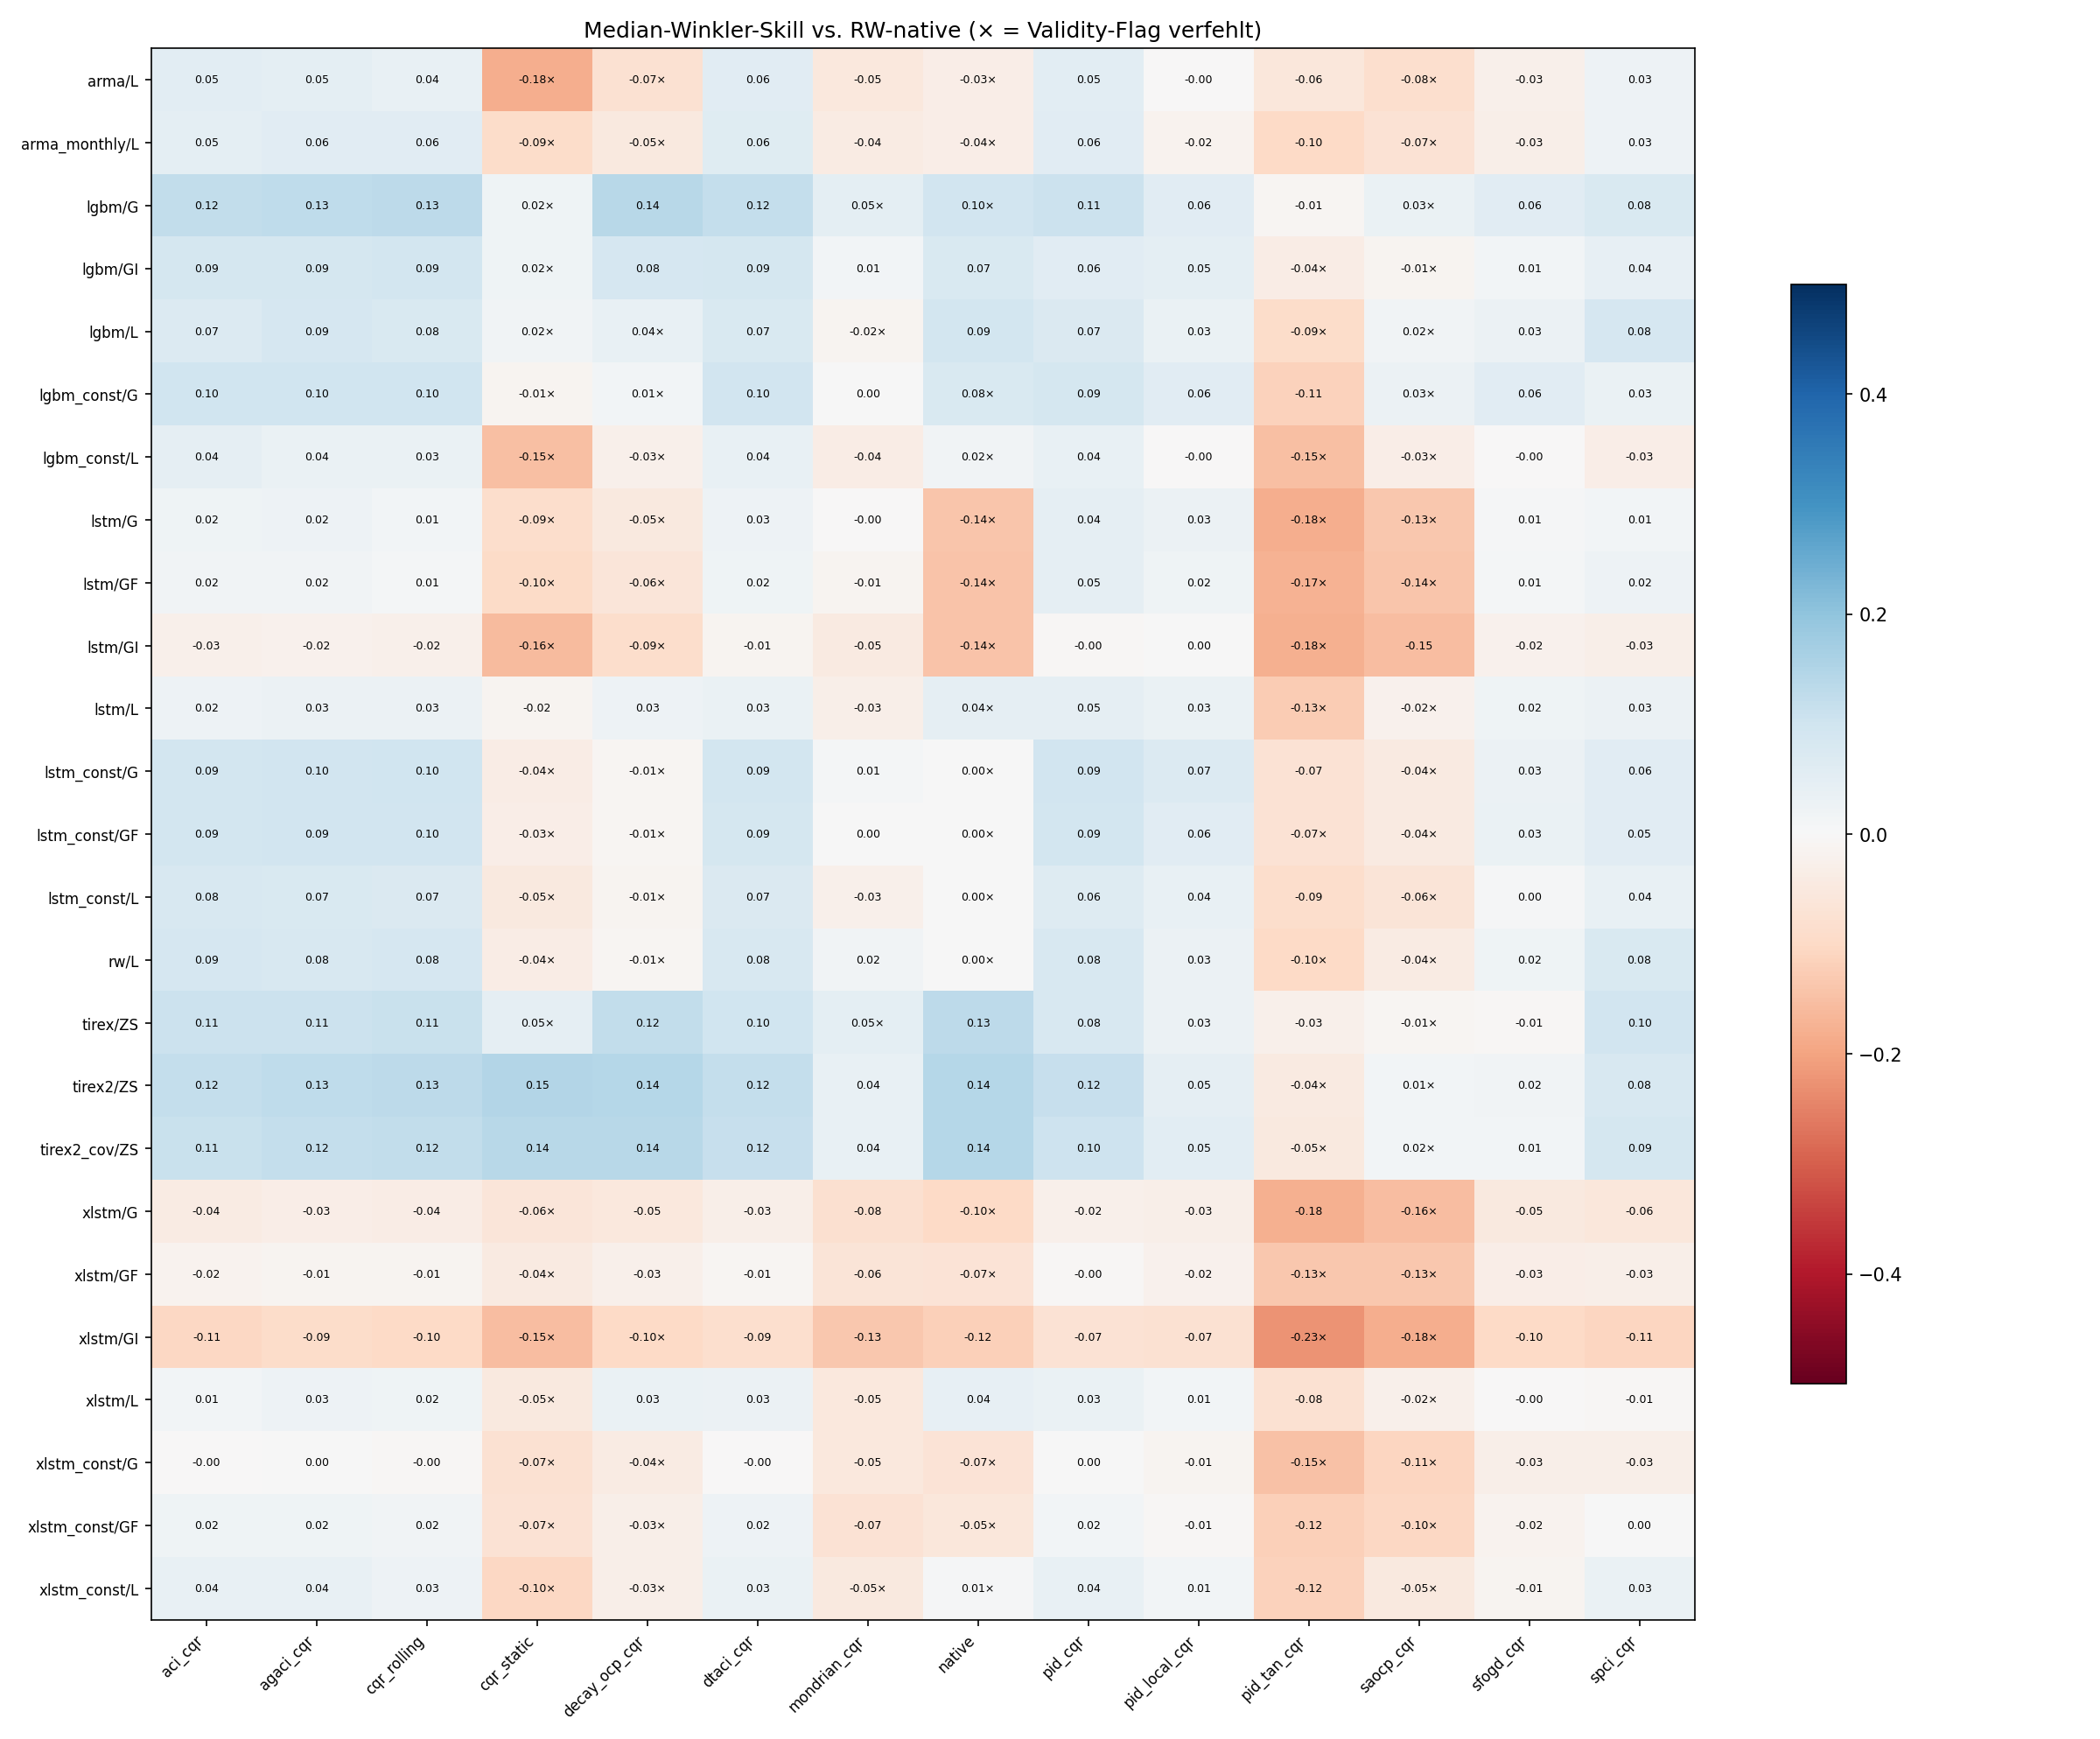
\includegraphics[width=1.15\textwidth]{figures/skill_heatmap.png}}
    \caption{Heatmap zur Übersicht der Modell-Skills.}
    \label{fig:skill_heatmap}
\end{figure}

% Das ist DAS Kernunterkapitel der Arbeit. Nimm dir hier am meisten Zeit.
%
% WAS HIER STEHT:
%  1. Das Ranking der besten validen Kombination je Modellfamilie
%     (tab:res_ranking unten, Zahlen eingetragen).
%  2. Die Kernaussage: das beste valide Paket ist ein ZERO-SHOT-
%     Foundation-Model ohne jedes Training auf diesen Daten
%     (tirex2/ZS), mit Winkler-Skill 0.146 gegen RW/L/native. Der beste
%     klassische Ansatz (rw/L/aci_cqr) kommt auf 0.085.
%     -> Ein Satz, der die Spannung benennt: dasselbe Modell, das bei der
%        Punktprognose exakt auf RW-Niveau liegt (8.2), erzeugt die mit
%        Abstand besten Intervalle. Der Vorsprung liegt vollstaendig in
%        der Form der praediktiven Verteilung, nicht in ihrem Zentrum.
%  3. Das xLSTM-Ergebnis EHRLICH aufschreiben. Das ist die namensgebende
%     Architektur der Arbeit und sie ist die SCHWAECHSTE Familie:
%     Median-Skill ueber alle Kombis -0.047 (letzter Platz), bestes
%     valides Paket xlstm/L/native mit 0.094 -- und das ausgerechnet mit
%     der nativen Quantilausgabe, also OHNE Nutzen aus der CP-Schicht.
%     Im GI-Regime ist der Skill negativ (-0.042).
%     -> Das nicht kleinreden. Ein negatives Kernergebnis, das sauber
%        gemessen wurde, ist wissenschaftlich wertvoller als ein
%        herbeigeredetes positives. In der Discussion aufgreifen:
%        277 Monate x 10 Laender sind schlicht zu wenig Daten fuer eine
%        Architektur dieser Kapazitaet.
%  4. !! ENTSCHEIDUNG -- COVERAGE VS. WINKLER (CLAUDE.md verbietet mir,
%     das fuer dich zu entscheiden):
%     Der Spitzenreiter tirex2/ZS/cqr_static hat Skill 0.1461, aber
%     mittlere Coverage 0.7496 -- also 5.0pp UNTER dem Ziel von 0.80 --
%     und passiert das Gate nur in 8 von 10 Laendern.
%     Der direkte Verfolger tirex2/ZS/decay_ocp_cqr hat Skill 0.1442
%     (0.0019 weniger, also 1.3% relativer Unterschied), aber Coverage
%     0.7866 und ist in 10 von 10 Laendern valide; mittlerer absoluter
%     Coverage-Abstand zum Ziel: 0.0279 gegenueber 0.0680 bei cqr_static.
%     DREI moegliche Auflösungen -- waehle EINE und begruende sie:
%       (a) cqr_static als Headline, decay_ocp als robustere Alternative
%           nennen. Maximiert die Schlagzeile, laedt aber den Vorwurf ein,
%           dass der Sieger unterdeckt.
%       (b) decay_ocp als Headline (Coverage-naeher, 100% Gate), cqr_static
%           als "hoechster Rohskill" in einem Nebensatz. Konservativ,
%           konsistent mit dem validity-first-Prinzip aus 7.1.
%       (c) Beide gemeinsam als "tirex2/ZS-Familie, Skill 0.14-0.15"
%           berichten und die Methodenwahl explizit als offen deklarieren.
%     MEINE EMPFEHLUNG: (b). Begruendung: du hast in 7.1 validity-first
%     als tragendes Prinzip vorregistriert. Wenn du dann die Kombination
%     mit dem groessten Coverage-Fehler zum Sieger kuerst, untergraebst du
%     dein eigenes Kriterium, und genau das wird ein Referee angreifen.
%     Aber es ist DEINE Entscheidung -- schreib sie explizit hin.

%  5. Ein Satz zur Streuung innerhalb tirex2: ueber die 14 CP-Methoden
%     reicht der Skill von -0.044 (pid_tan) bis 0.146 (cqr_static).
%     Die Wahl der Rekalibrierungsmethode ist also fuer das Ergebnis
%     ungefaehr so wichtig wie die Wahl des Modells. Das ist ein
%     eigenstaendiges Resultat und rechtfertigt den 14-Methoden-Vergleich.
%  6. Abbildung skill_heatmap.png einbinden (liegt in figures/).

%  7. WINKLER-DEKOMPOSITION UND TAIL-ASYMMETRIE -- NEU EINZUFUEGEN
%     2026-08-03. Diese Groessen sind in \cref{sec:eval:validity}
%     EINGEFUEHRT (Zerlegung in Breite, Unterschreitungs- und
%     Ueberschreitungs-Penalty, daraus die Tail-Asymmetrie), aber im
%     gesamten Ergebnisteil NICHT BERICHTET. Sie liegen fertig in
%     cells.csv (Spalten width, under_pen, over_pen, tail_asym).
%     Eine Metrik einzufuehren und dann nie zu verwenden ist eine
%     offene Flanke -- entweder hier berichten oder in 7.2 streichen.
%     Ich empfehle berichten: die Zahlen sagen etwas Nichttriviales.

Decomposing the Winkler score leads to the following results: The average interval width is 0.3301. The average penalty for the real value being under the interval is 0.0521 and the average penalty for the real value being over the interval is 0.0714. The width makes up $72.8\%$ of the average winkelr score. We conclude that the score is dominated by the sharpness of the intervals not by the violations. This explaines why a Model that is undercovering like $tirex2/cqr\_static$ is in the lead. The tail asymetry is the ratio of lower violations to all violations. On average over all cells it was 0.5059 with the median being 0.5. We conclude that they are basically symetical distributed. But the penalties are not. High violations cause an average penalty of 0.0715 while lower violations only cause an average penalty of 0.0521, that is a discrepancy of 37$\%$. We conclude that the likelihood of leaving the interval in each direction is the same, but if the next point is outside of the interval the high violations are expected to be further from the interval than the lower ones. This is consistent with the know right skewed ness of credit spreads. A symmetric CQR score cant learn these patterns. 
%     WAS ZU SCHREIBEN IST (ein Absatz, 4-6 Saetze):
%     (a) Woraus der Score besteht. Ueber die zulaessigen Kombinationen:
%           mittlere Breite        0.3301
%           Unterschreitungsstrafe 0.0521
%           Ueberschreitungsstrafe 0.0715
%         Die Breite macht 72.8% des mittleren Winkler-Scores aus.
%         -> Satz: der Score wird von der Schaerfe dominiert, nicht von
%            den Verletzungen. Das ist die Erklaerung dafuer, warum das
%            Ranking so stark mit der Intervallbreite korreliert und
%            warum ein leicht unterdeckendes Verfahren wie
%            tirex2/cqr_static ueberhaupt vorne landen kann.
%     (b) Die Tail-Asymmetrie (Anteil UNTERER an allen Verletzungen;
%         0.5 = symmetrisch). Ueber alle Zellen: Mittel 0.5049,
%         Median 0.5000 -- die Verletzungen sind der ANZAHL nach
%         praktisch symmetrisch verteilt.
%     (c) ABER: die Strafen sind es nicht (0.0715 oben gegen 0.0521
%         unten, also +37% Uebergewicht auf der Oberseite). Gleich viele
%         Verletzungen, aber die nach OBEN sind im Mittel deutlich
%         teurer.
%         -> Das ist der interessante Satz des Absatzes: wenn der Spread
%            aus dem Intervall laeuft, dann nach oben und weiter.
%            Oekonomisch plausibel (Spread-Ausweitungen sind sprunghaft,
%            Einengungen graduell) und konsistent mit der bekannten
%            Rechtsschiefe von Kreditspreads. NICHT als kausale Aussage
%            formulieren, sondern als Beobachtung, die zur bekannten
%            Verteilungsform passt.
%         -> Konsequenz benennen: ein SYMMETRISCHER CQR-Score kann diese
%            Asymmetrie strukturell nicht abbilden. Das ist ein
%            Kandidat fuer Future Work (asymmetrische oder
%            zweiseitig-getrennte Score-Familien) und gehoert in die
%            Discussion verlinkt.
%     (d) Ein Satz zur Modellordnung -- die klassischen Modelle sind am
%         staerksten unterseitig fehlgewichtet, die komplexen am
%         wenigsten. Nicht ueberinterpretieren, aber die Richtung ist
%         konsistent.
%
% ZAHLEN FUER PUNKT 7 (verifiziert, cells.csv, pool=rolling, nur
% validity_flag=True):
%   Tail-Asymmetrie je Modellfamilie (Mittel):
%     xlstm 0.483 | tirex2 0.510 | tirex2_cov 0.532 | lstm 0.533 |
%     lstm_const 0.540 | xlstm_const 0.540 | tirex 0.555 |
%     lgbm_const 0.577 | rw 0.604 | arma 0.608 | lgbm 0.611 |
%     arma_monthly 0.618
%   Tail-Asymmetrie je Land (Mittel) -- die groessere Streuung:
%     FI 0.431 | IT 0.444 | BE 0.502 | FR 0.504 | AT 0.551 | NL 0.552 |
%     ES 0.567 | PT 0.572 | GR 0.594 | IE 0.642
%     -> Spanne 0.43 bis 0.64. Die Laenderheterogenitaet ist groesser als
%        die Modellheterogenitaet. Passt zum Kendall-Befund in 8.9
%        (tau 0.346) und stuetzt die dortige Aussage von einer anderen
%        Seite -- diese Verbindung explizit ziehen, sie ist gratis.
%   Tail-Asymmetrie je CP-Methode (Mittel, nur zulaessige Kombis):
%     cqr_static 0.471 | mondrian 0.522 | decay_ocp 0.522 |
%     sfogd 0.528 | dtaci 0.529 | pid 0.530 | pid_local 0.533 |
%     cqr_rolling 0.536 | saocp 0.540 | aci 0.540 | agaci 0.543 |
%     spci 0.553 | native 0.556 | pid_tan 0.562
%     -> Spannweite nur 0.47-0.56: die Wahl der CP-Methode veraendert die
%        Asymmetrie kaum. Das ist ein NICHT-Befund und genau deshalb
%        berichtenswert: die Rekalibrierungsschicht korrigiert das
%        Niveau der Coverage, aber nicht ihre Schiefe. Ein Satz.
The tail asymmetrie between all conformal prediction modells ranges from 0.47 to 0.56. This shows that the CP only correct for the coverage but not the symmetrie. 
% ZITATE fuer Punkt 7: winkler1972, gneiting2007 (Zerlegung properer
%   Scores), romano2019cqr (Symmetrie des CQR-Scores als strukturelle
%   Grenze).
%
% ZAHLEN (verifiziert, ranking_all.csv, nur validity_flag=True):
%   Bestes valides Paket je Modellfamilie:
%     tirex2/ZS/cqr_static        skill 0.1461  cov 0.750  gate 0.8
%     tirex2_cov/ZS/native        skill 0.1409  cov 0.839  gate 0.8
%     lgbm/G/decay_ocp_cqr        skill 0.1394  cov 0.824  gate 0.7
%     tirex/ZS/native             skill 0.1327  cov 0.813  gate 1.0
%     lstm_const/G/agaci_cqr      skill 0.1107  cov 0.798  gate 1.0
%     lgbm_const/G/cqr_rolling    skill 0.0989  cov 0.829  gate 1.0
%     xlstm/L/native              skill 0.0939  cov 0.817  gate 0.7
%     rw/L/aci_cqr                skill 0.0852  cov 0.812  gate 1.0
%     xlstm_const/L/spci_cqr      skill 0.0717  cov 0.756  gate 1.0
%     lstm/L/pid_cqr              skill 0.0621  cov 0.810  gate 1.0
%     arma_monthly/L/dtaci_cqr    skill 0.0612  cov 0.809  gate 1.0
%     arma/L/dtaci_cqr            skill 0.0584  cov 0.813  gate 1.0
%   Median-Skill ueber ALLE Kombis je Familie (auch invalide):
%     tirex2 0.118 | tirex2_cov 0.108 | tirex 0.088 | lgbm 0.063 |
%     lstm_const 0.037 | lgbm_const 0.032 | rw 0.025 | lstm -0.005 |
%     arma -0.014 | xlstm_const -0.020 | arma_monthly -0.023 | xlstm -0.047
%   tirex2 ueber alle 14 CP-Methoden (Skill / Coverage / Gate-Anteil):
%     cqr_static 0.146/0.750/0.8  decay_ocp 0.144/0.787/1.0
%     native 0.142/0.855/0.7      cqr_rolling 0.132/0.794/1.0
%     agaci 0.126/0.797/1.0       aci 0.121/0.799/1.0
%     dtaci 0.120/0.806/1.0       pid 0.116/0.800/1.0
%     spci 0.080/0.762/1.0        pid_local 0.046/0.802/1.0
%     mondrian 0.035/0.856/0.9    sfogd 0.017/0.801/0.8
%     saocp 0.012/0.894/0.3 (INVALIDE)  pid_tan -0.044/0.810/0.6 (INVALIDE)
%   Bestes valides xlstm-Paket je Regime:
%     L/native 0.0939 | GF/cqr_rolling 0.0098 | G/pid_cqr -0.0070
%     | GI/native -0.0423
%   Skill je Land (valide Kombis, Median): IE 0.231 | PT 0.191 | GR 0.120
%     | ES 0.095 | BE 0.051 | NL -0.002 | AT -0.015 | FR -0.047
%     | FI -0.052 | IT -0.070
%     -> Zwei Saetze wert: der Skill ist stark laenderabhaengig, und
%        ausgerechnet in Italien (dem groessten Markt) verliert das Feld
%        im Median gegen den Random Walk.
%
% ZITATE: winkler1972, gneiting2007, gneiting2007sharpness,
%   podest2026tirex2, auer2025tirex, beck2024xlstm.
%
% >>> THESIS-ONLY >>>
% - Vollstaendige Ranking-Tabelle aller 485 validen Kombinationen in den
%   Anhang (ranking_all.csv, gefiltert auf validity_flag).
% - Absatz zur Frage, warum ZS so gut abschneidet: keine Schaetzunsicherheit
%   in den Parametern, weil nichts geschaetzt wird; die praediktive
%   Verteilung kommt aus einem auf Millionen Zeitreihen vortrainierten
%   Modell. Gegenargument sauber dagegenstellen: Kontaminationsverdacht
%   (Release 2026-07-01, Cutoff undokumentiert, Testfenster bis 2026-04)
%   -> Verweis auf Limitations.
% - Per-Land-Aufschluesselung der Top-3-Pakete.
% <<< THESIS-ONLY <<<
%
% [arXiv-Kuerzung]: tab:res_ranking + skill_heatmap + 2 Absaetze
%   (Headline + xLSTM-Negativergebnis). Der Laender-Schnitt in 1 Satz.
The zero shot models where pretrained on millions of time series data and gained their predictive distribution that way. It is possible that the model already saw the date we are working with in this pre training, since the TiRex2 Model was released in 2026-07-01 and our testing window until 2026-04. More about that in \cref{sec:res:limitations}.\\
In Table ~\ref{tab:res_percountry} we how the top 3 packages and the best classical benchmark perform on all 10 counties. All Models represented in the Table reach the highest skill on Ireland. While the top three Models reach the lowest skill on Finland the classical method reaches its lowest skill on Italy (-0.049). None of the top three Models have a negative skill in any countrie. The classical package is the only one out of the 4 to be admissible on all 10 countries. 

\begin{table}[t]
\centering
\caption{% TODO Caption. Best admissible package per model family, ranked
         by median Winkler skill against RW/L/native.         Under a stricter, post hoc gate requiring all ten countries,
         four of the twelve selections change: \texttt{tirex2} to
         \texttt{decay\_ocp\_cqr} (0.144), \texttt{tirex2\_cov} to
         \texttt{decay\_ocp\_cqr} (0.139), \texttt{lgbm} to
         \texttt{agaci\_cqr} (0.128), and \texttt{xlstm} to
         \texttt{cqr\_rolling} (0.068); the remaining eight are
         unchanged. The ordering of the leading group is unaffected, but
         \texttt{xlstm} then ranks below the random walk.}
\label{tab:res_ranking}
\begin{tabular}{llccc}
\toprule
Model & Regime / method & Median skill & Mean coverage & Admissible countries \\
\midrule
\texttt{tirex2}        & ZS / \texttt{cqr\_static}     & 0.146 & 0.750 & 8/10 \\
\texttt{tirex2\_cov}   & ZS / \texttt{native}          & 0.141 & 0.839 & 8/10 \\
\texttt{lgbm}          & G / \texttt{decay\_ocp\_cqr}  & 0.139 & 0.824 & 7/10 \\
\texttt{tirex}         & ZS / \texttt{native}          & 0.133 & 0.813 & 10/10 \\
\texttt{lstm\_const}   & G / \texttt{agaci\_cqr}       & 0.111 & 0.798 & 10/10 \\
\texttt{lgbm\_const}   & G / \texttt{cqr\_rolling}     & 0.099 & 0.829 & 10/10 \\
\texttt{xlstm}         & L / \texttt{native}           & 0.094 & 0.817 & 7/10 \\
\texttt{rw}            & L / \texttt{aci\_cqr}         & 0.085 & 0.812 & 10/10 \\
\texttt{xlstm\_const}  & L / \texttt{spci\_cqr}        & 0.072 & 0.756 & 10/10 \\
\texttt{lstm}          & L / \texttt{pid\_cqr}         & 0.062 & 0.810 & 10/10 \\
\texttt{arma\_monthly} & L / \texttt{dtaci\_cqr}       & 0.061 & 0.809 & 10/10 \\
\texttt{arma}          & L / \texttt{dtaci\_cqr}       & 0.058 & 0.813 & 10/10 \\
\bottomrule
\end{tabular}
\end{table}

\begin{table}[t]
\centering
\caption{% TODO Caption. All 14 recalibration methods applied to
         \texttt{tirex2}/ZS. Skill is the median Winkler skill against
         RW/L/\texttt{native}; $\dagger$ marks combinations that fail the
         admissibility gate.}
\label{tab:res_tirex2_cp}
\begin{tabular}{lccc}
\toprule
Method & Median skill & Mean coverage & Admissible countries \\
\midrule
\texttt{cqr\_static}     & 0.146 & 0.750 & 8/10 \\
\texttt{decay\_ocp\_cqr} & 0.144 & 0.787 & 10/10 \\
\texttt{native}          & 0.142 & 0.855 & 7/10 \\
\texttt{cqr\_rolling}    & 0.132 & 0.794 & 10/10 \\
\texttt{agaci\_cqr}      & 0.126 & 0.797 & 10/10 \\
\texttt{aci\_cqr}        & 0.121 & 0.799 & 10/10 \\
\texttt{dtaci\_cqr}      & 0.120 & 0.806 & 10/10 \\
\texttt{pid\_cqr}        & 0.116 & 0.800 & 10/10 \\
\texttt{spci\_cqr}       & 0.080 & 0.762 & 10/10 \\
\texttt{pid\_local\_cqr} & 0.046 & 0.802 & 10/10 \\
\texttt{mondrian\_cqr}   & 0.035 & 0.856 & 9/10 \\
\texttt{sfogd\_cqr}      & 0.017 & 0.801 & 8/10 \\
\texttt{saocp\_cqr}$^\dagger$    & 0.012 & 0.894 & 3/10 \\
\texttt{pid\_tan\_cqr}$^\dagger$ & $-0.044$ & 0.810 & 6/10 \\
\bottomrule
\end{tabular}
\end{table}

\begin{table}[t]
\centering\small
\caption{% TODO Caption. Per-country skill and coverage of the three
         leading packages and of the best classical benchmark. Skill is
         relative to RW/L/\texttt{native} of the same country; coverage
         target is 0.80. $\dagger$ marks a country in which the
         calibration null is rejected (FDR $q<0.10$), i.e.\ a cell that
         fails the admissibility gate.}
\label{tab:res_percountry}
\begin{tabular}{lcccccccc}
\toprule
& \multicolumn{2}{c}{\texttt{tirex2}/ZS} & \multicolumn{2}{c}{\texttt{tirex2\_cov}/ZS} & \multicolumn{2}{c}{\texttt{lgbm}/G} & \multicolumn{2}{c}{\texttt{rw}/L} \\
& \multicolumn{2}{c}{\texttt{cqr\_static}} & \multicolumn{2}{c}{\texttt{native}} & \multicolumn{2}{c}{\texttt{decay\_ocp\_cqr}} & \multicolumn{2}{c}{\texttt{aci\_cqr}} \\
\cmidrule(lr){2-3}\cmidrule(lr){4-5}\cmidrule(lr){6-7}\cmidrule(lr){8-9}
Country & Skill & Cov. & Skill & Cov. & Skill & Cov. & Skill & Cov. \\
\midrule
AT & 0.103 & 0.811 & 0.097 & 0.819 & 0.120 & 0.780 & $0.002$ & 0.835 \\
BE & 0.190 & 0.835 & 0.185 & 0.835 & 0.159 & 0.898$^\dagger$ & 0.148 & 0.795 \\
ES & 0.212 & 0.780 & 0.206 & 0.787 & 0.174 & 0.843 & 0.180 & 0.827 \\
FI & 0.013 & 0.772 & 0.008 & 0.843 & 0.010 & 0.795 & $-0.027$ & 0.819 \\
FR & 0.026 & 0.740 & 0.033 & 0.827 & 0.014 & 0.772 & $-0.006$ & 0.780 \\
GR & 0.336 & 0.780 & 0.315 & 0.898$^\dagger$ & 0.192 & 0.882$^\dagger$ & 0.196 & 0.858 \\
IE & 0.410 & 0.598$^\dagger$ & 0.444 & 0.858 & 0.272 & 0.835 & 0.386 & 0.748 \\
IT & 0.017 & 0.780 & 0.023 & 0.803 & 0.008 & 0.748 & $-0.049$ & 0.803 \\
NL & 0.064 & 0.843 & 0.068 & 0.819 & 0.039 & 0.772 & 0.022 & 0.819 \\
PT & 0.248 & 0.559$^\dagger$ & 0.295 & 0.898$^\dagger$ & 0.243 & 0.913$^\dagger$ & 0.318 & 0.835 \\
\midrule
Median / mean & 0.146 & 0.750 & 0.141 & 0.839 & 0.139 & 0.824 & 0.085 & 0.812 \\
Admissible & \multicolumn{2}{c}{8/10} & \multicolumn{2}{c}{8/10} & \multicolumn{2}{c}{7/10} & \multicolumn{2}{c}{10/10} \\
\bottomrule
\end{tabular}
\end{table}


%------------------------------------------------------------------------
\subsection{RQ3: does the conformal layer pay off?}
\label{sec:res:rq3}
%------------------------------------------------------------------------
We wanted to find out wether the CP calibration methods led to an imporvement in performance when compared to the native quantile output of the Models. The answer is yes but only for the adaptive online CP methods with a moderate effect. The seven winning methods have a $d\_norm$ ranging from -0.054 to -0.031 with Pantel-t between -4 and -2. Three Methods performe worse thatn the native: $cqr\_static (+0.027), saocp (+0.052),pid\_tan (+0.102)$. The conformal layer is no miracle remedy that always works. The most important effect is not the skill but the validity. Native Model output only passes the Gate in 13.3$\%$ of cases while $dtaci/pid/pid\_local/sfogd/spci$ pass in $100\%$ of cases. We conclude that the mains trength of the conformal method is calibrating to the wanted coverage and not so much sharpness. After the FDR correction the rate of winning Models ranges only from 0.37 to 0.50. On 10 correlated countries and 127 Months this is a consistent but not overwhelming signal.
% WAS HIER STEHT:
%  1. Die Frage klar stellen: bringt eine Rekalibrierungsmethode gegenueber
%     der nativen Quantilausgabe des Modells einen messbaren Vorteil?
%     Kontrastfamilie RQ3 mit 689 Kontrasten, eigene BH-FDR-Familie.
%  2. Antwort: JA, aber nur fuer die adaptiven Online-Verfahren, und der
%     Effekt ist moderat. Die sieben Gewinner-Methoden liegen bei
%     d_norm zwischen -0.054 und -0.031 (negativ = besser als native),
%     mit Panel-t zwischen -4.0 und -2.0.
%  3. Die Kehrseite ausdruecklich nennen: drei Methoden sind SCHLECHTER
%     als native -- cqr_static (+0.027), saocp (+0.052) und vor allem
%     pid_tan (+0.102). Die CP-Schicht ist also kein Selbstlaeufer.
%  4. Der wichtigere Effekt ist nicht der Skill, sondern die VALIDITAET:
%     native passiert das Gate nur in 13.2% der Faelle, dtaci/pid/
%     pid_local/sfogd/spci in 100%. Formuliere das als die eigentliche
%     Antwort auf RQ3: der Gewinn der CP-Schicht ist primaer Kalibrierung,
%     sekundaer Schaerfe. Das passt exakt zum validity-first-Prinzip.
%  5. Ein Satz Vorsicht: die Anteile FDR-signifikanter Laender liegen bei
%     den Gewinnern nur zwischen 0.37 und 0.50 (Median ueber Kontraste).
%     Bei 10 korrelierten Laendern und 127 Monaten ist das ein
%     konsistentes, aber kein ueberwaeltigend starkes Signal.
%
% ZAHLEN (verifiziert, dm_contrasts.csv, rq=="RQ3", Median ueber die
%   53 Kontraste je Methode; d_norm negativ = Methode besser als native):
%   Methode         d_norm   share_a_better  Panel-t   share_sig_FDR
%   dtaci_cqr       -0.054       0.7          -3.72        0.43
%   pid_cqr         -0.054       0.8          -3.97        0.50
%   aci_cqr         -0.047       0.6          -3.46        0.40
%   cqr_rolling     -0.045       0.6          -3.21        0.37
%   agaci_cqr       -0.043       0.6          -3.55        0.47
%   spci_cqr        -0.038       0.6          -2.01        0.40
%   pid_local_cqr   -0.031       0.7          -2.95        0.37
%   sfogd_cqr       -0.008       0.5          -1.61        0.30
%   decay_ocp_cqr   +0.002       0.5          -0.36        0.47
%   mondrian_cqr    +0.023       0.5          -0.66        0.47
%   cqr_static      +0.027       0.3          +8.74        0.67
%   saocp_cqr       +0.052       0.0          +4.03        0.43
%   pid_tan_cqr     +0.102       0.3          +1.95        0.77
%   Gesamtmedian RQ3: d_norm -0.0034, share_a_better 0.50, t -1.27
%     -> WICHTIG: ueber ALLE Methoden gemittelt ist der Effekt fast null.
%        Erst die Aufspaltung nach Methode zeigt das Bild. Genau so
%        schreiben, nicht den Gesamtmedian verschweigen.
%
% ZITATE: romano2019cqr, gibbs2021aci, gibbs2024dtaci, zaffran2022agaci,
%   angelopoulos2023pid, xu2023spci, bhatnagar2023sfogd,
%   angelopoulos2024decay, vovk2003mondrian, dieboldmariano1995,
%   harvey1997, newey1987, benjamini1995fdr.
%
% [arXiv-Kuerzung]: 1 Absatz + die RQ3-Spalte in einer kombinierten
%   Kontrasttabelle mit RQ1/RQ2.
\begin{table}[htbp]
  \centering
  \caption{Results for RQ3: Comparison of CP methods against native model output (median across 53 contrasts per method). Negative $d_{\text{norm}}$ indicates superiority of the CP method.}
  \label{tab:rq3_results}
  \begin{tabular}{l c c c c}
    \toprule
    \textbf{Method} & $d_{\text{norm}}$ & \textbf{Share } $A > \text{native}$ & \textbf{Panel } $t$ & \textbf{Share Sig. (FDR)} \\
    \midrule
    \texttt{dtaci\_cqr}     & $-0.054$ & $0.7$ & $-3.72$ & $0.43$ \\
    \texttt{pid\_cqr}       & $-0.054$ & $0.8$ & $-3.97$ & $0.50$ \\
    \texttt{aci\_cqr}       & $-0.047$ & $0.6$ & $-3.46$ & $0.40$ \\
    \texttt{cqr\_rolling}   & $-0.045$ & $0.6$ & $-3.21$ & $0.37$ \\
    \texttt{agaci\_cqr}     & $-0.043$ & $0.6$ & $-3.55$ & $0.47$ \\
    \texttt{spci\_cqr}      & $-0.038$ & $0.6$ & $-2.01$ & $0.40$ \\
    \texttt{pid\_local\_cqr}& $-0.031$ & $0.7$ & $-2.95$ & $0.37$ \\
    \midrule
    \texttt{sfogd\_cqr}     & $-0.008$ & $0.5$ & $-1.61$ & $0.30$ \\
    \texttt{decay\_ocp\_cqr}& $+0.002$ & $0.5$ & $-0.36$ & $0.47$ \\
    \texttt{mondrian\_cqr}  & $+0.023$ & $0.5$ & $-0.66$ & $0.47$ \\
    \midrule
    \texttt{cqr\_static}    & $+0.027$ & $0.3$ & $+8.74$ & $0.67$ \\
    \texttt{saocp\_cqr}     & $+0.052$ & $0.0$ & $+4.03$ & $0.43$ \\
    \texttt{pid\_tan\_cqr}   & $+0.102$ & $0.3$ & $+1.95$ & $0.77$ \\
    \midrule
    \textbf{Overall Median RQ3} & $-0.0034$ & $0.50$ & $-1.27$ & -- \\
    \bottomrule
  \end{tabular}
\end{table}

%------------------------------------------------------------------------
\subsection{RQ1: pooling across countries and fine-tuning}
\label{sec:res:rq1}
%------------------------------------------------------------------------
We wanted to find out if one global Model for all countries out performes one lokal Model for each country. In Table ~\ref{tab:rq1_results} we see that the Global (G) vs. the Lokal (L) regime has a positive $d\_norm$ indicating a superiority of the L Regime. LSTM and xLSTM loose performance while lightGBM is the only one gaining performance with pooling. One possible explanation for this is that the Neural Nets are sensitive to different scales and uneven variance between countrie data. Our spreads range from 0.201 in the Netherlands to 1.907 in Greece a multiple of about 9.5 and the variance ranges from 0.042 in the Netherlands to 0.372 in Grecce a multiple of about 8.8. While lgbm is trained on the same data and sees an imporvment in performance with pooling.  \\
In the comparison GF vs. G, so finetuned after global training vs. just global training the fine tuned models had an overal, but not statistically significant, better performance with a $d\_norm$ of -0.006. This is a small but consistent advantage $(share\_a\_better 0.60)$. While xLSTM profits from finetuning ( $d\_norm$ -0.021)LSTM doesn't really see a change ($d\_norm$+0.0014). \\
We see the strongest effect in the comparisson GF vs. GI with the $d\_norm$ being -0.0543 and $share\_a\_better=0.90$. It has a a Panel-t test of -3.33 which proves an average effect, but the Median q of 0.245 show that the effect is not statistically significant per country after correction. So the the finetuning regime beats the country specific bias correction regime consistently, this shows that fine tuning does more than an intercept shift. The $d\_norms$ for xLSTM is -0.06 with a consistent $share\_a\_better$ of 0.9, the largest Panel t (-4.93), the lowest Median q (0.145) and full seed stability. This shows that correctiong for a bias in the global model is inferior to fine tuning the global model. \\
The comparisson GF vs. L was added post hoc, with a $d\_norm$ of 0.016, solidifies L as the consistent winner and is consistent with the results of G vs. L and GF vs. G. L beat GF $60\%$ of times but with a Panel t of 0.86 abd a Median q of 0.527 not statistically significant. We also see a low seed stability in the Model contrasts (LSTM 0.43, xLSTM 0.21).\\
The Zero shot regime reach the highest gate rate with 0.833 followed by the Lokal regime with 0.668 as can be seen in Table ~\ref{tab:rq1_results}. Regime GI has the lowest gate rate with 0.602. The average skill in all admissable cells is also led by the zero shot regime with 0.11 again followed by the local regime with 0.021. In generell we see here the same order as with the gating rate. The worst performer was again the GI Regime with -0.037.\\



%
% --- K1: SACHFEHLER, MUSS RAUS ------------------------------------
% Der Satz "So the finetuning regime beats the country embedding regime"
% ist FALSCH. GI ist NICHT das Embedding-Regime.
%   Das Laender-Embedding steckt bereits in G. \cref{sec:exp:regimes}:
%   "The country identity is passed to the model, as a learned embedding
%   for the neural networks and as a native categorical feature for
%   LightGBM." -- das steht unter dem G-Punkt.
%   GI = G PLUS additiver Intercept-Shift (rollierender Median der letzten
%   <=36 realisierten OOS-Residuen, Parallelshift auf alle drei Quantile,
%   Breite unveraendert; \cref{sec:conformal:derived}, eq:gplusi).
%
% DIE RICHTIGE FRAMUNG -- und sie ist schaerfer als deine:
%   G hat das Embedding bereits. Also fragen die beiden Kontraste:
%     GF vs G  : bringt Gewichts-Fine-Tuning etwas UEBER das Embedding
%                hinaus?  -> ja, aber wenig (-0.006)
%     GF vs GI : von den beiden Wegen, ZUSAETZLICHE Laenderspezifik
%                aufzusetzen -- Gewichte anpassen oder Niveau
%                verschieben -- welcher ist besser?  -> Gewichte, klar
%                (-0.054)
%   Dein naechster Satz ("correcting for a bias in the global model is
%   inferior to fine tuning") ist bereits richtig -- nur der Satz davor
%   widerspricht ihm. Streich ihn und schreib die Framung oben hin.
%
% --- E1: SIGNIFIKANZ FEHLT IM GANZEN ABSCHNITT --------------------
% Du schreibst "not statistically significant" nur bei G vs L. Das gilt
% fuer ALLE Kontraste und muss einmal zentral gesagt werden.
%   KEIN EINZIGER RQ1-Kontrast ist auf Kontrastebene FDR-signifikant.
%   Von 266 vorregistrierten Kontrasten haben 30 ein median-q < 0.10,
%   das kleinste q ueberhaupt ist 0.019.
%   Median-q je Kontrasttyp: G vs L 0.413 | GF vs G 0.403 | GF vs GI 0.245
%   Gleichzeitig haben 131 von 266 ein |Panel-t| > 1.96.
%   -> DIESE DISKREPANZ MUSST DU ERKLAEREN, sonst wirkt die Tabelle
%      widerspruechlich: der Panel-t fragt "ist der Effekt im Mittel
%      ueber die Laender vorhanden?", der q-Wert "ist er innerhalb
%      einzelner Laender nach Korrektur nachweisbar?". Bei zehn Laendern
%      und 127 Monaten faellt die zweite Frage negativ aus.
%   -> Formuliere alle drei Befunde konsequent als GERICHTET, nicht als
%      signifikant. "consistently favours X" statt "significantly better".
%
% --- E2: SEED-STABILITAET -- verstaerkt deinen Hauptbefund ---------
% Fehlt komplett, ist aber die Absicherung deines staerksten Ergebnisses.
%   GF vs GI, Anteil seed-vorzeichenstabiler Kontraste:
%     xlstm 1.00 (14 von 14)  |  lstm 0.14 (2 von 14)
%   -> xlstm/GF vs GI ist der EINZIGE RQ1-Kontrast, der ueber alle drei
%      Seeds vollstaendig richtungsstabil ist -- und gleichzeitig der mit
%      dem groessten Effekt (-0.060), dem staerksten Panel-t (-4.93) und
%      dem kleinsten q (0.145). Das ist dein belastbarster RQ1-Befund,
%      und du solltest ihn genau so auszeichnen.
%   -> Die LSTM-Version desselben Kontrasts ist mit 0.14 fast durchgehend
%      instabil. Nach diagnostics_foundation.txt Paragraph 4.4 darf fuer
%      sie KEINE Rangaussage getroffen werden. Also: der Befund traegt
%      ueber xLSTM, nicht ueber LSTM. Ehrlich hinschreiben.
%   Zum Vergleich G vs L: lstm 0.29, xlstm 0.57 -- beide schwach.
%
% --- E3: NEUER KONTRAST GF vs L (post hoc, 2026-08-03) -------------
% Schliesst die Luecke, die deinen Abschnitt bisher unvollstaendig laesst.
%   Bisher: aus G vs L folgt L > G, aus GF vs G folgt GF > G. Die Ordnung
%   zwischen L und GF war UNBESTIMMT -- der vorregistrierte Kontrastsatz
%   enthaelt kein GF vs L. Jetzt gerechnet, gleiche Maschinerie
%   (DM/HLN je Land, df=126, Common Sample, Panel-t NW Lag 3), EIGENE
%   BH-FDR-Familie (84 Kontraste, 840 Zellen), damit die q-Werte der
%   vorregistrierten Kontraste unveraendert bleiben.
%   ZAHLEN: d_norm +0.016 | share_a 0.40 | Panel-t +0.86 | median q 0.527
%           | FDR-sig 0.13 | 6 von 84 mit q<0.10, kleinstes q 0.083
%           je Modell: lstm +0.016 (seed-stabil 0.43),
%                      xlstm +0.014 (seed-stabil 0.21)
%   -> GF bleibt also HINTER L. Die Kette ist damit in sich stimmig:
%        Pooling kostet        +0.017
%        Fine-Tuning holt      -0.006 zurueck
%        Rueckstand auf L      +0.016 bleibt
%      (Mediane addieren sich nicht exakt; 0.017-0.006=0.011 gegen
%       gemessene 0.016 ist konsistent, nicht identisch -- so schreiben.)
%   -> SCHWACH: median q 0.527, seed-instabil. Formuliere ihn als
%      "the local model remains ahead, though the difference is small and
%      not statistically distinguishable" -- als Richtungsbestaetigung,
%      nicht als Beleg.
%   !! MUSS DEKLARIERT WERDEN: dagger in tab:rq1_results, Amendment in
%      diagnostics_foundation.txt Paragraph 11, und Eintrag in der
%      Post-hoc-Liste in limitations.tex 9.8 Punkt 5 (wird der vierte).
%
% --- E4: DEINE HYPOTHESE HAT EIN GEGENARGUMENT ---------------------
% Du schreibst "Neural Nets are sensitive to different scales and uneven
% variance between countries". Das ist eine gute Hypothese und richtig
% als solche gekennzeichnet. Zwei Dinge fehlen:
%   (a) BELEG DER PRAEMISSE. Die Heterogenitaet ist real und quantifizierbar
%       (Testfenster, Level-Skala, aus dem RW-Stream):
%         Spread-Niveau (Median je Land): NL 0.201 ... GR 1.907  -> 9.5x
%         Volatilitaet (sd der Aenderungen): NL 0.042 ... GR 0.372 -> 8.8x
%       Diese zwei Zahlen gehoeren in den Satz, sonst ist die Hypothese
%       unbelegt behauptet.
%   (b) DAS GEGENARGUMENT, das du selbst bringen musst: LightGBM sieht
%       EXAKT dieselbe Heterogenitaet und gewinnt trotzdem durch Pooling
%       (-0.014). Skalenheterogenitaet allein kann den Befund also nicht
%       erklaeren -- sonst muesste LightGBM ebenfalls verlieren. Die
%       Erklaerung muss architekturspezifisch sein (z.B. dass Baeume
%       ueber die kategoriale Laendervariable splitten koennen, waehrend
%       das NN-Embedding bei 277 Monaten x 10 Laendern zu wenig Signal
%       bekommt). Als HYPOTHESE kennzeichnen -- das Design testet sie nicht.
%   -> Ein Absatz, der die eigene Erklaerung gleich selbst relativiert,
%      ist deutlich stark. Nicht weglassen.
%
% --- E5: PANEL C KOMMT IM TEXT GAR NICHT VOR -----------------------
% Zwei bis drei Saetze, sie sind billig und schliessen den Abschnitt:
%   Gate-Rate je Regime : L 0.668 > G 0.643 > GF 0.631 > GI 0.602
%   Median-Skill (nur zulaessige Kombis):
%                         L +0.031 > G +0.014 > GF +0.010 > GI -0.037
%   -> BEIDE ACHSEN ORDNEN DIE REGIME IDENTISCH. Je mehr kuenstliche
%      Laenderspezifik auf das globale Modell aufgesetzt wird, desto
%      schlechter wird sowohl die Kalibrierbarkeit als auch der Skill.
%      GI ist auf beiden Achsen letzter -- was konsistent damit ist,
%      dass es eine Guardrail ist und kein ernsthafter Kandidat.
%   -> ZS steht mit Gate 0.833 und Skill +0.110 deutlich vor allem
%      anderen, gehoert hier aber nur als Verweis auf 8.3 hin, nicht
%      als RQ1-Befund (RQ1 vergleicht nur trainierte Regime).
%
% --- E6: VERBINDUNG ZU 8.3 ----------------------------------------
% Ein Satz, der den Bogen schlaegt und zugleich ehrlich ist:
%   Das beste valide xlstm-Paket ist xlstm/L/native (0.094) -- das
%   Ranking bestaetigt also, was die Kontraste sagen.
%   ABER: dieser Eintrag ist der schwaechste der ganzen Ranking-Tabelle.
%   Er besteht das Gate in 7 von 10 Laendern, er ist nur fuer EINEN von
%   drei Seeds zulaessig (Seed 44: 0.094; Seed 42: 0.043 und Seed 43:
%   -0.008 fallen beide durch), und seine Seed-Spanne (0.102) uebersteigt
%   den eigenen Skill (0.094).
%   -> Das schwaecht deinen Befund NICHT, es staerkt ihn: selbst die
%      beste xLSTM-Konfiguration ist fragil. Und es gehoert nach 8.3
%      Punkt 3 verlinkt, wo du das xLSTM-Negativergebnis ehrlich
%      berichtest.
The best valid xlstm package is xlstm/L/native (0.094) even though it only passes the validity gate in 7/10 counties and is only admissible vor one out of the three seeds (Seed 44: 0.094; Seed 42: 0.043 und Seed 43: -0.008) . The ranking verifies the results of the contrasts. 
% --- STRUKTURVORSCHLAG fuer den ergaenzten Abschnitt ---------------
%   Absatz 1  G vs L        (steht, + E4a/E4b ergaenzen)
%   Absatz 2  GF vs G       (steht, + K1-Framung: was Embedding, was FT)
%   Absatz 3  GF vs GI      (steht, K1 korrigieren, + E2 Seed-Stabilitaet)
%   Absatz 4  GF vs L       (NEU, E3)
%   Absatz 5  Regime-Ebene + Verbindung zu 8.3   (NEU, E5 + E6)
%   Absatz 6  Signifikanz-Caveat fuer alle vier Kontraste  (NEU, E1)
%             -- ans ENDE, damit es den Abschnitt rahmt statt ihn
%                gleich am Anfang zu entwerten.
% =====================================================================
%
% ZITATE: beck2024xlstm, hochreiter1997lstm, ke2017lightgbm.
%
% [arXiv-Kuerzung]: 1 Absatz, die drei Kontraste als Zahlentripel im Satz.
\begin{table}[htbp]
  \centering\small
  \caption{Results for RQ1 (pooling and fine-tuning). \textbf{Panels A and B}
  report normalised Diebold--Mariano loss differentials
  $d_{\text{norm}}=\bar d/\bar W^{\text{ref}}$ with $d_t=W_t^{A}-W_t^{B}$,
  aggregated as the median over the ten countries; a \emph{negative} value
  means A has the lower loss, i.e.\ A is better. \textbf{Panel C} reports
  the median Winkler skill $1-\bar W/\bar W^{\text{ref}}$, where a
  \emph{positive} value means the regime beats the benchmark. The two
  quantities carry opposite sign conventions and must not be read against
  each other. The benchmark $\bar W^{\text{ref}}$ is RW/L/\texttt{native}
  of the same country and month throughout. Panel $t$ is the
  time-clustered panel statistic (cross-sectional mean, then Newey--West
  HAC with three lags); it is asymptotically standard normal and has no
  degrees of freedom. Median $q$ is the median BH-FDR-adjusted $p$-value
  of the per-country DM--HLN tests ($df=126$); FDR-sig.\ is the share of
  cells surviving $q<0.10$; seed-stable is the share of contrasts whose
  sign agrees across seeds 42/43/44, the pre-registered condition for
  making a rank statement. $\dagger$ marks the post hoc contrast
  \texttt{GF} vs.\ \texttt{L}, which is not part of the pre-registered
  set and forms its own FDR family.}
  \label{tab:rq1_results}
  \begin{tabular}{lrrrrrr}
    \toprule
    \multicolumn{7}{l}{\emph{Panel A --- Aggregate contrasts}} \\
    \midrule
    Contrast & $n$ & $d_{\text{norm}}$ & Share $A\!>\!B$ & Panel $t$ & Median $q$ & FDR-sig. \\
    \midrule
    \texttt{G} vs.\ \texttt{L}                & 98 & $+0.017$ & 0.40 & $+0.84$ & 0.413 & 0.23 \\
    \texttt{GF} vs.\ \texttt{G}               & 84 & $-0.006$ & 0.60 & $-1.33$ & 0.403 & 0.20 \\
    \texttt{GF} vs.\ \texttt{L}$^\dagger$     & 84 & $+0.016$ & 0.40 & $+0.86$ & 0.527 & 0.13 \\
    \texttt{GF} vs.\ \texttt{GI}              & 84 & $-0.054$ & 0.90 & $-3.33$ & 0.245 & 0.35 \\
    \midrule
    \multicolumn{7}{l}{\emph{Panel B --- Breakdown by model class}} \\
    \midrule
    Model / contrast & $n$ & $d_{\text{norm}}$ & Share $A\!>\!B$ & Panel $t$ & Median $q$ & Seed-stable \\
    \midrule
    \texttt{lgbm}: \texttt{G} vs.\ \texttt{L}                & 14 & $-0.014$ & 0.65 & $-0.48$ & 0.546 & n/a \\
    \texttt{lstm}: \texttt{G} vs.\ \texttt{L}                & 42 & $+0.019$ & 0.40 & $+0.95$ & 0.510 & 0.29 \\
    \texttt{lstm}: \texttt{GF} vs.\ \texttt{G}               & 42 & $+0.001$ & 0.40 & $+0.02$ & 0.414 & 0.36 \\
    \texttt{lstm}: \texttt{GF} vs.\ \texttt{L}$^\dagger$     & 42 & $+0.016$ & 0.40 & $+0.94$ & 0.587 & 0.43 \\
    \texttt{lstm}: \texttt{GF} vs.\ \texttt{GI}              & 42 & $-0.041$ & 0.80 & $-2.67$ & 0.403 & 0.14 \\
    \texttt{xlstm}: \texttt{G} vs.\ \texttt{L}               & 42 & $+0.040$ & 0.40 & $+1.25$ & 0.355 & 0.57 \\
    \texttt{xlstm}: \texttt{GF} vs.\ \texttt{G}              & 42 & $-0.021$ & 0.80 & $-2.79$ & 0.380 & 0.86 \\
    \texttt{xlstm}: \texttt{GF} vs.\ \texttt{L}$^\dagger$    & 42 & $+0.014$ & 0.50 & $+0.59$ & 0.452 & 0.21 \\
    \texttt{xlstm}: \texttt{GF} vs.\ \texttt{GI}             & 42 & $-0.060$ & 0.90 & $-4.93$ & 0.145 & 1.00 \\
    \midrule
    \multicolumn{7}{l}{\emph{Panel C --- Regime-level performance}} \\
    \midrule
    Regime & Comb. & Adm. & Gate rate & Skill (adm.) & Skill (all) & Best adm. \\
    \midrule
    \texttt{ZS} (zero-shot)              &  42 &  35 & 0.833 & $+0.110$ & $+0.101$ & 0.146 \\
    \texttt{L}  (local)                  & 238 & 159 & 0.668 & $+0.031$ & $+0.011$ & 0.094 \\
    \texttt{G}  (global)                 & 196 & 126 & 0.643 & $+0.014$ & $-0.012$ & 0.139 \\
    \texttt{GF} (global fine-tuned)      & 168 & 106 & 0.631 & $+0.010$ & $-0.009$ & 0.103 \\
    \texttt{GI} (global $+$ individual)  &  98 &  59 & 0.602 & $-0.037$ & $-0.066$ & 0.091 \\
    \bottomrule
  \end{tabular}

  \vspace{0.5em}
  \footnotesize\raggedright
  \textbf{Notes.} LightGBM has no \texttt{GF} regime, so only the
  \texttt{G}-vs-\texttt{L} contrast exists for it; it is deterministic
  (single seed), so seed stability does not apply. The three contrasts
  form a coherent chain: pooling costs $+0.017$, fine-tuning recovers
  $-0.006$, and $+0.016$ of the deficit against the local model remains
  (medians do not add exactly). No contrast is FDR-significant at the
  contrast level: over the 266 pre-registered contrasts the smallest
  median $q$ is 0.019 and only 30 fall below $0.10$, against 131 with
  $|t_{\text{panel}}|>1.96$; in the post hoc family the smallest median
  $q$ is 0.083 and 6 of 84 fall below $0.10$. The two criteria answer
  different questions --- the panel statistic asks whether the effect is
  present on average across countries, the $q$-value whether it is
  detectable within individual countries after correction. Median $q$ and
  FDR-sig.\ pool the three seeds of a neural contrast into one figure (30
  cells instead of 10), because the per-country DM output does not carry
  a seed identifier; the effect columns are per seed.
\end{table}

\begin{table}[t]
\centering
\caption{% TODO Caption. Pre-registered contrast families. Effect is the
         median normalised loss differential $\bar d/\bar W^{\text{ref}}$;
         NEGATIVE values mean A is better. Share A better is the median
         fraction of countries favouring A; FDR-sig.\ is the fraction of
         contrasts with median $q<0.10$.}
\label{tab:res_contrasts}
\begin{tabular}{lrrrrr}
\toprule
Contrast & $n$ & Effect & Share A better & Panel $t$ & FDR-sig. \\
\midrule
\multicolumn{6}{l}{\emph{Panel A --- RQ3: method vs.\ \texttt{native}}} \\
\texttt{dtaci\_cqr}      & 53 & $-0.054$ & 0.70 & $-3.72$ & 0.28 \\
\texttt{pid\_cqr}        & 53 & $-0.054$ & 0.80 & $-3.97$ & 0.17 \\
\texttt{aci\_cqr}        & 53 & $-0.047$ & 0.60 & $-3.46$ & 0.34 \\
\texttt{cqr\_rolling}    & 53 & $-0.045$ & 0.60 & $-3.21$ & 0.34 \\
\texttt{agaci\_cqr}      & 53 & $-0.043$ & 0.60 & $-3.55$ & 0.11 \\
\texttt{spci\_cqr}       & 53 & $-0.039$ & 0.60 & $-2.01$ & 0.23 \\
\texttt{pid\_local\_cqr} & 53 & $-0.031$ & 0.70 & $-2.95$ & 0.21 \\
\texttt{sfogd\_cqr}      & 53 & $-0.008$ & 0.50 & $-1.61$ & 0.17 \\
\texttt{decay\_ocp\_cqr} & 53 & $+0.002$ & 0.50 & $-0.36$ & 0.45 \\
\texttt{mondrian\_cqr}   & 53 & $+0.023$ & 0.50 & $-0.66$ & 0.40 \\
\texttt{cqr\_static}     & 53 & $+0.027$ & 0.30 & $+8.74$ & 0.85 \\
\texttt{saocp\_cqr}      & 53 & $+0.052$ & 0.00 & $+4.03$ & 0.28 \\
\texttt{pid\_tan\_cqr}   & 53 & $+0.102$ & 0.30 & $+1.95$ & 0.94 \\
\midrule
\multicolumn{6}{l}{\emph{Panel B --- RQ1: pooling and fine-tuning}} \\
\texttt{lgbm}: G vs.\ L      & 14 & $-0.014$ & 0.65 & $-0.48$ & 0.00 \\
\texttt{lstm}: G vs.\ L      & 42 & $+0.019$ & 0.40 & $+0.95$ & 0.21 \\
\texttt{lstm}: GF vs.\ G     & 42 & $+0.001$ & 0.40 & $+0.02$ & 0.07 \\
\texttt{lstm}: GF vs.\ GI    & 42 & $-0.041$ & 0.80 & $-2.67$ & 0.07 \\
\texttt{xlstm}: G vs.\ L     & 42 & $+0.040$ & 0.40 & $+1.25$ & 0.14 \\
\texttt{xlstm}: GF vs.\ G    & 42 & $-0.021$ & 0.80 & $-2.79$ & 0.07 \\
\texttt{xlstm}: GF vs.\ GI   & 42 & $-0.060$ & 0.90 & $-4.93$ & 0.14 \\
\midrule
\multicolumn{6}{l}{\emph{Panel C --- RQ2: adaptive vs.\ constant width}} \\
\texttt{lgbm}/L    & 14 & $-0.018$ & 0.65 & $-1.60$ & 0.07 \\
\texttt{lgbm}/G    & 14 & $-0.009$ & 0.60 & $-0.61$ & 0.00 \\
\texttt{xlstm}/L   & 42 & $+0.005$ & 0.50 & $-0.34$ & 0.07 \\
\texttt{xlstm}/GF  & 42 & $+0.006$ & 0.50 & $+0.45$ & 0.07 \\
\texttt{lstm}/L    & 42 & $+0.009$ & 0.40 & $-0.21$ & 0.00 \\
\texttt{xlstm}/G   & 42 & $+0.014$ & 0.50 & $+0.23$ & 0.07 \\
\texttt{lstm}/G    & 42 & $+0.062$ & 0.10 & $+3.23$ & 0.29 \\
\texttt{lstm}/GF   & 42 & $+0.062$ & 0.10 & $+3.07$ & 0.57 \\
\bottomrule
\end{tabular}
\end{table}


%------------------------------------------------------------------------
\subsection{RQ2: adaptive versus constant interval width}
\label{sec:res:rq2}
%------------------------------------------------------------------------
we anted to find out wether adaptive quantile outputs from the Model itself would improve the performance over a constant width clone based on the same point forecast, covariates and a constant intervall width. The twin isolates the effect of the adaptive intervalls. The twin exists only for the trainable Models since the intervall width is created from the in sample residuals. The general answer is no. In the Median case the adaptive variant performs worse than the constant width clone $(d\_norm=+0.020$, $share\_a\_better=0.40$, Panel-t=+0.91). \\

The real answer is three folded. For LSTM the adaptive variante is consistently worse than the constant width one with a $d\_norm$ of 0.062 in both the G and GF regime and the adaptive variante winning in only winning in $10\%$ of cases. This is further substantiated by theyr high Panel t values (3.23/3.07) and the lowest Median q values our of all the Models (0.128/0.095).\\

In contrast LightGBM sees a light improvement via the adaptive variant with the L and G regime having respective $d\_norms$ of -0.018/-0.009 even though these results are not significant (Median q 0.536 / 0.571). Still all four angles $d\_norm$, $share\_a\_better$, Panel t and best package (0.139 vs. 0.111) agree.\\

For the xLSTM family we didn't get a distinct answer. The $d\_norm$ is positive for all three regimes (+0.005 / +0.006 / +0.014) but the seeds only agrre in 14$\%$ for xlstm/G and $21\%$ for xlstm/GF. together with low Panel t values, high Median q and $share\_a\_better=0.5$ for all three we cant determine an advantage for each of them.\\



%  1. DIE FRAGE: bringt eine vom Modell selbst erzeugte, zeitvariable
%     Intervallbreite etwas gegenueber einem const-width-Zwilling, der
%     dieselbe Punktprognose und dieselben Kovariaten mit KONSTANTER
%     Breite kombiniert? Der Zwilling isoliert die Breitenadaptivitaet
%     sauber -- identischer Median, identische Inputs, einziger
%     Unterschied ist, ob die Breite ueber die Zeit variiert.
%     Ein Satz Design-Hinweis: die Zwillinge existieren nur fuer die
%     trainierbaren Modelle (lgbm, lstm, xlstm), weil sie aus den
%     In-Sample-Residuenquantilen gebildet werden. Fuer RW, ARMA und die
%     Zero-Shot-Modelle gibt es sie nicht.
%
%  2. DIE AGGREGATANTWORT: NEIN -- im Median ist die adaptive Variante
%     schlechter (d_norm +0.020, share_a_better 0.40, Panel-t +0.91).
%     Das ist ein substanzielles Negativergebnis und gehoert prominent
%     berichtet.
%     ABER SOFORT EINSCHRAENKEN: der Aggregatwert verdeckt drei voellig
%     verschiedene Faelle (Punkt 3). Schreib den Median NICHT als
%     Hauptbefund hin, sondern als Ausgangspunkt fuer die Aufschluesselung.
%
%  3. DIE DREITEILUNG -- das ist der eigentliche Inhalt des Abschnitts.
%     Formuliere sie als drei klar getrennte Faelle, nicht als
%     "das Bild ist nicht einheitlich" (zu vage):
%     (a) LSTM: adaptiv ist KLAR SCHLECHTER. +0.062 in G und GF, in nur
%         10% der Laender ist adaptiv besser, Panel-t +3.23 / +3.07,
%         Median-q 0.128 / 0.095 -- die kleinsten q-Werte der ganzen
%         RQ2-Familie. UND seed-stabil in 86% bzw. 79% der Kontraste.
%         Das ist der Befund, der RQ2 traegt.
%     (b) LightGBM: adaptiv ist LEICHT BESSER. -0.009 in G, -0.018 in L.
%         Nicht signifikant (q 0.57 / 0.54), aber alle drei Sichtweisen
%         stimmen ueberein: Kontrast, Median ueber alle Kombinationen
%         (+0.063 adaptiv vs +0.032 const) und bestes Paket
%         (0.139 vs 0.099). Konsistent, wenn auch schwach.
%     (c) xLSTM: NICHT ENTSCHEIDBAR. Das ist die wichtigste Korrektur
%         gegenueber der alten Fassung. Die Effekte (+0.005 / +0.006 /
%         +0.014) sehen nach "leicht schlechter" aus, aber die drei Seeds
%         stimmen nur in 14% bis 21% der Kontraste im VORZEICHEN ueberein.
%         Nach diagnostics_foundation.txt Paragraph 4.4 darf fuer xLSTM
%         also GAR KEINE Richtungsaussage getroffen werden.
%         -> Schreib "not determinable", nicht "slightly worse". Der
%            Unterschied ist wichtig: das eine ist ein kleiner Effekt,
%            das andere ist kein Effekt.
The best Neural Net package overall is $lstm\_const/G/agaci\_cqr$ (0.111) better than every adaptive lstm package and better than all xlstm packages. Still for the xLSTM familie the adaptive method xlstm/L/native (0.094) wins against the best constant twin xLSTM method $xlstm\_const/L/spci\_cqr$ (0.072), while the median over all combinations says otherwise (-0.047 adaptiv vs. -0.020 const). xLSTM is the only familie with divergence. As discussed before, the winning mehtod is very unstable with it being admissible only in for one out of three seeds. The package $lgbm/G/decay\_ocp\_cqr$ in comparison is also only admissible in 7/10 countries, but is deterministic so the outcome is restistant.\\
%  4. DER BELEG AUS DEM RANKING (8.3) -- mit einer Falle, die du
%     entschaerfen musst:
%     lstm_const/G/agaci_cqr (0.111) ist das beste NN-Paket ueberhaupt --
%     besser als jedes adaptive lstm-Paket (bestes: lstm/L/pid_cqr 0.062)
%     und besser als jedes xlstm-Paket (bestes: 0.094).
%     ABER: bei xLSTM gewinnt im Ranking das ADAPTIVE Paket
%     (xlstm/L/native 0.094 gegen xlstm_const/L/spci_cqr 0.072), waehrend
%     der Median ueber alle Kombinationen das Gegenteil sagt
%     (-0.047 adaptiv gegen -0.020 const). xLSTM ist die einzige Familie
%     mit dieser Divergenz.
%     DIE AUFLOESUNG, die du hinschreiben musst -- das Paket ist fragil:
%       xlstm/L/native  Seed 44 : Skill  0.094  Gate 7/10  -> zulaessig
%                       Seed 42 : Skill  0.043  Gate 6/10  -> faellt durch
%                       Seed 43 : Skill -0.008  Gate 6/10  -> faellt durch
%                       Seed-Spanne 0.102 > eigener Skill 0.094
%     Es ist also EIN Seed von dreien, und die anderen beiden sind nicht
%     einmal zulaessig. Der argmax des Rankings waehlt still den
%     Gewinner-Seed. Nach Paragraph 4.4 traegt dieses Paket keine
%     Rangaussage.
%     -> Konsequenz fuer den Text: die Divergenz ist KEIN Widerspruch
%        zwischen Kontrast und Ranking, sondern ein Artefakt eines
%        einzelnen fragilen Pakets. Der Kontrast bleibt die belastbarere
%        Aussage. Das explizit sagen, sonst wirkt der Abschnitt
%        inkonsistent.
%     -> Gegenbeispiel zur Fairness nennen: lgbm/G/decay_ocp_cqr hat mit
%        7/10 dieselbe schwache Gate-Rate, ist aber deterministisch --
%        dort gibt es keine Seed-Frage, der Befund ist trotz gleicher
%        Gate-Rate belastbarer. Zeigt, dass du die Faelle unterscheidest.
Out of all 280 contrasts 46 are FDR significant ($median\_q$ < 0.10) with the smallest q being 0.003. Only the lstm/GF aggregated contrast reaches $q<0.10$ with the closest one being lstm/G
with 0.128. After that there is a big gap. All 280 contrasts pooled have a Median q of 0.389.
Taking a closer look at lstm/G in Table ~\ref{tab:res_rq2_lstmG} reveals that we see the same effect over all seeds and all countries except one: In Italy in seed 44 the adaptive quantiles produce a small positive impact (−0.038). For Ireland we see a statisticaly significant win for the constant quantiles with $q<0.001$ and $share\_a\_better=0.83$.
%  5. SIGNIFIKANZ -- fehlt in der alten Fassung komplett. ACHTUNG: es gibt
%     hier DREI Aggregationsebenen, die man nicht verwechseln darf.
%     (a) Einzelkontraste (Modell x Regime x Seed x CP-Methode, n=280):
%         46 haben ein median-q < 0.10, das kleinste ist 0.003.
%     (b) Gruppen (die acht Zeilen in tab:rq2_results, Panel A):
%         GENAU EINE Gruppe erreicht einen Gruppen-Median unter der
%         FDR-Schwelle -- lstm/GF mit 0.095. Die naechste ist lstm/G
%         mit 0.128, danach klafft eine Luecke bis 0.339 (xlstm/GF).
%     (c) Alle 280 Kontraste gepoolt: Median 0.389.
%     -> DIE FORMULIERUNG, die stimmt: "Only one of the eight
%        model--regime groups reaches a group median below the FDR
%        threshold (lstm/GF, 0.095); at the level of individual
%        contrasts, 46 of 280 fall below 0.10, the smallest being 0.003."
%     -> NICHT schreiben "kein Kontrast ist signifikant" -- das ist auf
%        jeder Ebene ausser (c) falsch.
%     -> Und der Grund fuer die Diskrepanz zum Panel-t einmal nennen:
%        der Panel-t fragt, ob der Effekt im Mittel ueber die Laender da
%        ist, der q-Wert, ob er innerhalb einzelner Laender nach
%        Korrektur nachweisbar ist.
\begin{table}[htbp]
  \centering\small
  \caption{Results for RQ2 (adaptive versus constant interval width).
  \textbf{Panel A} reports normalised Diebold--Mariano loss differentials
  $d_{\text{norm}}=\bar d/\bar W^{\text{ref}}$ with $A$ the adaptive model
  and $B$ its constant-width twin, which shares the same median forecast
  and the same covariates and differs only in whether the interval width
  varies over time; a \emph{positive} value means the adaptive variant has
  the higher loss, i.e.\ performs worse. Median $q$ is the median
  BH-FDR-adjusted $p$-value of the per-country DM--HLN tests ($df=126$);
  seed-stable is the share of contrasts whose sign agrees across seeds
  42/43/44, the pre-registered condition for making a rank statement.
  \textbf{Panel B} contrasts the two summaries that can diverge: the
  median skill over all combinations of a family, and the single best
  admissible package. \textbf{Panel C} gives the provenance of those best
  packages. $\dagger$ marks a package whose seed range exceeds its own
  skill.}
  \label{tab:rq2_results}
  \begin{tabular}{llrrrrr}
    \toprule
    \multicolumn{7}{l}{\emph{Panel A --- Within-model twin contrasts}} \\
    \midrule
    Model & Regime & $n$ & $d_{\text{norm}}$ & Share $A\!>\!B$ & Panel $t$ & Median $q$ \\
    \midrule
    \texttt{lgbm}  & L  & 14 & $-0.018$ & 0.65 & $-1.60$ & 0.536 \\
    \texttt{lgbm}  & G  & 14 & $-0.009$ & 0.60 & $-0.61$ & 0.571 \\
    \texttt{xlstm} & L  & 42 & $+0.005$ & 0.50 & $-0.34$ & 0.498 \\
    \texttt{xlstm} & GF & 42 & $+0.006$ & 0.50 & $+0.45$ & 0.339 \\
    \texttt{lstm}  & L  & 42 & $+0.009$ & 0.40 & $-0.21$ & 0.479 \\
    \texttt{xlstm} & G  & 42 & $+0.014$ & 0.50 & $+0.23$ & 0.341 \\
    \texttt{lstm}  & G  & 42 & $+0.062$ & 0.10 & $+3.23$ & 0.128 \\
    \texttt{lstm}  & GF & 42 & $+0.062$ & 0.10 & $+3.07$ & 0.095 \\
    \midrule
    All contrasts &   & 280 & $+0.020$ & 0.40 & $+0.91$ & 0.389 \\
    \midrule
    \multicolumn{7}{l}{\emph{Panel A2 --- Seed stability of the contrasts (neural models only)}} \\
    \midrule
    \multicolumn{2}{l}{Model / regime}
      & \texttt{lstm}/G & \texttt{lstm}/GF & \texttt{lstm}/L & \texttt{xlstm}/G & \texttt{xlstm}/GF \\
    \multicolumn{2}{l}{Seed-stable share} & 0.86 & 0.79 & 0.29 & 0.14 & 0.21 \\
    \midrule
    \multicolumn{7}{l}{\emph{Panel B --- Median versus maximum}} \\
    \midrule
    \multicolumn{2}{l}{Model} & Median adapt. & Median const. & Best adapt. & Best const. & Verdict \\
    \midrule
    \multicolumn{2}{l}{\texttt{lstm}}  & $-0.005$ & $+0.037$ & 0.062 & 0.111 & const \\
    \multicolumn{2}{l}{\texttt{lgbm}}  & $+0.063$ & $+0.032$ & 0.139 & 0.099 & adaptive \\
    \multicolumn{2}{l}{\texttt{xlstm}} & $-0.047$ & $-0.020$ & 0.094 & 0.072 & \emph{diverges} \\
    \midrule
    \multicolumn{7}{l}{\emph{Panel C --- Provenance of the best admissible packages}} \\
    \midrule
    \multicolumn{2}{l}{Package} & Variant & Skill & Coverage & Adm.\ countries & Adm.\ seeds \\
    \midrule
    \multicolumn{2}{l}{\texttt{lgbm}/G/\texttt{decay\_ocp\_cqr}}      & adaptive & 0.139 & 0.824 & 7/10  & 1/1 \\
    \multicolumn{2}{l}{\texttt{lstm\_const}/G/\texttt{agaci\_cqr}}    & const    & 0.111 & 0.798 & 10/10 & 3/3 \\
    \multicolumn{2}{l}{\texttt{lgbm\_const}/G/\texttt{cqr\_rolling}}  & const    & 0.099 & 0.829 & 10/10 & 1/1 \\
    \multicolumn{2}{l}{\texttt{xlstm}/L/\texttt{native}$^\dagger$}    & adaptive & 0.094 & 0.817 & 7/10  & 1/3 \\
    \multicolumn{2}{l}{\texttt{xlstm\_const}/L/\texttt{spci\_cqr}$^\dagger$} & const & 0.072 & 0.756 & 10/10 & 3/3 \\
    \multicolumn{2}{l}{\texttt{lstm}/L/\texttt{pid\_cqr}}             & adaptive & 0.062 & 0.810 & 10/10 & 3/3 \\
    \bottomrule
  \end{tabular}
    \vspace{0.5em}
  \footnotesize\raggedright
  \textbf{Notes.} LightGBM is deterministic (single seed), so seed
  stability does not apply and it has no \texttt{GF} regime; the
  constant-width twins exist only for the trainable models
  \texttt{lgbm}, \texttt{lstm} and \texttt{xlstm}. Only 46 of the 280
  contrasts are FDR-significant, the smallest median $q$ being 0.003; no
  aggregate contrast reaches $q<0.10$. In Panel B, \texttt{xlstm} is the
  only family whose two summaries disagree, and Panel C shows why: the
  package driving the ranking result, \texttt{xlstm}/L/\texttt{native},
  is admissible for one of its three seeds only (0.094 for seed 44,
  against 0.043 and $-0.008$ for seeds 42 and 43, both of which fail the
  gate) and its seed range of 0.102 exceeds its own skill. Under the
  pre-registered seed rule no rank statement may be made for it.
\end{table}
%  6. EIN SATZ EINSCHRAENKUNG (unveraendert gueltig): die staerkste
%     Einzelinstanz im Story-Report (lstm/G/saocp_cqr, A um 21.7%
%     schlechter, Panel-t 8.41, Median-q 0.018) beruht auf einer Methode,
%     die das Gate praktisch nie passiert (saocp: 1.9% Gate-Rate).
%     Solche Extremwerte nicht als Beleg verwenden -- den Median ueber
%     die Kontraste zitieren, nicht das Maximum.
Using the Models own quantile output is has a small consistent positive impact on LightGBM and a, for the GF regime even significantly, negative for LSTM. For xLSTM the impact cant be distuinglished from statistic noise. The adaptive method that actually has a positive impact are the online methods in the Conformal Prediction Layer. We see this in methods like $dtaci\_cpr$ (-0.054) and $pid\_cqr$ (-0.054) having almost 10 times the impact in comparison to adaptive vs. constant.
%  7. DIE KONSEQUENZ -- scharf, aber praeziser als in der alten Fassung:
%     Die alte Formulierung lautete "die zeitvariable Breite, die die
%     neuronalen Modelle lernen, ist im Mittel Rauschen". Das ist fuer
%     xLSTM woertlich richtig (nicht entscheidbar = Rauschen), fuer LSTM
%     aber ZU SCHWACH (dort schadet sie aktiv und messbar) und fuer
%     LightGBM schlicht falsch (dort hilft sie leicht).
%     -> Richtige Fassung: "Die modelleigene Breitenadaptivitaet der
%        neuronalen Architekturen traegt nichts bei -- beim LSTM schadet
%        sie konsistent, beim xLSTM ist sie nicht von Rauschen zu
%        unterscheiden. Nur das Gradient-Boosting-Modell zieht einen
%        kleinen Nutzen daraus."
%     -> Und der Anschluss an RQ3, der die Aussage vervollstaendigt: die
%        NUETZLICHE Adaptivitaet kommt aus der CP-Schicht, nicht aus dem
%        Modell. Beleg: die Online-Tracker schlagen native um -0.054
%        (dtaci) bzw. -0.054 (pid), also um das Zehnfache dessen, was
%        die modelleigene Adaptivitaet bewegt. Verweis auf 8.4 setzen.
%
%  8. TABELLE tab:rq2_results (Zahlen eingetragen). Vier Panels:
%     A  Kontraste je Modell/Regime mit n, d_norm, share, Panel-t, q
%     A2 Seed-Stabilitaet der NN-Kontraste
%     B  Median ueber alle Kombinationen vs. bestes Paket, mit Verdict
%     C  Provenienz der sechs besten Pakete (Coverage, Gate, zulaessige
%        Seeds) -- macht die xLSTM-Falle aus Punkt 4 sichtbar
%     -> Beim Schreiben Panel C explizit referenzieren, wenn du die
%        Fragilitaet von xlstm/L/native erwaehnst. Ohne diesen Verweis
%        muss der Leser dir glauben.
%
% ZAHLEN (verifiziert, dm_contrasts.csv rq=="RQ2" (280 Kontraste) und
%   ranking_all.csv; A = adaptiv, B = const-width; d_norm > 0 heisst
%   adaptiv SCHLECHTER):
%   Aggregat : d_norm +0.0204 | share_a 0.40 | Panel-t +0.91
%              median q 0.389 | share_sig_fdr 0.267
%   Je Modell/Regime (d_norm | share_a | Panel-t | median q | seed-stabil):
%     lgbm/L    -0.0182 | 0.65 | -1.60 | 0.536 | n/a (deterministisch)
%     lgbm/G    -0.0090 | 0.60 | -0.61 | 0.571 | n/a
%     xlstm/L   +0.0046 | 0.50 | -0.34 | 0.498 | 0.21
%     xlstm/GF  +0.0061 | 0.50 | +0.45 | 0.339 | 0.21
%     lstm/L    +0.0086 | 0.40 | -0.21 | 0.479 | 0.29
%     xlstm/G   +0.0142 | 0.50 | +0.23 | 0.341 | 0.14
%     lstm/G    +0.0616 | 0.10 | +3.23 | 0.128 | 0.86
%     lstm/GF   +0.0620 | 0.10 | +3.07 | 0.095 | 0.79
%   Median-Skill ueber ALLE Kombinationen (adaptiv vs const):
%     lstm  -0.005 vs +0.037 | xlstm -0.047 vs -0.020 | lgbm +0.063 vs +0.032
%   Bestes valides Paket je Familie (Skill | Coverage | Gate | zul. Seeds):
%     lgbm/G/decay_ocp_cqr        0.139 | 0.824 |  7/10 | 1/1
%     lstm_const/G/agaci_cqr      0.111 | 0.798 | 10/10 | 3/3
%     lgbm_const/G/cqr_rolling    0.099 | 0.829 | 10/10 | 1/1
%     xlstm/L/native              0.094 | 0.817 |  7/10 | 1/3  <- fragil
%     xlstm_const/L/spci_cqr      0.072 | 0.756 | 10/10 | 3/3
%     lstm/L/pid_cqr              0.062 | 0.810 | 10/10 | 3/3
%   Seed-Fragilitaet der Familien (Anteil Kombis mit seed_span > |skill|):
%     lstm_const 0.238 | xlstm 0.506 | xlstm_const 0.587 | lstm 0.685
%     -> NUR beim LSTM ist der const-Zwilling deutlich stabiler als das
%        adaptive Gegenstueck (0.238 gegen 0.685). Beim xLSTM sind beide
%        etwa gleich fragil (0.587 gegen 0.506), der Zwilling sogar
%        minimal fragiler. Also NICHT pauschal "const-Zwillinge sind
%        reproduzierbarer" schreiben -- das gilt nur fuer LSTM.
%
% ZITATE: romano2019cqr, meinshausen2006qrf (Quantilschaetzung als Quelle
%   der adaptiven Breite), chernozhukov2010 (Rearrangement),
%   benjamini1995fdr, harvey1997.
Our Hypothesis why the adaptive part saw no general improvement over the constant intervals is that the interval is a combination of two separate estimations and by that the variance of the intervall is the added variance of the lower and upper estimate. By that we see way more statistic noise. 
% >>> THESIS-ONLY >>>
% - Absatz zur Frage, WARUM die gelernte Breite nichts beitraegt: die
%   Modelle schaetzen drei Quantile per Pinball-Loss; die Breite ist die
%   Differenz zweier separat geschaetzter Quantile und damit doppelt
%   verrauscht, waehrend der Median von beiden Fehlern nur einmal
%   betroffen ist. Als Hypothese kennzeichnen, das Design testet sie nicht.
% - Per-Land-Aufschluesselung des lstm/G-Kontrasts (der einzige mit
%   q < 0.15 und hoher Seed-Stabilitaet).
% <<< THESIS-ONLY <<<
%
% [arXiv-Kuerzung]: 1 Absatz + tab:rq2_results auf Panel A und C
%   reduziert. Die Dreiteilung aus Punkt 3 MUSS drin bleiben, ebenso der
%   Satz zur Fragilitaet von xlstm/L/native. Panel A2 und B fliegen raus,
%   die Seed-Stabilitaet wandert in einen Halbsatz.
%
% ZAHLEN (verifiziert, dm_contrasts.csv, rq=="RQ2", 280 Kontraste;
%   A = adaptiv, B = const-width; d_norm > 0 heisst adaptiv SCHLECHTER):
%   Gesamtmedian: d_norm +0.0204, share_a_better 0.40, Panel-t +0.91,
%                 share_sig_FDR 0.27
%   Nach Modell und Regime (d_norm, Median):
%              G          GF         L
%     lgbm   -0.0090      --      -0.0182
%     lstm   +0.0616   +0.0620    +0.0086
%     xlstm  +0.0142   +0.0061    +0.0046
%   Vergleichswerte aus dem Ranking (bestes valides Paket):
%     lstm_const/G/agaci  0.1107  vs  lstm/L/pid       0.0621
%     lgbm_const/G/roll   0.0989  vs  lgbm/G/decay     0.1394
%     xlstm_const/L/spci  0.0717  vs  xlstm/L/native   0.0939
%     -> Achtung: bei lgbm und xlstm gewinnt das ADAPTIVE Paket im
%        Ranking, bei lstm das const-Paket. Nur lstm ist eindeutig.
%        Schreibe das differenziert, nicht pauschal.
%
% ZITATE: romano2019cqr, meinshausen2006qrf (Quantilschaetzung als Quelle
%   der adaptiven Breite), chernozhukov2010 (Rearrangement).
%
% [arXiv-Kuerzung]: 1 Absatz, Fokus auf lstm_const als bestes NN-Paket.
\begin{table}[t]
\centering
\caption{Country-level breakdown of the \texttt{lstm}/G contrast between the
         adaptive-width model and its constant-width twin. Positive entries
         favour the constant-width twin.}
\label{tab:res_rq2_lstmG}
\small
\begin{tabular}{lcccccccc}
\toprule
 & & \multicolumn{3}{c}{By seed} & & & & \\
\cmidrule(lr){3-5}
Country & $\tilde d_{\mathrm{norm}}$ & 42 & 43 & 44 & Share $A$ & $t_{\mathrm{HLN}}$ & $q$ & Share $q<0.10$ \\
\midrule
\texttt{IE} & $+0.202$ & $+0.192$ & $+0.322$ & $+0.116$ & 0.05 & $+5.04$ & $<0.001$ & 0.83 \\
\texttt{GR} & $+0.125$ & $+0.154$ & $+0.143$ & $+0.036$ & 0.14 & $+3.10$ & 0.008 & 0.71 \\
\texttt{BE} & $+0.091$ & $+0.063$ & $+0.093$ & $+0.101$ & 0.02 & $+1.93$ & 0.135 & 0.38 \\
\texttt{AT} & $+0.076$ & $+0.087$ & $+0.044$ & $+0.076$ & 0.02 & $+1.76$ & 0.183 & 0.38 \\
\texttt{PT} & $+0.074$ & $+0.112$ & $+0.065$ & $+0.070$ & 0.12 & $+2.13$ & 0.041 & 0.55 \\
\texttt{ES} & $+0.060$ & $+0.085$ & $+0.064$ & $+0.040$ & 0.21 & $+1.57$ & 0.136 & 0.43 \\
\texttt{NL} & $+0.045$ & $+0.045$ & $+0.022$ & $+0.060$ & 0.17 & $+1.50$ & 0.245 & 0.29 \\
\texttt{FR} & $+0.024$ & $+0.022$ & $+0.013$ & $+0.044$ & 0.14 & $+0.67$ & 0.627 & 0.10 \\
\texttt{FI} & $+0.018$ & $+0.012$ & $-0.015$ & $+0.051$ & 0.36 & $+0.74$ & 0.555 & 0.29 \\
\texttt{IT} & $+0.006$ & $+0.014$ & $+0.016$ & $-0.038$ & 0.48 & $+0.13$ & 0.574 & 0.07 \\
\midrule
All cells & $+0.056$ & $+0.061$ & $+0.047$ & $+0.060$ & 0.17 & $+1.55$ & 0.175 & 0.40 \\
\bottomrule
\end{tabular}

\vspace{4pt}
{\footnotesize
\begin{minipage}{0.98\textwidth}
\textit{Notes.} $A$ is \texttt{lstm}/G, $B$ is \texttt{lstm\_const}/G. Each of the
42 contrasts pairs one recalibration method with one seed, and within a country it
is a Diebold--Mariano test with the Harvey--Leybourne--Newbold correction on 127
monthly Winkler-loss differences. We report
$d_{\mathrm{norm}}=(\bar L_A-\bar L_B)/\bar W_{\mathrm{ref}}$, where
$\bar W_{\mathrm{ref}}$ is the mean Winkler loss of \texttt{rw}/L/\texttt{native}
in the same country, so a positive entry means the adaptive model loses. The seed
columns are medians over the fourteen recalibration methods; $\tilde d_{\mathrm{norm}}$,
$t_{\mathrm{HLN}}$ and $q$ are medians over all 42 contrasts. Share $A$ is the
fraction of the 42 contrasts in which the adaptive model attains the lower loss.
The $q$-values are Benjamini--Hochberg adjusted within the joint family of all
12{,}490 country-level cells of the run. The last row pools the
$10\times 42=420$ cells, which is why it differs from the $+0.062$ reported for
this group in \cref{tab:rq2_results}: that number is the median of the 42
per-contrast medians taken across countries.
\end{minipage}}
\end{table}


%------------------------------------------------------------------------
\subsection{Do covariates matter? The TiRex-2 contrast}
\label{sec:res:covariates}
%------------------------------------------------------------------------
% WAS HIER STEHT:
%  Das ist das sauberste Einzelexperiment der ganzen Arbeit, weil es
%  ceteris paribus ist: identisches Modell, identisches Testfenster,
%  identische Rekalibrierung, EINZIGER Unterschied sind die 17 Kovariaten.
%  1. Ergebnis: der Effekt ist praktisch null. Der direkte
%     Cross-Model-Kontrast tirex2/ZS/cqr_static gegen
%     tirex2_cov/ZS/native ergibt d_norm -0.000061, share_a_better 0.50,
%     Median-p 0.45, Panel-t 0.73 -- also exakt das, was man unter der
%     Nullhypothese "kein Unterschied" erwartet.
%  2. Der modellinterne Kovariaten-Kontrast (aus dem TiRex-2-Lauf selbst,
%     covariate_contrast_tirex2.parquet, 10 Laender) bestaetigt das:
%     Winkler-Verhaeltnis (cov/uni) zwischen 0.974 und 1.009, Median
%     ca. 0.996. Die MAE-Differenz liegt zwischen -0.0007 und +0.0028.
%  3. Ein sauber formulierter Interpretationssatz -- und hier ist
%     Praezision entscheidend, weil die Aussage leicht ueberdehnt wird:
%     Das Ergebnis zeigt NICHT, dass makrooekonomische Fundamentaldaten
%     fuer Sovereign Spreads irrelevant sind. Es zeigt, dass sie diesem
%     vortrainierten Modell auf diesem Horizont (h=1 Monat) keine
%     zusaetzliche Information liefern, die es nicht schon aus der
%     Spread-Historie selbst zieht. Genau so eingrenzen.
%  4. Verbindung zum Rest der Arbeit: dieselbe Botschaft steckt implizit
%     schon in 8.2 (kein Modell schlaegt RW im Punkt) und in 8.5
%     (Pooling ueber Laender hilft nicht). Alle drei zeigen auf dasselbe:
%     die Monatsvorhersage von Spread-Aenderungen ist nahezu
%     informationsfrei; was sich unterscheiden laesst, ist die
%     Unsicherheitsquantifizierung.
%  5. !! Pruefen bevor du schreibst: der Kontrast in dm_crossmodel.csv
%     vergleicht cqr_static (uni) gegen native (cov) -- also NICHT
%     dieselbe CP-Methode. Fuer eine wirklich ceteris-paribus-Aussage
%     nimm die Zahlen aus covariate_contrast_tirex2.parquet oder
%     vergleiche in ranking_all.csv methodenweise:
%       cqr_static: 0.1461 (uni) vs 0.1402 (cov)
%       native    : 0.1420 (uni) vs 0.1409 (cov)
%       decay_ocp : 0.1442 (uni) vs 0.1385 (cov)
%     -> In allen drei Faellen ist die UNIVARIATE Variante minimal besser.
%        Das ist die ehrlichere und staerkere Formulierung.
%
% ZAHLEN (verifiziert):
%   dm_crossmodel.csv, Zeile "XM tirex2/ZS/cqr_static vs tirex2_cov/ZS/native":
%     d_norm -0.000061 | share_a_better 0.50 | share_sig 0.00
%     | median_p 0.4497 | Panel-t 0.728 | median_q 0.693
%   covariate_contrast_tirex2.parquet (10 Zeilen = 10 Laender):
%     winkler_ratio: 1.0018, 1.0007, 1.0088, 0.9932, 0.9972,
%                    0.9740, 0.9742, 0.9932, 0.9991, 0.9748
%     d_coverage   : zwischen -0.0394 und 0.0000 (cov deckt tendenziell
%                    etwas WENIGER, weil die Intervalle schmaler werden:
%                    d_width durchweg negativ, -0.0029 bis -0.0555)
%   ranking_all.csv, tirex2 vs tirex2_cov, gleiche Methode:
%     cqr_static 0.1461 / 0.1402 | native 0.1420 / 0.1409
%     | decay_ocp 0.1442 / 0.1385 | cqr_rolling 0.1316 / 0.1218
%   MAE-Ratio: tirex2 0.9965 | tirex2_cov 1.0008
%
% ZITATE: podest2026tirex2, afonso2015, codogno2003yield,
%   bernoth2004sovereign (fuer "Fundamentaldaten erklaeren Spreads" --
%   der Kontrast zu deren Querschnitts-/Niveau-Evidenz ist genau der
%   Punkt: die erklaeren Niveaus, du prognostizierst Aenderungen).
%
% >>> THESIS-ONLY >>>
% - Per-Land-Tabelle des Kovariaten-Kontrasts (10 Zeilen aus
%   covariate_contrast_tirex2.parquet, alle fuenf Spalten).
% - Absatz: warum ein Niveau-Erklaerungsergebnis (Afonso et al.) und ein
%   Delta-Prognoseergebnis (deins) sich nicht widersprechen.
% <<< THESIS-ONLY <<<
%
% [arXiv-Kuerzung]: 4-5 Saetze. Diese Passage ist fuer das Paper wichtig,
%   sie ist der originellste Einzelbefund -- nicht zu stark kuerzen.


%------------------------------------------------------------------------
\subsection{Cross-model comparison and the Model Confidence Set}
\label{sec:res:xm}
%------------------------------------------------------------------------
% WAS HIER STEHT:
%  Dieses Unterkapitel ist der Ehrlichkeits-Anker der ganzen Arbeit.
%  Es sagt: die Rangfolge aus 8.3 ist deskriptiv, aber statistisch NICHT
%  gesichert. Wenn du das sauber schreibst, ist es ein Qualitaetsmerkmal;
%  wenn du es weglaesst, ist es der erste Referee-Angriff.
%  1. XM-Familie: 66 post-hoc-Kontraste zwischen den besten validen
%     Paketen. Der Selektions-Caveat aus 7.4 muss hier WIEDERHOLT werden:
%     die Pakete wurden auf denselben Testdaten als "beste" ausgewaehlt,
%     die Inferenz ist also optimistisch.
%  2. Ergebnis: KEIN einziger der 66 Kontraste ist nach FDR signifikant.
%     Der kleinste Median-q-Wert ueber alle 66 Kontraste ist 0.185.
%     -> Das heisst konkret: der Vorsprung von tirex2 vor dem Random Walk
%        ist mit 127 Monaten und 10 korrelierten Laendern nicht von null
%        zu unterscheiden. Genau so hinschreiben.
%  3. Die groessten Punktschaetzer trotzdem berichten (sie sind die
%     Effektstaerken, nur eben ohne Signifikanz):
%     tirex2 vs xlstm_const/L/spci: d_norm -0.116, share 0.8, q 0.185
%     tirex2 vs arma/L/dtaci:       d_norm -0.074, share 0.9, q 0.255
%     tirex2 vs rw/L/aci:           d_norm -0.040, share 0.9, q 0.568
%  4. MCS: der kuratierte Kandidatensatz umfasst 26 Pakete. Ergebnis:
%     15 Pakete sind in ALLEN 10 Laendern in der MCS, weitere 9 in
%     mindestens 8. Nur rw/L/native und xlstm/GI/native fallen in der
%     Haelfte der Laender heraus.
%     -> Die MCS ist hier praktisch nicht trennscharf. Das ist kein
%        Fehler deiner Implementierung, sondern eine Aussage ueber die
%        Datenlage: bei 127 Monaten hat der Hansen-Test zu wenig Power.
%        Ehrlich als solche berichten. (Genau deshalb hattest du in 7.5
%        den Kandidatensatz kuratiert -- mit allen 742 waere die MCS
%        vollstaendig leer an Information gewesen.)
%  5. MCS-Groesse je Land nennen -- sie variiert und ist selbst informativ:
%     FI und FR 26 von 26 (kein einziges Paket ausgeschlossen), IE 18,
%     BE 22. In Irland ist die Trennschaerfe am hoechsten.
%  6. Schlusssatz: was ueberlebt, ist die QUALITATIVE Ordnung
%     (Zero-Shot >= LightGBM > klassisch > xLSTM), nicht die numerische
%     Rangfolge. Alle spaeteren Aussagen im Text so formulieren.
%
% ZAHLEN (verifiziert):
%   dm_crossmodel.csv: 66 Kontraste, min(median_q) = 0.1851,
%     Anteil mit median_q < 0.10: 0.00
%   mcs_results.csv: 26 Kandidaten x 10 Laender = 260 Zeilen
%     in_mcs-Anteil 1.00 fuer 15 Pakete (u.a. tirex2/ZS/cqr_static,
%       tirex2_cov/ZS/native, tirex/ZS/native, rw/L/aci_cqr,
%       lgbm/G/decay_ocp_cqr, xlstm/L/native, lstm/L/pid_cqr,
%       lstm_const/G/agaci_cqr, xlstm_const/L/spci_cqr, ...)
%     in_mcs-Anteil 0.90: lstm/GI/pid_local, arma_monthly/L/dtaci,
%       lstm/GF/pid, lgbm_const/L/aci, lgbm/GI/cqr_rolling, arma/L/dtaci
%     in_mcs-Anteil 0.80: lstm/G/pid, xlstm/G/pid, xlstm/GF/cqr_rolling
%     in_mcs-Anteil 0.50: rw/L/native (p 0.087), xlstm/GI/native (p 0.090)
%   MCS-Groesse je Land: FI 26, FR 26, AT 25, IT 25, ES 24, GR 24,
%     NL 24, PT 24, BE 22, IE 18
%
% ZITATE: hansen2011mcs, kunsch1989mbb, dieboldmariano1995, harvey1997,
%   giacomini2006, diebold2015 (Caveat), benjamini1995fdr.
%
% [arXiv-Kuerzung]: 1 Absatz. Der Satz "kein XM-Kontrast ist FDR-signifikant"
%   und der Satz "die MCS ist nicht trennscharf" MUESSEN beide drin bleiben.


%------------------------------------------------------------------------
\subsection{Regime-conditional behaviour}
\label{sec:res:regime}
%------------------------------------------------------------------------
% WAS HIER STEHT:
%  1. Kalenderregime QE vs Hiking/QT: mittlere Coverage 0.822 (QE) gegen
%     0.800 (Hiking), mittlerer Winkler 0.559 gegen 0.302.
%     -> Zwei Beobachtungen: (i) die Intervalle sind in der QT-Phase
%        NAEHER am Ziel, nicht weiter davon entfernt; (ii) der Winkler
%        ist in der QT-Phase deutlich niedriger, weil die Spread-Niveaus
%        und damit die absoluten Breiten kleiner sind. Punkt (ii) ist ein
%        Skaleneffekt, KEIN Guetegewinn -- unbedingt so kennzeichnen,
%        sonst liest man es als "Modelle werden im Hiking besser".
%  2. Volatilitaets-Terzile: Coverage 0.780 (calm) / 0.817 (mid) /
%     0.841 (stressed). Also die Coverage STEIGT im Stress.
%     -> Das ist kontraintuitiv und braucht einen Erklaersatz: die
%        Rekalibrierer weiten die Intervalle nach Volatilitaetsanstiegen
%        aus, und da Stressphasen persistent sind, ueberschiessen sie.
%        Die Kehrseite: in ruhigen Phasen sind die Intervalle zu schmal
%        (0.780 < 0.80). Das ist ein echter, benennbarer Adaptivitaets-
%        Lag der Online-Verfahren.
%  3. VIX-Schnitt: Coverage 0.759 (VIX>20) gegen 0.834 (VIX<=20).
%     -> ACHTUNG, das widerspricht scheinbar Punkt 2. Erklaerung: die
%        Volatilitaets-Terzile beruhen auf realisierter Spread-Volatilitaet
%        (rueckwaertsgerichtet, shift(1)), der VIX auf implizierter
%        Aktienvolatilitaet. VIX-Spitzen kommen SCHNELLER als
%        Spread-Volatilitaetsanstiege, die Rekalibrierer hinken hinterher.
%        Das ist eine gute, substanzielle Beobachtung -- ausschreiben.
%  4. Stress-Drop (stress_drop.csv, valide Kombis): Mittelwert +0.028,
%     Median +0.029, also im Schnitt hoehere Coverage im Stress.
%     Die schlechtesten Einzelfaelle sind trotzdem negativ:
%     lstm/L/decay_ocp -0.039, xlstm/GF/cqr_rolling -0.037,
%     xlstm/GF/aci -0.036, xlstm/GI/native -0.031.
%     -> Auffaellig: die Stressanfaelligen sind fast alle xlstm/lstm.
%  5. F13 (Komplexitaetshypothese) -- das ist der interessanteste
%     Regime-Befund. Frage: glaenzen komplexe Modelle gerade dann, wenn
%     es schwierig wird? Antwort: NEIN, das Gegenteil.
%     Der Vorsprung komplexer Modelle schrumpft von +0.103 (low VIX) auf
%     +0.025 (high VIX), Delta -0.077. VIX>20 deckt 28% der Testmonate.
%     Am staerksten faellt tirex2: Skill 0.125 (low VIX) -> -0.003
%     (high VIX), Delta -0.128. Auch tirex2_cov -0.122 und tirex -0.101.
%     Bestes komplexes Modell im high-VIX-Regime ist tirex mit 0.019.
%     -> Das relativiert die Headline aus 8.3 erheblich und MUSS dort
%        oder spaetestens in der Discussion aufgegriffen werden:
%        der Zero-Shot-Vorsprung existiert vor allem in ruhigen Maerkten.
%        Genau in den Phasen, in denen ein Risikomanager das Intervall
%        braucht, verschwindet er.
%  6. Ein Satz Methodik-Ehrlichkeit: alle drei Regime-Achsen sind ex ante
%     (shift(1) bzw. exogener VIX), es gibt kein Look-ahead. Aber: die
%     Regime-Zellen sind kleiner (VIX>20 = 28% von 127 Monaten, also
%     ca. 36 Monate), die Coverage-Schaetzer dort entsprechend verrauscht.
%
% ZAHLEN (verifiziert, regime_results.csv gejoint auf validity_flag=True,
%   485 valide Kombis):
%   calendar   : hiking cov 0.8001 wink 0.3020 | qe cov 0.8217 wink 0.5590
%   volatility : calm 0.7795 / 0.2990 | mid 0.8166 / 0.4870
%                | stressed 0.8412 / 0.5644
%   vix        : high_vix 0.7588 / 0.5055 | low_vix 0.8342 / 0.4333
%   Coverage-Differenz hiking minus qe je Methode (Auswahl):
%     aci -0.038 | cqr_static -0.036 | cqr_rolling -0.034 | dtaci -0.031
%     | spci -0.023 | ... | native +0.002 | saocp +0.034
%   stress_drop.csv (valide): mean +0.0283, median +0.0290
%     schlechteste: lstm/L/44/decay_ocp -0.0386 | xlstm/GF/44/cqr_rolling
%     -0.0365 | xlstm/GF/44/aci -0.0360 | xlstm/GI/42/native -0.0307
%   Stress-Drop je CP-Methode (Median, valide; klein = stabil):
%     native +0.005 | pid_tan +0.015 | decay_ocp +0.015 | cqr_rolling
%     +0.018 | aci +0.025 | saocp +0.026 | agaci +0.027 | mondrian +0.029
%     | pid +0.030 | dtaci +0.031 | pid_local +0.037 | sfogd +0.038
%     | spci +0.040 | cqr_static +0.048
%   vix_complexity.csv (Skill je Modell, high vs low VIX):
%     Modell        high_vix   low_vix   Delta     komplex?
%     tirex2         -0.003     0.125    -0.128    ja
%     tirex2_cov     -0.002     0.120    -0.122    ja
%     tirex          +0.019     0.119    -0.101    ja
%     lgbm           +0.018     0.064    -0.046    ja
%     lstm           -0.048     0.003    -0.052    ja
%     xlstm          -0.092    -0.027    -0.065    ja
%     lgbm_const     -0.015     0.032    -0.046    nein
%     lstm_const     -0.025     0.045    -0.070    nein
%     rw             -0.011     0.038    -0.049    nein
%     xlstm_const    -0.032    -0.024    -0.008    nein
%     arma           -0.030    -0.011    -0.019    nein
%     arma_monthly   -0.027    -0.011    -0.016    nein
%   Aggregat aus results/story_report.md (F13): Komplex-vs-Klassisch-
%     Vorsprung low_vix +0.103 -> high_vix +0.025, Delta -0.077;
%     VIX>20 = 28% der Testmonate.
%     !! Diese Aggregatzahl stammt aus dem Story-Report, nicht aus meiner
%        eigenen Nachrechnung der Modelltabelle -- zitiere sie als
%        Story-Report-Wert und die Modelltabelle separat, dann bist du
%        auf der sicheren Seite.
%
% ABBILDUNGEN: figures/vix_complexity.png und figures/stress_drop.png
%   liegen im Repo.
%
% ZITATE: krishnamurthy2018 (QE-Datierung), degrauwe2013self bzw.
%   degrauweji2013 (Selbsterfuellende Dynamik im Stress), fred (VIX-Quelle).
%
% >>> THESIS-ONLY >>>
% - Regime-Timeline-Abbildung + Tabelle der Regime-Definitionen.
% - Rolling-Coverage-Plot der Top-3-Pakete (figures/rolling_coverage_top3.png)
%   mit Diskussion der Ausschlaege 2020-03 und 2022.
% - Bootstrap-CIs fuer die Stress-Deltas.
% <<< THESIS-ONLY <<<
%
% [arXiv-Kuerzung]: 1 Absatz, und darin MUSS der F13-Befund stehen
%   (Zero-Shot-Vorsprung verschwindet im high-VIX-Regime). Ohne den
%   ist die Headline unehrlich.

% \begin{figure}[t]
%   \centering
%   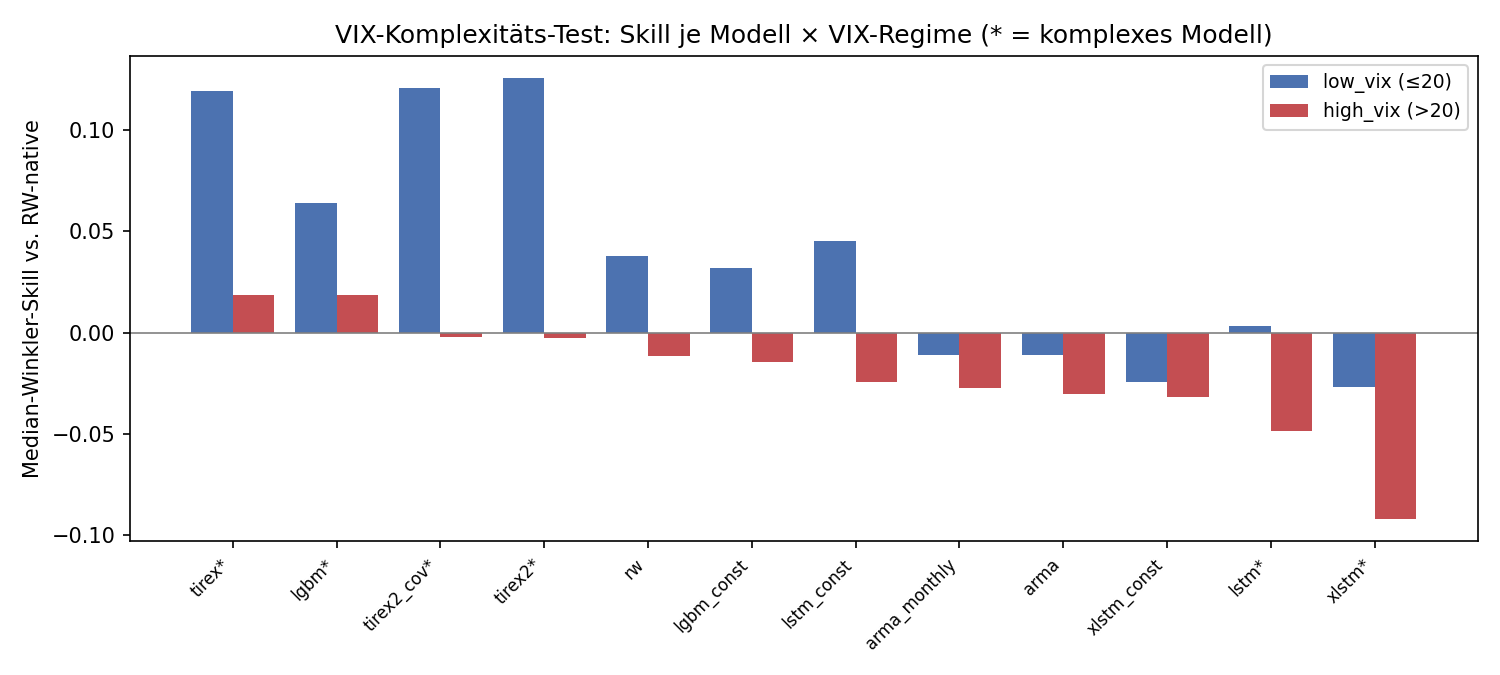
\includegraphics[width=0.8\textwidth]{figures/vix_complexity.png}
%   \caption{% TODO}
%   \label{fig:res_vix}
% \end{figure}
\begin{table}[t]
\centering
\caption{% TODO Caption. The eight largest cross-model contrasts by
         absolute effect size, out of 66. Effect as in
         \cref{tab:res_contrasts}; negative means A is better. None of
         the 66 contrasts is significant after FDR correction.}
\label{tab:res_xm}
\begin{tabular}{llrrrr}
\toprule
A & B & Effect & Share A better & Panel $t$ & median $q$ \\
\midrule
\texttt{tirex2}/ZS/\texttt{cqr\_static}    & \texttt{xlstm\_const}/L/\texttt{spci\_cqr} & $-0.116$ & 0.8 & $-3.55$ & 0.185 \\
\texttt{tirex2\_cov}/ZS/\texttt{native}    & \texttt{xlstm\_const}/L/\texttt{spci\_cqr} & $-0.111$ & 0.9 & $-4.16$ & 0.196 \\
\texttt{tirex}/ZS/\texttt{native}          & \texttt{xlstm\_const}/L/\texttt{spci\_cqr} & $-0.101$ & 1.0 & $-3.26$ & 0.263 \\
\texttt{lgbm}/G/\texttt{decay\_ocp\_cqr}   & \texttt{xlstm\_const}/L/\texttt{spci\_cqr} & $-0.090$ & 0.7 & $-2.92$ & 0.270 \\
\texttt{lstm\_const}/G/\texttt{agaci\_cqr} & \texttt{xlstm\_const}/L/\texttt{spci\_cqr} & $-0.080$ & 0.8 & $-2.43$ & 0.352 \\
\texttt{tirex2\_cov}/ZS/\texttt{native}    & \texttt{arma}/L/\texttt{dtaci\_cqr}        & $-0.075$ & 0.9 & $-3.09$ & 0.217 \\
\texttt{tirex2}/ZS/\texttt{cqr\_static}    & \texttt{lstm}/L/\texttt{pid\_cqr}          & $-0.074$ & 0.9 & $-3.09$ & 0.253 \\
\texttt{tirex2}/ZS/\texttt{cqr\_static}    & \texttt{arma}/L/\texttt{dtaci\_cqr}        & $-0.074$ & 0.9 & $-2.50$ & 0.255 \\
\bottomrule
\end{tabular}
\end{table}

%------------------------------------------------------------------------
\subsection{Economic evaluation}
\label{sec:res:econ}
%------------------------------------------------------------------------
% ERINNERUNG (7.7 + CLAUDE.md): dieser Block ist SEKUNDAER und darf nie
% zum Rangkriterium werden. Der erste Satz muss das sagen.
%
% WAS HIER STEHT:
%  1. Kapital-Proxy: der Median-Kapitalquotient ueber valide Kombis liegt
%     bei 0.669 (Spanne 0.551 bis 0.878). Also: valide, rekalibrierte
%     Intervalle sind im Median rund ein Drittel schmaler als der
%     breiteste valide Benchmark.
%  2. Der eigentlich interessante Befund: die Korrelation zwischen
%     Winkler-Skill und Kapitalquotient betraegt -0.711 (valide Kombis).
%     Hoher Skill geht also systematisch mit niedrigerem Kapitalbedarf
%     einher. -> Das ist die Bruecke von der statistischen zur
%     oekonomischen Metrik und rechtfertigt den Winkler-Score als
%     Rangkriterium nachtraeglich. Guter, zitierfaehiger Satz.
%  3. Der Kontrastbefund, der genauso wichtig ist: die Korrelation
%     zwischen Skill und dem Sharpe der Handelsregel betraegt nur -0.147,
%     also praktisch null und sogar leicht negativ.
%     -> Aussage: bessere Intervalle uebersetzen sich in Kapitaleffizienz,
%        aber NICHT in Handelsgewinne. Genau so schreiben. Das ist ein
%        ehrlicher Befund und schuetzt dich davor, dass jemand die
%        Arbeit als Trading-Paper missversteht.
%  4. Sharpe-Verteilung: Median 0.159, Spanne -0.607 bis 0.621, 68% der
%     validen Kombis haben positiven Sharpe. Der Active Share ist winzig
%     (die Regel handelt nur, wenn der Vormonatsspread ausserhalb des
%     Intervalls lag -- bei ~80% Coverage sind das per Konstruktion
%     wenige Monate). Beispielwerte: 0.003 bis 0.053.
%     -> Ein Satz: bei so wenigen aktiven Monaten ist der Sharpe
%        extrem verrauscht; die Zahl taugt nur zum Methodenvergleich,
%        nicht als Renditeaussage. Transaktionskosten sind ignoriert.
%  5. Die Top-Sharpe-Pakete sind NICHT die Top-Skill-Pakete
%     (lstm/L/pid_cqr 0.621 Sharpe bei nur 0.062 Skill; xlstm/GI/agaci
%     0.446 Sharpe bei NEGATIVEM Skill -0.111). Das ist die konkrete
%     Illustration von Punkt 3 -- unbedingt als Beispiel bringen.
%
% ZAHLEN (verifiziert, econ_results.csv gejoint mit validity_flag=True,
%   485 valide Kombis):
%   median_sharpe    : Median 0.159 | Min -0.607 | Max 0.621 | >0: 68%
%   median_cap_ratio : Median 0.669 | Min 0.551 | Max 0.878
%   corr(median_skill, median_sharpe)    = -0.147
%   corr(median_skill, median_cap_ratio) = -0.711
%   Top-Sharpe (valide): lstm/L/42/pid_cqr 0.621 (Skill 0.062)
%     | lstm_const/G/42/spci 0.609 (Skill 0.060)
%     | lstm_const/GF/43/sfogd 0.484 (Skill 0.016)
%     | lstm/L/42/dtaci 0.482 (Skill 0.057)
%     | xlstm/GI/44/agaci 0.446 (Skill -0.111)
%
% ZITATE: bcbs2019mar (Basel-Kontext, Proxy-Charakter betonen).
%
% [arXiv-Kuerzung]: 3 Saetze -- Kapitalquotient-Median, die beiden
%   Korrelationen, der "kein Trading-Signal"-Satz. Bei hartem Limit:
%   ganzes Unterkapitel in eine Fussnote.


%------------------------------------------------------------------------
\subsection{Robustness}
\label{sec:res:robustness}
%------------------------------------------------------------------------
% WAS HIER STEHT (vier Checks aus 7.8, je 2-3 Saetze):
%  1. KALIBRIERUNGSPOOL. Primaerfall rolling(36) gegen expanding,
%     rolling(24), rolling(48). Auf den 3180 gemeinsamen Zellen betraegt
%     die mittlere absolute Coverage-Differenz zu expanding 0.040
%     (Maximum 0.189), zu rolling24 0.021 (max 0.102), zu rolling48
%     0.016 (max 0.087).
%     -> Ehrlicher Satz: die Pool-Wahl ist NICHT vernachlaessigbar; im
%        Extremfall verschiebt sie die Coverage um fast 19 Prozentpunkte.
%        Die mittlere Coverage steigt mit laengerem Pool
%        (rolling24 0.813 < rolling48 0.820 < rolling 0.834
%        < expanding 0.843), was zur Ueberdeckungsdiagnose aus 8.1 passt:
%        laengere Pools erben alte, breitere Quantile.
%     -> Story-Report F8 nennt lstm/GI/cqr_rolling mit 8.9pp Differenz
%        rolling vs expanding als Extremfall.
%  2. EX-IRLAND. Spearman-Rangkorrelation der Rankings mit und ohne
%     Irland: rho = 0.939 ueber die 485 validen Kombis. Die Rangfolge
%     ist also stabil. ABER das Niveau nicht: der mittlere Skill faellt
%     um -0.021, und beim Spitzenreiter tirex2/ZS/cqr_static von 0.146
%     auf 0.103 (-0.043).
%     -> Zwei Saetze: (i) die Ordnung ist robust, (ii) rund ein Drittel
%        des absoluten Vorsprungs des Siegers stammt aus Irland allein.
%        Da IE mit Skill 0.231 das mit Abstand "leichteste" Land ist und
%        wegen der MNE-/Leprechaun-Verzerrung ohnehin unter Vorbehalt
%        steht, gehoert das prominent berichtet, nicht in eine Fussnote.
%     -> Am staerksten leidet lgbm/L: aci von 0.067 auf -0.027,
%        dtaci von 0.075 auf -0.009, agaci von 0.085 auf 0.009. Also
%        LightGBM im lokalen Regime lebt fast vollstaendig von Irland.
%  3. SEEDS. Nur NN-Modelle (588 Kombinationen ueber xlstm/lstm und ihre
%     const-Zwillinge). Die Seed-Spannweite des Skills betraegt im Median
%     0.043, im Mittel 0.051, maximal 0.315.
%     -> Die entscheidende Zahl: in 52% der NN-Kombinationen ist die
%        Seed-Spannweite GROESSER als der Betrag des Skills selbst.
%        Das heisst, fuer die Haelfte der NN-Ergebnisse ist die
%        Initialisierung ein groesserer Effekt als das Ergebnis.
%        Konsequenz nach der Seed-Disziplin aus 7.8: fuer diese Faelle
%        werden KEINE Rangaussagen getroffen. Diesen Satz explizit
%        schreiben -- er entwertet die schwachen xlstm-Zahlen nicht,
%        er ordnet sie richtig ein.
%     -> Konkreter Beleg aus dem Story-Report (F9): lstm/G/dtaci_cqr
%        mit Seed-Spanne 0.043 ueber dem Effekt.
%     -> Auch relevant fuer 8.3: xlstm/L/native (0.094) hat seed_span
%        0.102 -- die Spanne ist groesser als der Skill. Das beste
%        xlstm-Paket ist also seed-fragil. UNBEDINGT dazuschreiben.
%  4. BURN-IN (F11). Coverage in den ersten 36 Testmonaten gegen den Rest:
%     im Mittel ueber alle Methoden -0.011, also leichte UNTERdeckung
%     am Anfang. Der groesste Effekt liegt bei native (-0.066), gefolgt
%     von decay_ocp (-0.041), saocp (-0.037), cqr_static (-0.034).
%     Die adaptiven Online-Verfahren zeigen praktisch keinen Burn-in-
%     Effekt oder sogar das umgekehrte Vorzeichen (aci +0.015,
%     spci +0.012, dtaci +0.009).
%     -> Interpretation: der Effekt trifft genau die Methoden, die einen
%        gefuellten Kalibrierungspool brauchen, und nicht die, die online
%        nachregeln. Das ist konsistent und selbstlimitierend (mit
%        wachsendem Pool verschwindet er). Ehrlich, aber ohne Dramatik
%        berichten.
%     -> Ein Satz zur Doppelrolle: das HPO-Validierungsfenster dient
%        gleichzeitig als CP-Initialisierung. Das ist die eigentliche
%        Sorge hinter F11; die Messung zeigt, dass sie sich in einer
%        Anfangs-UNTERdeckung aeussert, nicht in kuenstlichem Optimismus.
%  5. Ein letzter Satz zur Laender-Konsistenz (F7): die mittlere paarweise
%     Kendall-Rangkorrelation der Kombinations-Rankings zwischen den
%     Laendern betraegt tau = 0.35. Die Rangfolge ist also nur schwach
%     laenderuebergreifend stabil -- ein weiteres Argument fuer die
%     zurueckhaltende Formulierung aus 8.8.
%
% ZAHLEN (verifiziert):
%   cells.csv, mittlere Coverage je pool_mode:
%     rolling24 0.8127 | rolling48 0.8204 | rolling 0.8341 | expanding 0.8432
%     Median-Skill: rolling24 +0.0003 | rolling48 +0.0142
%       | rolling -0.0126 | expanding -0.0111
%     paarweise |Differenz| auf 3180 gemeinsamen Zellen:
%       vs expanding  mean 0.0397  max 0.1890
%       vs rolling24  mean 0.0208  max 0.1024
%       vs rolling48  mean 0.0156  max 0.0866
%   robustness_ex_ie.csv (485 valide): mean d_skill -0.0210,
%     median -0.0176, Spearman rho(mit vs ohne IE) = 0.9392
%     Top-5 mit/ohne IE: tirex2/cqr_static 0.146->0.103 (-0.043)
%       | tirex2/decay_ocp 0.144->0.100 | tirex2/native 0.142->0.098
%       | tirex2_cov/native 0.141->0.097 | tirex2_cov/cqr_static
%       0.140->0.098
%     groesste Verschlechterung: lgbm/L/aci -0.094 | lgbm/L/dtaci -0.084
%       | lgbm/L/agaci -0.077 | arma_monthly/L/cqr_rolling -0.070
%   ranking_all.csv, seed_span ueber 588 NN-Kombis:
%     Median 0.0431 | Mittel 0.0514 | Max 0.3146
%     Anteil mit seed_span > |median_skill|: 0.52
%   cells.csv, cov_first36 minus cov_rest je Methode:
%     native -0.0664 | decay_ocp -0.0405 | saocp -0.0371 | cqr_static
%     -0.0336 | pid_tan -0.0100 | mondrian -0.0038 | agaci -0.0034
%     | pid_local -0.0025 | sfogd +0.0011 | pid +0.0039 | cqr_rolling
%     +0.0065 | dtaci +0.0090 | spci +0.0121 | aci +0.0146
%     Gesamtmittel: -0.0107
%   story_report.md F7: mittlere paarweise Kendall-tau zwischen
%     Laendern = 0.35
%
% ZITATE: keine neuen Pflichtzitate. Fuer die IE-/Leprechaun-Verzerrung
%   brauchst du EINE Quelle (CSO Irland "Modified GNI (GNI*)") -- steht
%   noch aus, siehe offener Punkt am Ende von evaluation.tex.
%
% [arXiv-Kuerzung]: 1 Absatz mit vier Stichpunkten inline. Die
%   Seed-Fragilitaet und der ex-IE-Niveaueffekt MUESSEN drin bleiben.


%------------------------------------------------------------------------
\subsection{Summary of findings}
\label{sec:res:summary}
%------------------------------------------------------------------------
% WAS HIER STEHT: 6-8 nummerierte Saetze, je einer pro Kernbefund, jeweils
% mit der tragenden Zahl. Das ist die Vorlage fuer Abstract und Conclusion
% -- schreib es so, dass du es dort fast woertlich wiederverwenden kannst.
%
% VORSCHLAG DER REIHENFOLGE (inhaltlich, du formulierst):
%  (1) Punktprognose: kein Modell schlaegt den Random Walk; das beste
%      MAE-Verhaeltnis ist 0.997 (tirex2), alle trainierten Modelle
%      liegen darueber.
%  (2) Kalibrierung: native Modellquantile sind systematisch ueberdeckend
%      (0.872 statt 0.80) und passieren das Gate nur in 13% der Faelle;
%      adaptive CP-Verfahren erreichen 96-100%.
%  (3) Intervallguete: das beste valide Paket ist ein Zero-Shot-
%      Foundation-Model (tirex2/ZS, Skill 0.14-0.15) vor dem besten
%      klassischen Ansatz (rw/L/aci_cqr, 0.085).
%  (4) Aber: kein einziger der 66 Cross-Model-Kontraste ist FDR-
%      signifikant (min. median-q 0.185), und die MCS schliesst fast
%      nichts aus. Die Rangfolge ist deskriptiv.
%  (5) Kovariaten: der ceteris-paribus-Kontrast ist null
%      (d_norm -0.00006, p 0.45); 17 makrooekonomische Kovariaten
%      liefern dem vortrainierten Modell keine Zusatzinformation.
%  (6) Pooling und Adaptivitaet: globales Pooling hilft den neuronalen
%      Modellen nicht (+0.017), Fine-Tuning schlaegt Laender-Embedding
%      klar (-0.054), und modelleigene adaptive Breiten sind im Median
%      schlechter als konstante (+0.020).
%  (7) xLSTM: die namensgebende Architektur ist die schwaechste Familie
%      (Median-Skill -0.047); das beste valide Paket ist seed-fragil
%      (Skill 0.094 bei Seed-Spanne 0.102).
%  (8) Regime: der Vorsprung der komplexen Modelle verschwindet im
%      Stress (Delta -0.077 von low- zu high-VIX; tirex2 von 0.125
%      auf -0.003).
%
% !! Wenn du (3) schreibst, muss die Entscheidung aus 8.3 Punkt 4
%    (cqr_static vs decay_ocp) hier konsistent durchgezogen sein.
%
% [arXiv-Kuerzung]: bleibt vollstaendig, das ist das Rueckgrat des Papers.


%========================================================================
%  ANSCHLUSS-KAPITEL
%------------------------------------------------------------------------
%  LIMITATIONS -- seit 2026-08-03 ein eigenes Kapitel:
%    sections/limitations.tex, eingebunden in main.tex nach diesem Kapitel.
%    Alle Punkte, die in diesem Results-Kapitel aufgeworfen werden, sind
%    dort in acht Unterkapiteln ausgeschrieben (9.1 Kontamination,
%    9.2 Gate/DQ, 9.3 Inferenz+Power, 9.4 Seeds, 9.5 Stichprobe/Panel,
%    9.6 Designentscheidungen, 9.7 Oekonomie, 9.8 Scope).
%    -> Neue Limitationen NICHT mehr hier sammeln, sondern direkt dort
%       einsortieren. Diese Liste ist bewusst geloescht, damit es keine
%       zweite Wahrheit gibt.
%    -> Aus diesem Kapitel sollten Vorwaertsverweise gesetzt werden:
%       8.1 Gate -> \cref{sec:lim:gate}
%       8.2 Punktprognose -> \cref{sec:lim:scope} (PT-Artefakt, DM-Test)
%       8.3 Ranking -> \cref{sec:lim:contamination} und \cref{sec:lim:seeds}
%       8.8 Cross-Model/MCS -> \cref{sec:lim:inference}
%       8.11 Robustheit -> \cref{sec:lim:sample} (ex-IE) und
%                          \cref{sec:lim:design} (Pool-Fenster)
%
%  Discussion -- noch nicht angelegt. Abgrenzung zu den Limitations:
%    dort steht, was die Befunde BEDEUTEN (warum Zero-Shot gewinnt, warum
%    xLSTM verliert, was das fuer die Praxis heisst), hier steht, wo sie
%    an ihre Grenzen stossen. Nicht vermischen.
%  Conclusion -- 1-2 Seiten, gestuetzt auf 8.12.
%========================================================================

% \input{sections/discussion}
% \input{sections/conclusion}

% ... letztes reguläres Kapitel endet hier ...

\appendix

\begin{table}[htbp]
  \centering\small
  \caption{Selected (frozen) configurations per model and regime, chosen once on
  the burn-in and held fixed for all refit blocks. RW and ARMA are deterministic;
  the deep models additionally use seeds 42/43/44.}
  \label{tab:app_frozen}
  \begin{tabular}{@{}lll@{}}
    \toprule
    \textbf{Model} & \textbf{Regime} & \textbf{Selected configuration} \\
    \midrule
    Random Walk & L  & ARMA(0,0), trend $=$ none (no free parameters) \\
    \addlinespace
    ARMA        & L  & per country: AT/BE/ES/FI/IE $(2,2)$; FR $(0,0)$; \\
                &    & \quad GR $(3,2)$; IT $(3,0)$; NL $(2,3)$; PT $(3,3)$ \\
    \addlinespace
    LightGBM    & L  & lag $\{1\}$, no rolling means, lr $0.15$, num\_leaves $7$, \\
                &    & \quad max\_depth $-1$, min\_data\_in\_leaf $5$, feature\_fraction $0.78$, \\
                &    & \quad bagging\_fraction $0.51$, $\lambda_1\,0.019$, $\lambda_2\,0.34$ \\
    \addlinespace
    LightGBM    & G  & lag $\{1\}$, rolling means, lr $0.083$, num\_leaves $15$, \\
                &    & \quad max\_depth $3$, min\_data\_in\_leaf $40$, feature\_fraction $0.53$, \\
                &    & \quad bagging\_fraction $0.74$, $\lambda_1\,0.013$, $\lambda_2\,8.1\times10^{-6}$ \\
    \addlinespace
    LSTM        & L  & lookback $3$, hidden $64$, $29$ epochs \\
    LSTM        & G  & lookback $3$, hidden $32$, $10$ epochs \\
    LSTM        & GF & init from G, lr $\times 0.1$, $20$ fine-tune epochs \\
    \addlinespace
    xLSTM       & L  & lookback $3$, mLSTM, $1$ block, dim $32$, $5$ epochs \\
    xLSTM       & G  & lookback $24$, mLSTM, $3$ blocks, dim $64$, $1$ epoch \\
    xLSTM       & GF & init from G, lr $\times 0.1$, $5$ fine-tune epochs \\
    \addlinespace
    TiRex-2     & ZS & zero-shot, no tuned parameters (variants \texttt{tirex2}, \texttt{tirex2\_cov}) \\
    \bottomrule
  \end{tabular}
\end{table}

The search protocol is shared across all tuned models (\cref{tab:app_protocol});
the model-specific search spaces are given in \cref{tab:app_nn_space}
(sequence models) and \cref{tab:app_lgbm_space} (LightGBM). Every configuration
is selected once on the burn-in and frozen thereafter (\cref{tab:app_frozen}).

\begin{table}[htbp]
  \centering\small
  \caption{Shared hyperparameter-search protocol.}
  \label{tab:app_protocol}
  \begin{tabular}{@{}ll@{}}
    \toprule
    \textbf{Setting} & \textbf{Value} \\
    \midrule
    Search algorithm            & Optuna, TPE sampler (seed 42) \\
    Trials per study            & 100 (20 random start-up trials) \\
    Pruner                      & MedianPruner (20 start-up trials, 3 warm-up steps) \\
    Studies                     & one per regime (L, G) \\
    Selection window            & train $\le$ month 114, validate months 115--150 \\
    Selection metric            & mean standardized-$\Delta$ pinball loss, averaged over countries \\
    Epoch ceiling / early stop (NN) & 100 epochs / patience 15, restore-best \\
    Boosting-round early stop (LightGBM) & 50 rounds \\
    GF fine-tuning              & learning rate $\times\,0.1$, epochs from $\{5,10,20,40\}$ \\
    Country embedding dim (NN, regime G) & 8 \\
    Seeds                       & 42, 43, 44 \\
    Information-horizon cap     & 24 months \\
    \bottomrule
  \end{tabular}
\end{table}

\begin{table}[htbp]
  \centering\small
  \caption{Sequence-model hyperparameter search spaces. Shared rows are
  identical by design; ``---'' marks a parameter that does not exist for that
  architecture.}
  \label{tab:app_nn_space}
  \resizebox{\textwidth}{!}{%
  \begin{tabular}{@{}lll@{}}
    \toprule
    \textbf{Hyperparameter} & \textbf{LSTM} & \textbf{xLSTM} \\
    \midrule
    lookback\_window       & $\{3,6,12,18,24\}$ & $\{3,6,12,18,24\}$ \\
    learning\_rate         & $[10^{-4},10^{-2}]$ log & $[10^{-4},10^{-2}]$ log \\
    weight\_decay          & $[10^{-6},10^{-2}]$ log & $[10^{-6},10^{-2}]$ log \\
    batch\_size            & $\{16,32,64\}$ & $\{16,32,64\}$ \\
    gradient\_clip         & $[0.5,5.0]$ & $[0.5,5.0]$ \\
    optimizer              & \{adam, adamw\} & \{adam, adamw\} \\
    scheduler              & \{none, cosine\} & \{none, cosine\} \\
    dropout                & $[0.0,0.4]$ & $[0.0,0.4]$ \\
    hidden / embedding dim & $\{32,64,128\}$ & $\{32,64,128\}$ \\
    depth                  & num\_layers $\{1,2,3\}$ & num\_blocks $\{1,2,3,4\}$ \\
    arch                   & --- & \{mlstm\_only, mixed\} \\
    conv1d\_kernel\_size   & --- & $\{3,5,7\}$ ($\le$ lookback) \\
    num\_heads             & --- & $\{2,4\}$ \\
    qkv\_proj\_blocksize   & --- & $\{2,4\}$ \\
    proj\_factor (mLSTM)   & --- & $[1.0,2.5]$ \\
    proj\_factor (sLSTM)   & --- & $[1.0,1.5]$ \\
    activation             & --- & \{gelu, relu\} \\
    bias\_init             & --- & \{powerlaw\_blockdependent, small\_init, standard\} \\
    \bottomrule
  \end{tabular}%
  }
\end{table}

\begin{table}[htbp]
  \centering\small
  \caption{LightGBM hyperparameter search space. A booster is fitted per
  quantile. \texttt{lag\_set} selects one of the six nested lag sets
  $\{1\},\{1,2\},\{1,2,3\},\{1,2,3,6\},\{1,2,3,6,12\},\{1,2,3,6,12,24\}$;
  in regime G the country enters as a native categorical feature.}
  \label{tab:app_lgbm_space}
  \begin{tabular}{@{}ll@{}}
    \toprule
    \textbf{Hyperparameter} & \textbf{Range} \\
    \midrule
    lag\_set          & one of six nested sets (see caption) \\
    rolling\_means    & \{true, false\} (means over $\{3,6,12\}$ months) \\
    learning\_rate    & $[0.01, 0.3]$ log \\
    num\_leaves       & $\{7, 15, 31\}$ \\
    max\_depth        & $\{-1, 3, 5, 7\}$ \\
    min\_data\_in\_leaf & $\{5, 10, 20, 40\}$ \\
    feature\_fraction & $[0.5, 1.0]$ \\
    bagging\_fraction & $[0.5, 1.0]$ \\
    lambda\_l1        & $[10^{-8}, 10]$ log \\
    lambda\_l2        & $[10^{-8}, 10]$ log \\
    \bottomrule
  \end{tabular}
\end{table}

% ============================================================
% APPENDIX — FROZEN HYPERPARAMETERS
% ============================================================

\begin{table}[htbp]
  \centering\small
  \caption{Frozen neural-network hyperparameters, one column per model and
  regime. Values marked ``---'' do not apply to that architecture. ``Depth''
  is the number of xLSTM blocks / LSTM layers; ``width'' is the xLSTM embedding
  dimension / LSTM hidden size. Frozen epochs are the production epoch counts
  taken from the winning trial. GF fine-tuning uses learning rate $\times\,0.1$.}
  \label{tab:app_frozen_nn}
  \begin{tabular}{@{}lcccc@{}}
    \toprule
    & \textbf{xLSTM (L)} & \textbf{xLSTM (G)} & \textbf{LSTM (L)} & \textbf{LSTM (G)} \\
    \midrule
    Lookback window $W$        & 3     & 24    & 3     & 3 \\
    Architecture               & mLSTM-only & mLSTM-only & --- & --- \\
    Depth (blocks / layers)    & 1     & 3     & 1     & 2 \\
    Width (embed. / hidden)    & 32    & 64    & 64    & 32 \\
    conv1d kernel size         & 3     & 7     & ---   & --- \\
    Heads                      & 2     & 2     & ---   & --- \\
    qkv projection blocksize   & 4     & 4     & ---   & --- \\
    Projection factor (mLSTM)  & 2.13  & 2.36  & ---   & --- \\
    Bias init                  & powerlaw & powerlaw & --- & --- \\
    Activation (block FFN)     & gelu  & gelu  & ---   & --- \\
    Dropout                    & 0.037 & 0.265 & 0.343 & 0.030 \\
    Learning rate              & $3.46\times10^{-3}$ & $2.95\times10^{-4}$ & $2.01\times10^{-4}$ & $1.98\times10^{-3}$ \\
    Weight decay               & $1.16\times10^{-3}$ & $6.23\times10^{-5}$ & $1.87\times10^{-4}$ & $1.54\times10^{-4}$ \\
    Batch size                 & 64    & 16    & 16    & 32 \\
    Gradient clip              & 3.23  & 2.03  & 4.36  & 4.82 \\
    Optimizer                  & Adam  & Adam  & AdamW & Adam \\
    LR scheduler               & none  & none  & none  & cosine \\
    Frozen epochs (production) & 5     & 1     & 29    & 10 \\
    GF fine-tune epochs        & ---   & 5     & ---   & 20 \\
    \bottomrule
  \end{tabular}
\end{table}

\begin{table}[htbp]
  \centering\small
  \caption{Frozen LightGBM hyperparameters. One booster is fitted per quantile.
  The lag set is the tabular replacement for a lookback window; rolling means are
  taken over $\{3,6,12\}$ months. \texttt{max\_depth}${}=-1$ means no depth limit
  (leaf-wise growth is bounded by \texttt{num\_leaves}).}
  \label{tab:app_frozen_lgbm}
  \begin{tabular}{@{}lcc@{}}
    \toprule
    \textbf{Hyperparameter} & \textbf{L} & \textbf{G} \\
    \midrule
    Lag set              & $\{1\}$ & $\{1\}$ \\
    Rolling means        & no    & yes \\
    Learning rate        & 0.153 & 0.083 \\
    \texttt{num\_leaves} & 7     & 15 \\
    \texttt{max\_depth}  & $-1$  & 3 \\
    \texttt{min\_data\_in\_leaf} & 5 & 40 \\
    Feature fraction     & 0.776 & 0.532 \\
    Bagging fraction     & 0.514 & 0.735 \\
    $\lambda_{L1}$       & 0.0185 & 0.0125 \\
    $\lambda_{L2}$       & 0.341 & $8.11\times10^{-6}$ \\
    \bottomrule
  \end{tabular}
\end{table}

\begin{table}[htbp]
  \centering\small
  \caption{Frozen ARIMA orders per country, selected by AIC over
  $(p,q)\in\{0,\dots,3\}^2$ on the differenced target (regime L only). France
  collapses to $(0,0)$, i.e.\ a random walk on the differenced series. The Random
  Walk itself has no tunable hyperparameters.}
  \label{tab:app_frozen_arma}
  \begin{tabular}{@{}lcccccccccc@{}}
    \toprule
    & AT & BE & ES & FI & FR & GR & IE & IT & NL & PT \\
    \midrule
    $p$ & 2 & 2 & 2 & 2 & 0 & 3 & 2 & 3 & 2 & 3 \\
    $q$ & 2 & 2 & 2 & 2 & 0 & 2 & 2 & 0 & 3 & 3 \\
    \bottomrule
  \end{tabular}
\end{table}

\section{Result breakdowns}
\label{app:breakdowns}

\begin{table}[t]
\centering
\caption{% TODO Caption. Per-country breakdown. Gate rate is the share of
         admissible cells; median skill is over admissible combinations;
         tail asymmetry is the share of lower violations; base rate is
         $\max(p_{\uparrow},1-p_{\uparrow})$ of the realised direction.}
\label{tab:app_country}
\begin{tabular}{lccccc}
\toprule
Country & Gate rate & Median skill & Tail asym. & Base rate & Mean Kendall $\tau$ \\
\midrule
GR & 0.519 & $ 0.120$ & 0.594 & 0.591 & 0.345 \\
PT & 0.616 & $ 0.191$ & 0.572 & 0.646 & 0.392 \\
IE & 0.623 & $ 0.231$ & 0.642 & 0.575 & 0.341 \\
ES & 0.660 & $ 0.095$ & 0.567 & 0.583 & 0.408 \\
BE & 0.718 & $ 0.051$ & 0.502 & 0.559 & 0.418 \\
AT & 0.747 & $-0.015$ & 0.551 & 0.583 & 0.373 \\
NL & 0.771 & $-0.002$ & 0.552 & 0.591 & 0.341 \\
IT & 0.810 & $-0.070$ & 0.444 & 0.575 & 0.225 \\
FI & 0.844 & $-0.052$ & 0.431 & 0.598 & 0.280 \\
FR & 0.864 & $-0.047$ & 0.504 & 0.520 & 0.335 \\
\bottomrule
\end{tabular}
\end{table}

\begin{table}[t]
\centering
\caption{% TODO Caption. Tail asymmetry (share of lower violations among
         all violations; 0.5 is symmetric) over admissible combinations,
         by model family and by recalibration method.}
\label{tab:app_tail}
\begin{tabular}{lc@{\hskip 2cm}lc}
\toprule
Model & Tail asym. & Method & Tail asym. \\
\midrule
\texttt{xlstm}        & 0.483 & \texttt{cqr\_static}     & 0.471 \\
\texttt{tirex2}       & 0.510 & \texttt{mondrian\_cqr}   & 0.522 \\
\texttt{tirex2\_cov}  & 0.532 & \texttt{decay\_ocp\_cqr} & 0.522 \\
\texttt{lstm}         & 0.533 & \texttt{sfogd\_cqr}      & 0.528 \\
\texttt{lstm\_const}  & 0.540 & \texttt{dtaci\_cqr}      & 0.529 \\
\texttt{xlstm\_const} & 0.540 & \texttt{pid\_cqr}        & 0.530 \\
\texttt{tirex}        & 0.555 & \texttt{pid\_local\_cqr} & 0.533 \\
\texttt{lgbm\_const}  & 0.577 & \texttt{cqr\_rolling}    & 0.536 \\
\texttt{rw}           & 0.604 & \texttt{saocp\_cqr}      & 0.540 \\
\texttt{arma}         & 0.608 & \texttt{aci\_cqr}        & 0.540 \\
\texttt{lgbm}         & 0.611 & \texttt{agaci\_cqr}      & 0.543 \\
\texttt{arma\_monthly}& 0.618 & \texttt{spci\_cqr}       & 0.553 \\
                      &       & \texttt{native}          & 0.556 \\
                      &       & \texttt{pid\_tan\_cqr}   & 0.562 \\
\bottomrule
\end{tabular}
\end{table}

\begin{table}[t]
\centering
\caption{% TODO Caption. Mean coverage (\%) by calibration-pool window.
         Target is 80\%. Online trackers do not read the pool, so the
         window variants do not apply to them.}
\label{tab:app_pool}
\begin{tabular}{lcccc}
\toprule
Method & rolling 36 & expanding & rolling 24 & rolling 48 \\
\midrule
\texttt{aci\_cqr}        & 81.5 & 84.2 & 81.7 & 81.8 \\
\texttt{agaci\_cqr}      & 81.1 & 82.3 & 81.5 & 81.5 \\
\texttt{cqr\_rolling}    & 82.3 & 85.3 & 80.7 & 83.6 \\
\texttt{cqr\_static}     & 85.9 & 85.9 & --   & --   \\
\texttt{decay\_ocp\_cqr} & 87.3 & 87.3 & --   & --   \\
\texttt{dtaci\_cqr}      & 82.2 & 84.8 & 81.8 & 82.7 \\
\texttt{mondrian\_cqr}   & 86.0 & 86.6 & 87.8 & 85.1 \\
\texttt{native}          & 87.2 & 87.2 & --   & --   \\
\texttt{pid\_cqr}        & 81.3 & 81.3 & --   & --   \\
\texttt{pid\_local\_cqr} & 81.4 & 81.4 & --   & --   \\
\texttt{pid\_tan\_cqr}   & 82.4 & 82.4 & --   & --   \\
\texttt{saocp\_cqr}      & 91.7 & 91.7 & --   & --   \\
\texttt{sfogd\_cqr}      & 80.6 & 80.6 & --   & --   \\
\texttt{spci\_cqr}       & 76.9 & 79.5 & 74.2 & 77.7 \\
\midrule
All cells                & 83.4 & 84.3 & 81.3 & 82.0 \\
Median skill             & $-0.013$ & $-0.011$ & $0.000$ & $0.014$ \\
\bottomrule
\end{tabular}
\end{table}

\begin{table}[t]
\centering
\caption{% TODO Caption. Left: seed dispersion of the neural families.
         Right: median skill of the best admissible package per family,
         recomputed with Ireland excluded from the aggregation.}
\label{tab:app_fragility}
\begin{tabular}{lccc@{\hskip 1.2cm}lcc}
\toprule
NN family & Med.\ span & Max span & span $>|$skill$|$ & Best package & Skill & ex-IE \\
\midrule
\texttt{lstm\_const}  & 0.015 & 0.062 & 0.238 & \texttt{tirex2}       & 0.146 & 0.103 \\
\texttt{xlstm\_const} & 0.045 & 0.126 & 0.587 & \texttt{tirex2\_cov}  & 0.141 & 0.097 \\
\texttt{lstm}         & 0.046 & 0.315 & 0.685 & \texttt{lgbm}         & 0.139 & 0.120 \\
\texttt{xlstm}        & 0.051 & 0.142 & 0.506 & \texttt{tirex}        & 0.133 & 0.094 \\
                      &       &       &       & \texttt{lstm\_const}  & 0.111 & 0.087 \\
                      &       &       &       & \texttt{lgbm\_const}  & 0.099 & 0.071 \\
                      &       &       &       & \texttt{xlstm}        & 0.094 & 0.053 \\
                      &       &       &       & \texttt{rw}           & 0.085 & 0.022 \\
                      &       &       &       & \texttt{xlstm\_const} & 0.072 & 0.068 \\
                      &       &       &       & \texttt{lstm}         & 0.062 & 0.031 \\
                      &       &       &       & \texttt{arma\_monthly}& 0.061 & $-0.005$ \\
                      &       &       &       & \texttt{arma}         & 0.058 & $-0.002$ \\
\bottomrule
\end{tabular}
\end{table}

% optional weitere Anhänge:
\section{Additional descriptive statistics}
\label{app:descriptive}

% ... danach erst:
\printbibliography   % (biblatex)  ODER  \bibliography{...} (bibtex)

\printbibliography
\end{document}
